A detailed description of the SNO+ detector has been implemented in the \texttt{RAT} software package for Monte Carlo (MC) simulations, as mentioned in Chapter 3. However, when the simulations are compared to the real world, there always exist discrepancies. To make precise measurements, calibration sources were implemented in the SNO+ detector during the water phase and the partial-fill phase. During the water phase, the $^{16}$N source (described in Sect.~\ref{sect:n16}, Chapter 3) was used for the primary detector calibration. The $^{16}$N calibration data ($^{16}$N runs) were mainly used for checking the performances of the reconstruction of the event position, direction, and energy. 

In this chapter, the \texttt{MPW fitter} (described in Sect.~\ref{sect:mpw}, Chapter 4) was applied on both the data and simulations of the $^{16}$N runs in the water phase. By comparing the differences between the data and MC, systematics of the position and direction reconstruction were extracted. The event energy was reconstructed by the SNO+ energy fitter for the water phase (described in Sect.~\ref{sect:energyFitter}, Chapter 4), which utilizes the \texttt{MPW fitter} fitted event vertex and direction. Also, based on the \texttt{MPW fitter} reconstructed vertex and direction results, the other parameters, such as the in-time-ratio ($ITR$) and the isotropic parameter ($\beta_{14}$) were calculated. By comparing the $^{16}$N data and the MC simulations, the relevant systematics were also evaluated. These systematic results were used in the solar neutrino analysis in Chapter 6.

\section{\isotope[16]{N} Calibration Scans in the Water Phase}\label{sect:n16_water}
During the water phase, the $^{16}$N source was deployed at different positions inside the AV in June and in November 2017 to perform internal calibration scans. It was also deployed at different positions in the external water region between the AV and the PSUP in March 2018 to perform external scans. For each $^{16}$N run, the source was placed at a fixed position, and the data were taken for about 20 minutes (for the central run-107055, it took 1 hour). The source was inside the AV for the internal scans, moving along x, y, and z-axes (called ``X, Y, Z scans'' in this thesis). It was also was moved diagonally across the AV and was placed at the corners of the inner AV (``corner scans''). For the external scans, the source was placed in the external water region but outside the AV. The source was moved along the z-axis with a fixed $(x,y)$ position close to the AV at (-5861.0,-2524.0)~mm. Fig.~\ref{N16_3Dscan} shows the different positions of the source deployment. In this thesis, 79 internal scan runs were used. Details of the calibration runs are listed in the tables in Appendix.~\ref{appendix:calibration}. %%%%%% and 19 external runs

\begin{figure}[!htb]
	\centering
	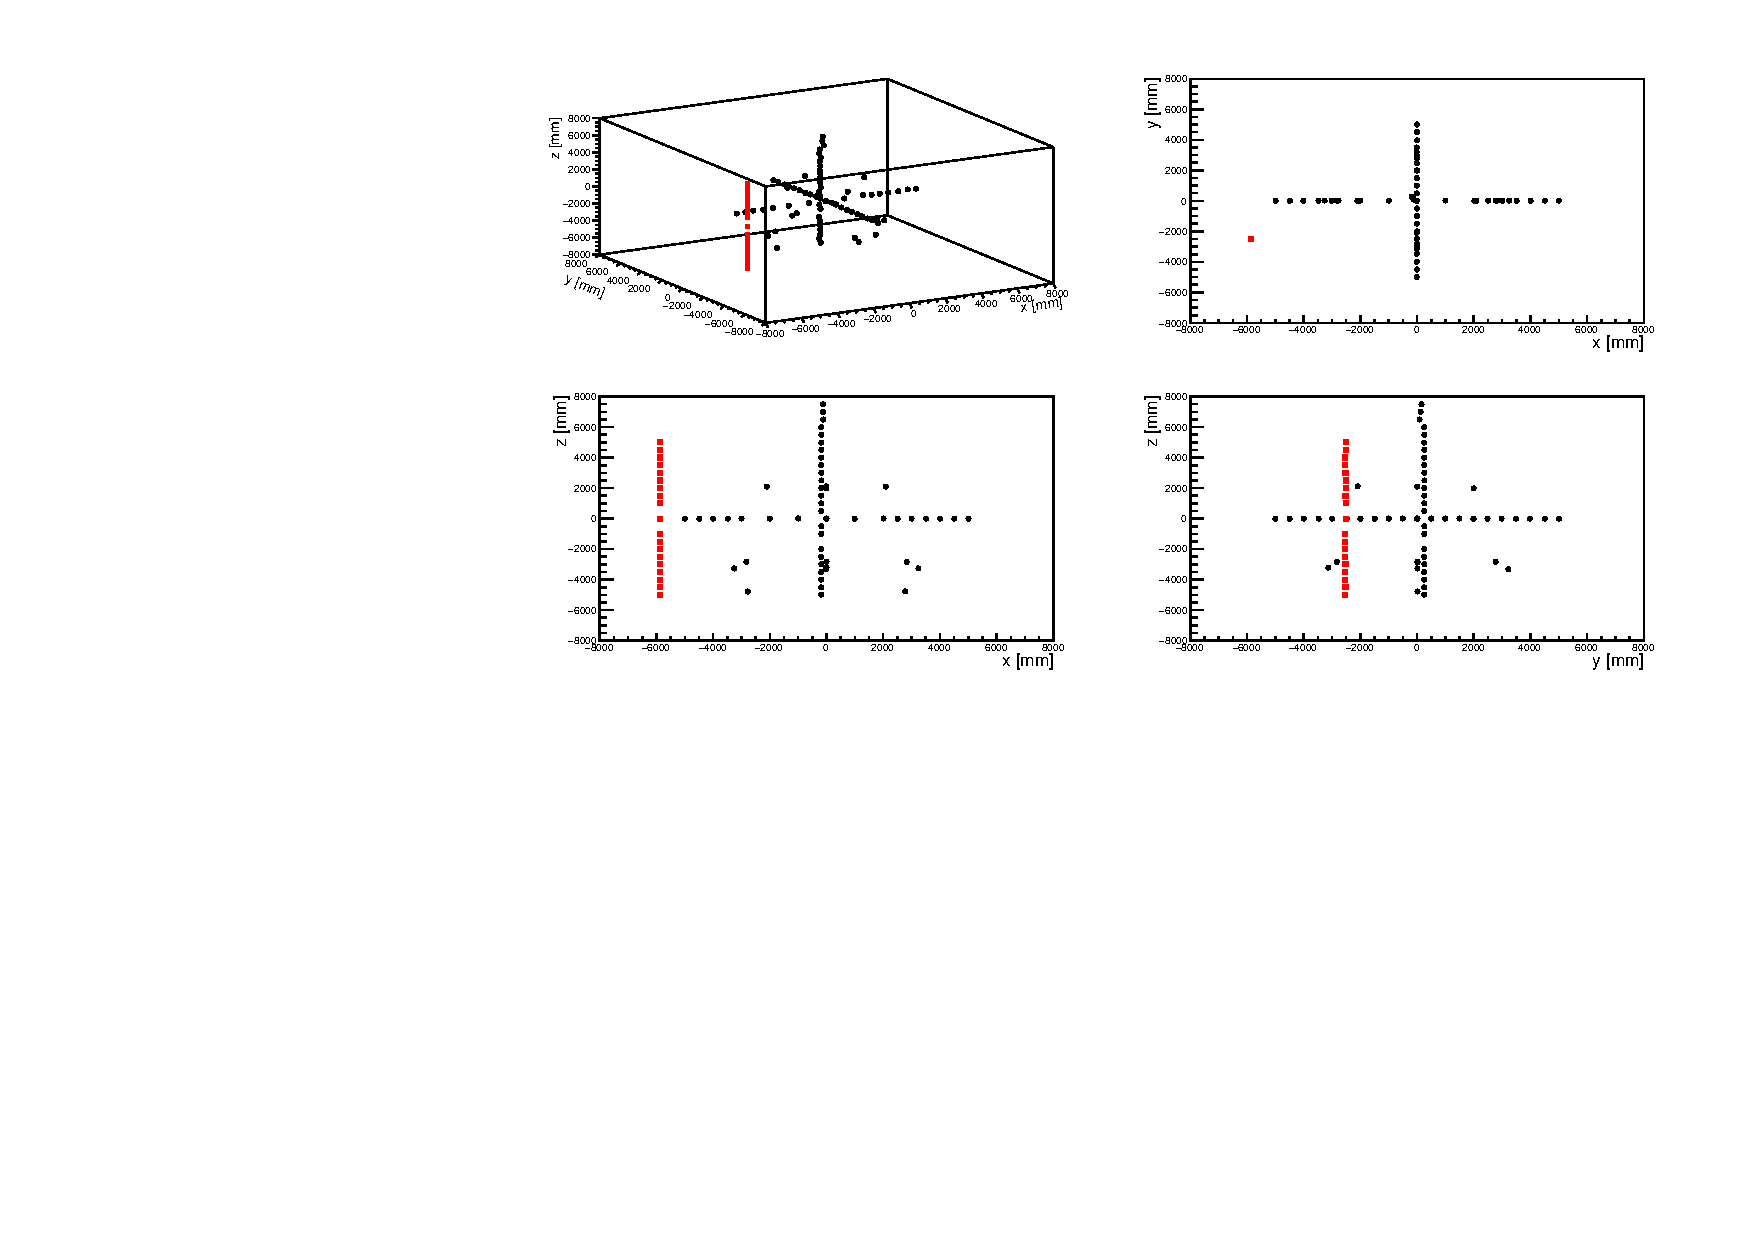
\includegraphics[width=15cm]{N16_3Dscan.pdf}
	\caption[The deployed source positions of the $^{16}$N scan runs.]{The deployed source positions of the $^{16}$N scan runs used by this thesis. The black dots are internal runs while the red squares are external runs.}
	\label{N16_3Dscan}
\end{figure}

The $^{16}$N calibration runs provide ideal tests for the fitter performance. From a comparison of reconstructions for data and MC, we can also extract the resolution and bias of the fitter. Here I worked out the vertex and the direction reconstruction performances for both of the \texttt{RAT water fitter} and the \texttt{MPW fitter}. The vertex shifts as well as the uncertainties were evaluated. 

To tackle with the $^{16}$N run data and simulations, an FECD tag cut ($FECD==9188$) was applied during the data processing, to save the events only when the source trigger fired. A reconstruction threshold on NHits$\geq 6$ was applied to the MC and data. Besides these cuts, high-level cuts based on classifiers were used. 

\section{High Level Cuts for the Water Phase}\label{sect:high_level_cuts}
A set of classifiers were developed by SNO analysis and been optimized for the SNO+ water analysis\cite{highlevel}. These classifiers utilized the reconstructed quantities, so they always require valid reconstructions.

\begin{itemize}
	\item[$\bullet$] In time ratio ($ITR$) classifier
	
	For each event, this classifier loops the triggered PMTs (hits), calculates the $t_{res}$, and then finds the ratio of the number of hits in an optimized prompt time window. In the water phase, the time window was [-2.5,5.0]~ns. If the $ITR$ ratio is too low for an event, it indicates that most of the triggered PMTs are not caused by the prompt lights and thus the event probably does not originate from Cherenkov lights; it can be an instrumental noise, or caused by a large amount of lights reflecting off the detector components (called ``late lights''). 
	
	\item[$\bullet$] $\beta_{14}$ isotropy classifier
	
	This classifier uses Legendre polynomials to return the	first ($\beta_1$) and the fourth ($\beta_4$) spherical harmonics of an event, where:
	\begin{equation}
	\beta_l = \frac{2}{N(N-1)}\sum_{i=1}^{N-1}\sum_{j=i+1}^N P_l(\cos\theta_{ij}),
	\end{equation}
	and $P_l(\cos\theta_{ij})$ are Legendre polynomials. 
	
	A combination of two $\beta_l$ terms was chosen by the SNO collaboration to be: $\beta_{14}=\beta_1+4\beta_4$. This quantity gives a gaussian-like distribution for Cherenkov events\cite{dunmore2004separation}.	In principle, any deviation from zero suggests some polarity or a deviation from a totally isotropic pattern.
	
	\item[$\bullet$] $\theta_{ij}$ isotropy classifier 
	
	This classifier describes the angle subtended at an event vertex by PMT \#i and PMT \#j, which is calculated as:
	\begin{equation}
	\cos\theta_{ij}=\frac{(\vec{X}_{PMT\#i}- \vec{X}_{event})\cdot (\vec{X}_{PMT\#j}- \vec{X}_{event})}{|\vec{X}_{PMT\#i}- \vec{X}_{event}||\vec{X}_{PMT\#j}- \vec{X}_{event}|}.
	\end{equation}
\end{itemize}

\subsection{Effects of the High-level Cuts}
As described above, the classifiers can help to distinguish the signals from Cherenkov events and backgrounds from non-Cherenkov events. To remove the non-Cherenkov backgrounds, cuts of $ITR>0.55$ and $-0.12<\beta_{14}<0.95$ (called ``high-level cuts'') were suggested by the collaboration\cite{waterunidoc}. These cuts are based on the analyses of data cleaning, simulated physics events as well as the SNO experience\cite{waterunidoc,marzec2019measurement,dunmore2004separation}.

The $^{16}$N central run-107055 data and MC were used to check the effects of the high-level cuts. For the MC (data), the cut of $ITR>0.55$ removed 0.69\% (0.79\%) of the total events; $-0.12<\beta_{14}<0.95$ removes 1.11\% (0.93\%) of the total events. Combining the $ITR$ and $\beta_{14}$ cuts, 1.69\% (1.62\%) of the total events were removed.

The poorly reconstructed events with large position biases ($>6000~mm$) were counted.
For the MC case, the position biases were taken as the distance between the reconstructed positions and the true positions generated by the MC: $|\vec{X}_{fit}-\vec{X}_{MC}|$; while for the data case, the biases were between the reconstructed positions and the source manipulation position: $|\vec{X}_{fit}-\vec{X}_{src}|$. The large biased events are 0.13\% of the total events in both the MC and data. The high-level cuts removed 73.12\% (66.82\%) of them for the MC (data).

Fig.~\ref{n16_highLevelCut} shows the relations between the position biases and the $ITR$, $\beta_{14}$ respectively, for the data and MC.
\begin{figure}
	\centering
	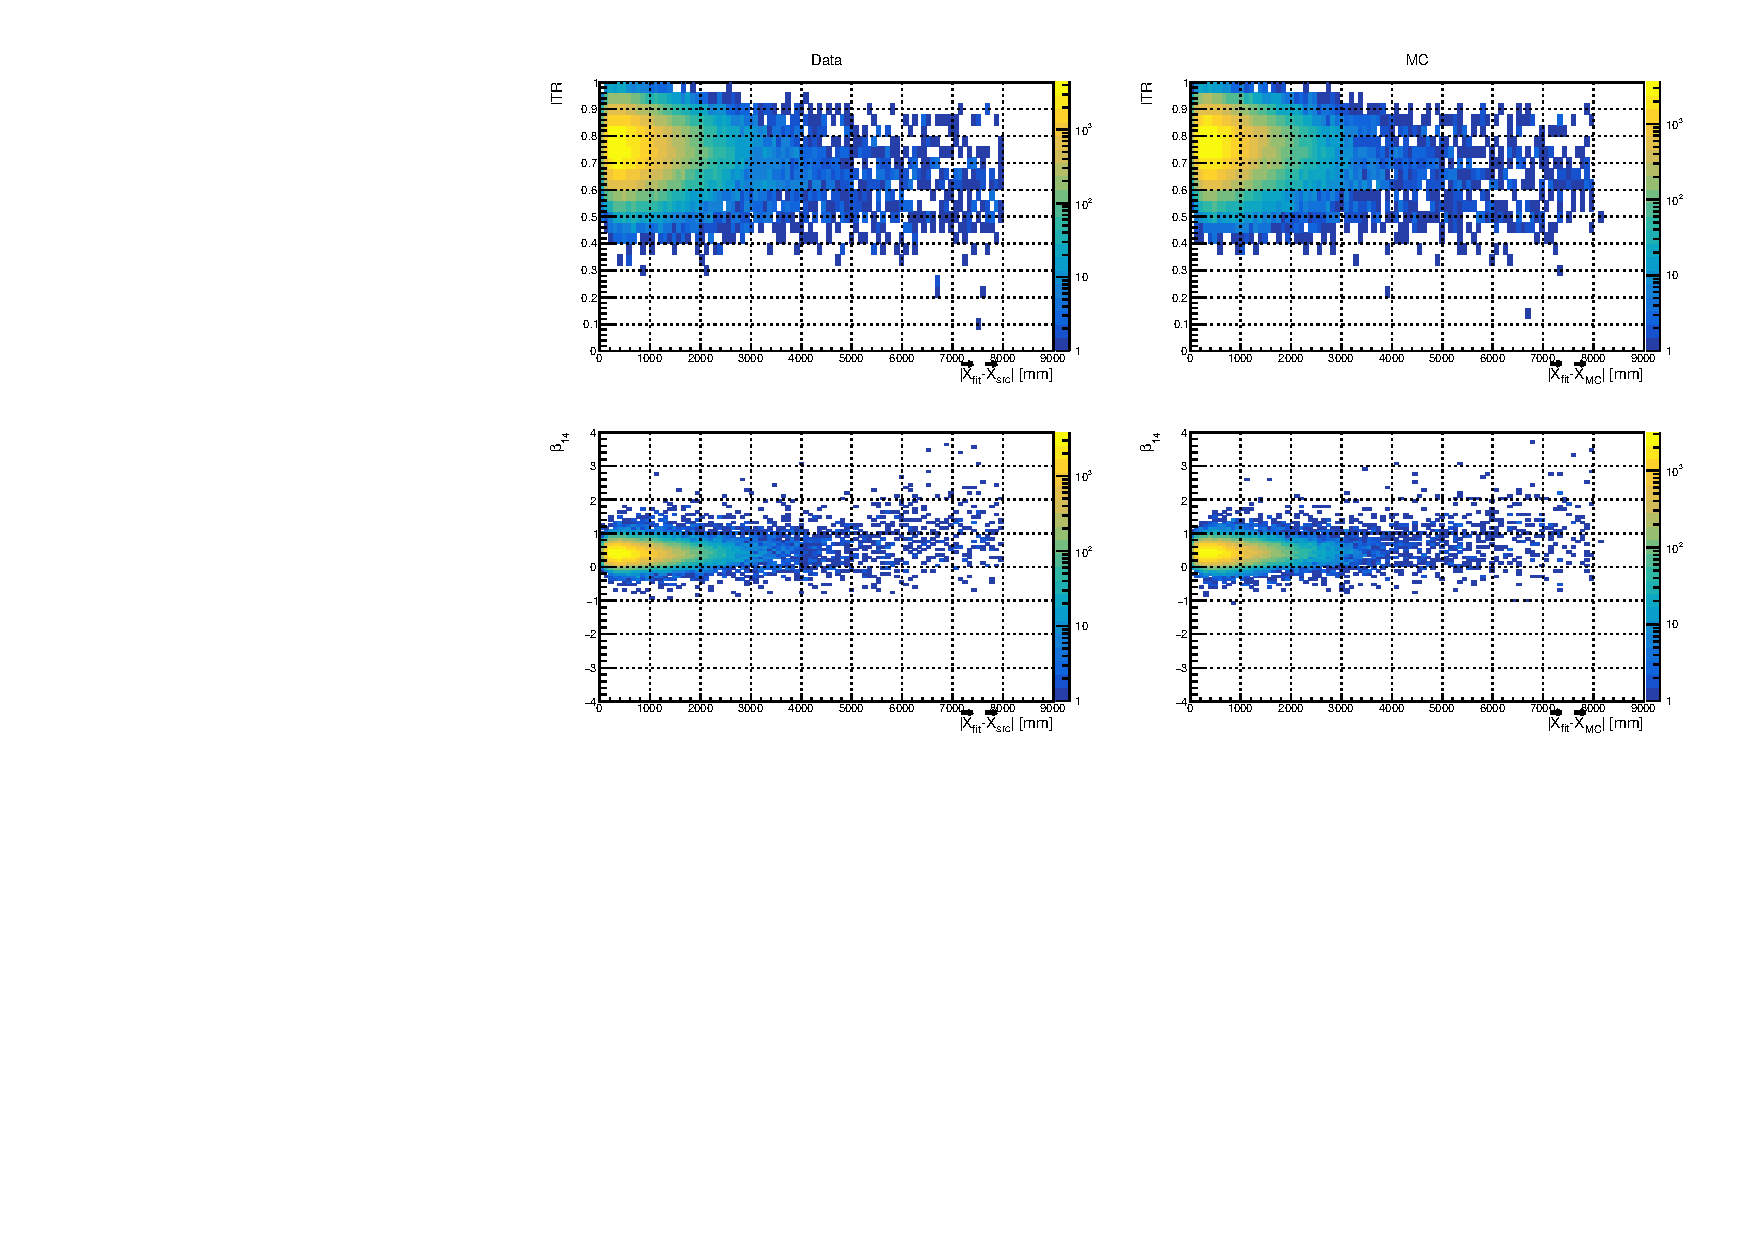
\includegraphics[width=14cm]{N16_107055_highLevelCuts.pdf}
	\caption[Position biases vs $ITR$ (top) and $\beta_{14}$ (bottom) for the $^{16}$N central run-107055.]{Position biases vs $ITR$ (top) and $\beta_{14}$ (bottom) for the $^{16}$N central run-107055. Left is MC and right is data. For the data, the source position ($\vec{X}_{src}$) was compared.}
	\label{n16_highLevelCut}
\end{figure}

As a summary, the high-level cuts remove more than half of the events with large position biases while removes about 1.6\% of the total events. 

\section{Reconstruction Evaluations from $^{16}$N Calibration Scans in the Water Phase}

In this section, by analyzing the $^{16}$N data and MC in the water phase, I extracted the reconstruction resolutions of the event position, direction, and energy respectively. Then by comparing the data with the MC, the reconstruction systematics were evaluated.

To do these evaluations, a few cuts were applied to both the data and MC. Firstly, the level cuts  ($ITR>0.55$, $-0.12<\beta_{14}<0.95$) were applied. For events with the position, direction and energy successfully reconstructed (i.e., the event has valid position, direction and energy reconstructions), further cuts on the reconstruction figure of merit (FoM) and source geometry (will be described in detail) were applied to ensure that the analyzed events were nicely reconstructed physics events caused by the source $\gamma$ particles interacting with the detector water.

\subsection{Position Reconstruction Evaluation}
The position figure of merit (posFoM) cuts mentioned in Sect.~\ref{sect:positinFoM} were applied on the reconstruction results. Fig.~\ref{posBiasVsFOM} shows the $scaleLogL$ with the position biases for the reconstructed events in $^{16}$N central calibration run-107055. Both of the data and the MC simulations are shown. For the MC case, the position biases are between the reconstructed positions and the true positions generated by the MC: $|\vec{X}_{fit}-\vec{X}_{MC}|$; while for the data case, the biases are between the reconstructed positions and the source manipulation position: $|\vec{X}_{fit}-\vec{X}_{src}|$.

\begin{figure}
	\centering
		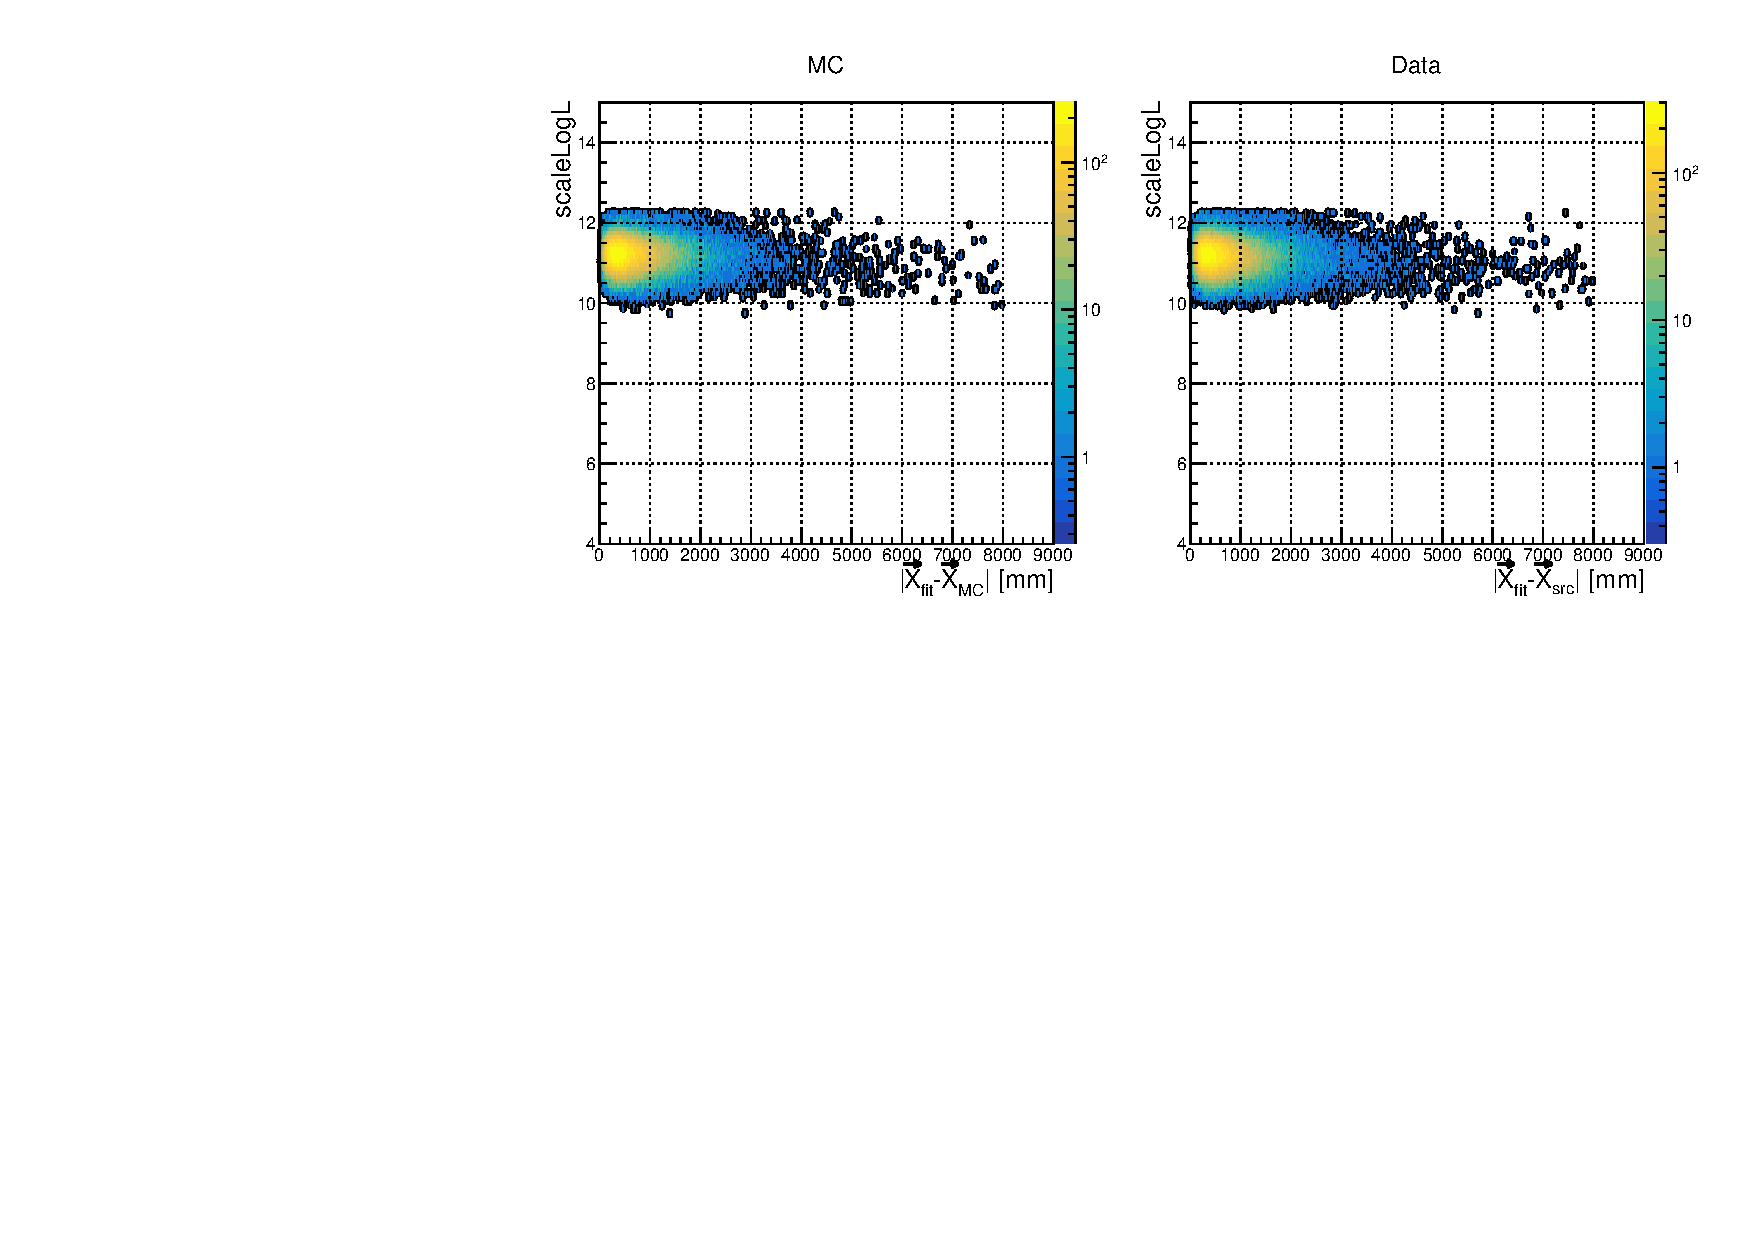
\includegraphics[width=13cm]{N16_107055_scaleLogLvsPosBias.pdf}
	\caption[Position biases ($|\vec{X}_{fit}-\vec{X}_{MC}|$) vs $scaleLogL$ for the $^{16}$N central run-107055.]{Position biases ($|\vec{X}_{fit}-\vec{X}_{MC}|$) vs $scaleLogL$ for the $^{16}$N central run-107055. Left is MC and right is data. For the data, the source position ($\vec{X}_{src}$) was compared.}
	\label{posBiasVsFOM}
\end{figure}

For the MC (data) case, about 0.035\% (0.043\%) of the total reconstructed events have large biases ($|\vec{X}_{fit}-\vec{X}_{MC}|>6000$ mm). A cut of $scaleLogL>10$ removes 96.0\% (97.3\%) of the events which have biases over 6000 mm, with a sacrifice of removing 0.012\% (0.016\%) of the total events.

Fig.~\ref{energyVsFOM} shows a relation between the $scaleLogL$ and the reconstructed energy ($E_{fit}$). 

For the events with reconstructed energies below the water solar neutrino analysis threshold 3.5~MeV ($E_{fit}<3.5~MeV$), they are mostly coming from the U/Th isotopes, decays of Potassium as well as instrumental noises\cite{waterunidoc}. Their lower energies or $NHits$ can affect the position reconstruction since there are fewer PMTs to be used, and thus their $posFoM$ can be worse.
In the MC (data) case, there are about 13.04 \% (12.89\%) of the events with $E_{fit}<3.5~MeV$. By applying the cut of $scaleLogL>10$, 0.10\% (0.09\%) of such events were removed.

\begin{figure}[!htb]
	\centering
	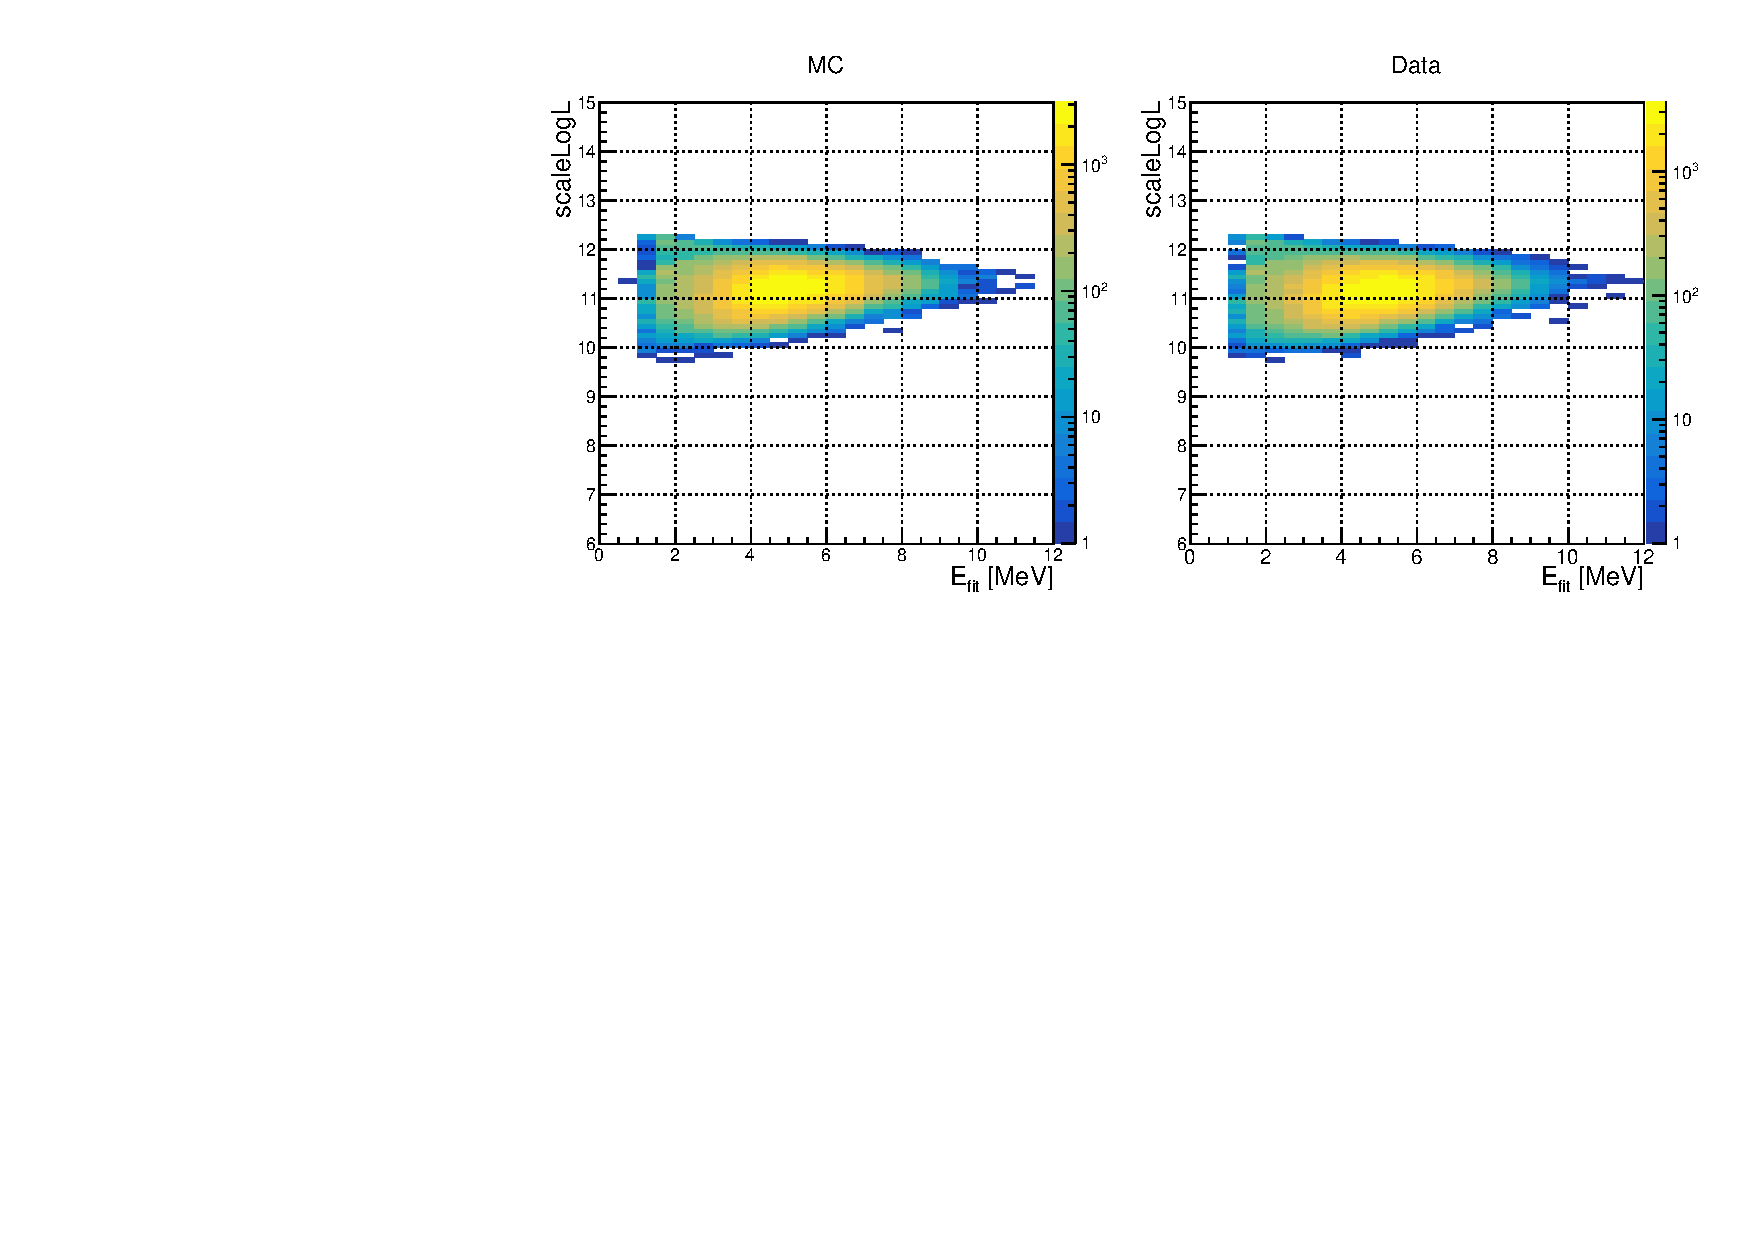
\includegraphics[width=13cm]{N16_107055_scaleLogLvsEnergy.pdf}
	\caption{Reconstructed energy vs $scaleLogL$ for the $^{16}$N central run-107055. Left is MC and right is data.}
	\label{energyVsFOM}
\end{figure}

As a summary, there are about 0.04\% of the reconstructed events which were poorly reconstructed (mis-reconstructed) by the \texttt{MPW fitter} with position biases over 6 meters. Applying a cut in $posFoM$ with $scaleLogL>10$ can remove over 96\% mis-reconstructed events. This $posFoM$ cut was used in the following direction and energy reconstruction evaluations.

\subsubsection{Position Resolution}
A position resolution function is defined for the reconstructed electron position distribution\cite{boulay2004direct}:
\begin{equation}
R(x)=\frac{1-\alpha_e}{\sqrt{2\pi}\sigma_p}\exp{[-\frac{1}{2}(\frac{x-\mu_p}{\sigma_p})^2]+\frac{\alpha_e}{2\tau_p}\exp{[\frac{-|x-\mu_p|}{\tau_p}]}},
\end{equation}
where $\alpha_e$ is the fractional exponential component, $\sigma_p$ is
the Gaussian width (corresponding to the position resolution), $\mu_p$ is the Gaussian shift (corresponding to the position bias) and $\tau_p$ is the exponential slope (corresponding to the position distributions in tails).

The $\gamma$-rays emitted from the $^{16}$N source interact with the water in the detector mainly via Compton scattering, as shown in Fig.~\ref{N16centralDiagram}. The position distribution of the $\gamma$ interaction vertices is peaked around the source container, spreading to about 2 meters.

\begin{figure}[!htb]
	\centering
	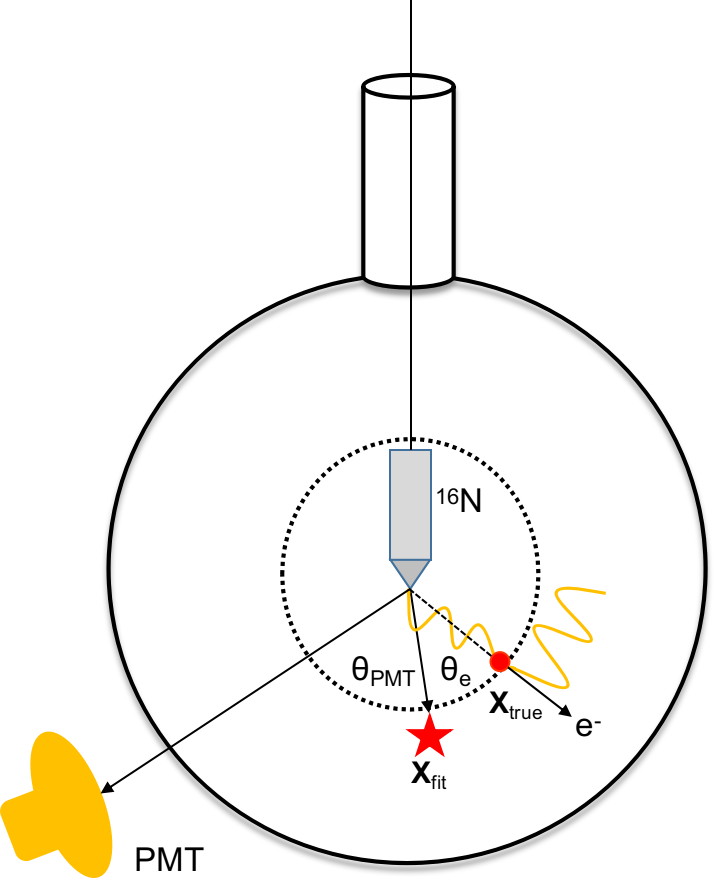
\includegraphics[width=8cm]{N16centralDiagram.png}
	\caption{A cartoon shows the $^{16}$N source.}
	\label{N16centralDiagram}
\end{figure}

Fig.~\ref{hsx} shows the spatial distributions $S(x)$ of the first $\gamma$-ray interaction positions projected on the x-axis obtained from MC simulation. Therefore, the $^{16}$N source is considered as an electron source with a known spatial distribution\cite{boulay2004direct}. For simplicity, in the following, we always discuss the $x$ component of the position vector $\vec{X}$. 

\begin{figure}[!htb]
	\centering
	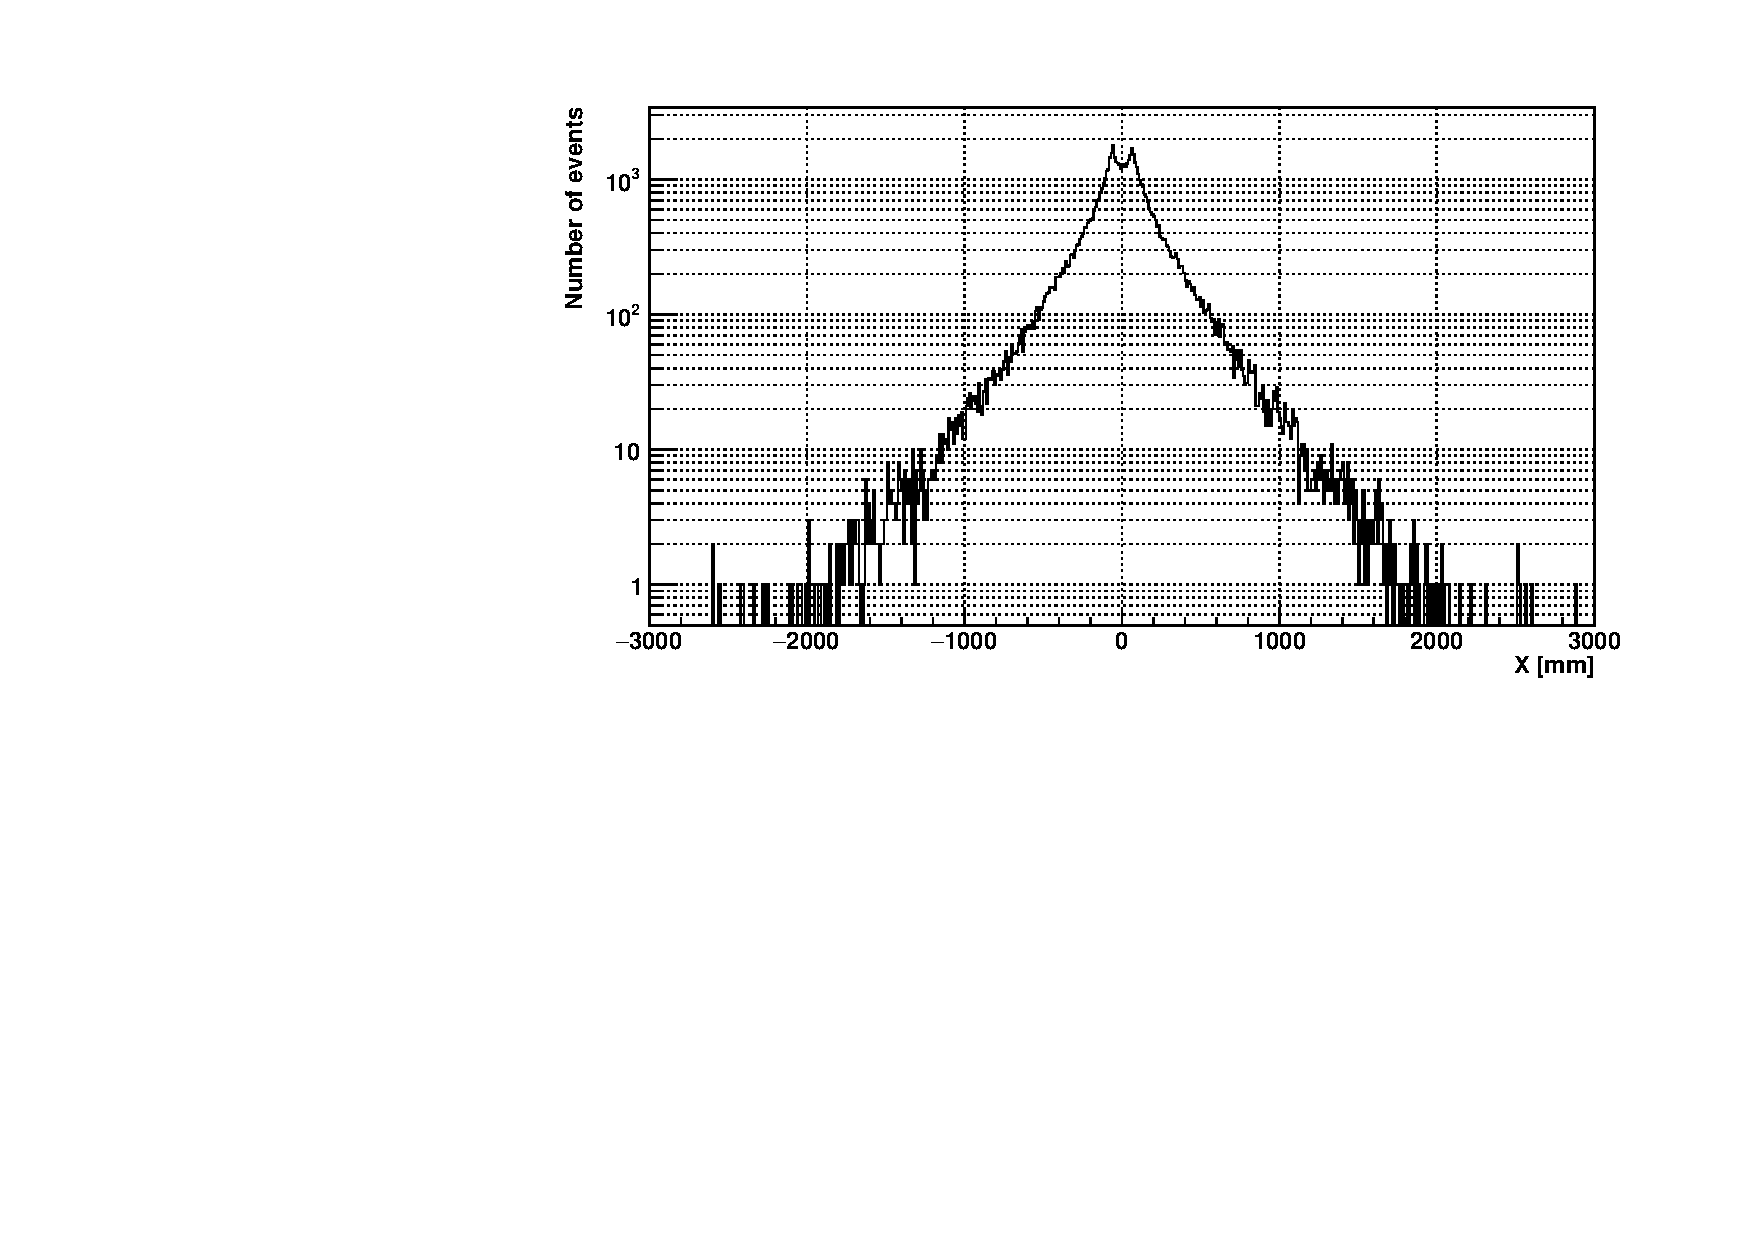
\includegraphics[width=12cm]{sx.pdf}
	\caption[Spatial distributions of {$^{16}$}N first $\gamma$-rays interaction position projected on x axis.]{Spatial distributions of {$^{16}$}N first $\gamma$-rays interaction position projected on x axis, obtained from the \texttt{RAT} simulations. The double-peak structure is due to the wall of the stainless steel container of the $^{16}$N source.}
	\label{hsx}
\end{figure}

For electrons from the $^{16}$N calibration source, their spatial distribution function $N_{R}(x)$ can be described by the position resolution function smeared by the convolution of $S(x)$ as\cite{boulay2004direct}:
\begin{equation}
N_{R}(x)=\int^{+\infty}_{-\infty} S(x)R(x_{fit}-x)dx,
\end{equation}

The values of $N_{R}(x)$ can be calculated bin by bin from the histograms of $S(x)$ and $R(x)$ extracted from the MC or data: 
\begin{equation}
N_R(x_i)=\sum_{x_i=-\infty}^{+\infty}S(x_i)R(x_{fit}^i-x_i),
\end{equation}

Then the $\chi^2$ is calculated by:
\begin{equation}
\chi^2=\sum^{N_{bins}}_{i=0}[\frac{N_R(x_{fit}^i)-N_R^{fit}(x_{fit}^i)}{\sigma_i}]^2,
\end{equation}
where $N_R^{fit}$ is a trial fit to the $N_R$ by tuning the $\{\alpha_e,\mu_p,\sigma_p,\tau_p\}$ and $\sigma_i$ is taken as the bin width of the histograms.

By minimizing the $\chi^2$, the parameters of the resolution function, $\{\alpha_e,\mu_p,\sigma_p,\tau_p\}$ and a best $N_R^{fit}$ were obtained.

Fig.~\ref{fig:posresol} shows a comparison of the reconstructed x position of {$^{16}$}N events between data and MC. The reconstructed position distributions were fitted with $N_R^{fit}$.

\begin{figure}
	\centering
	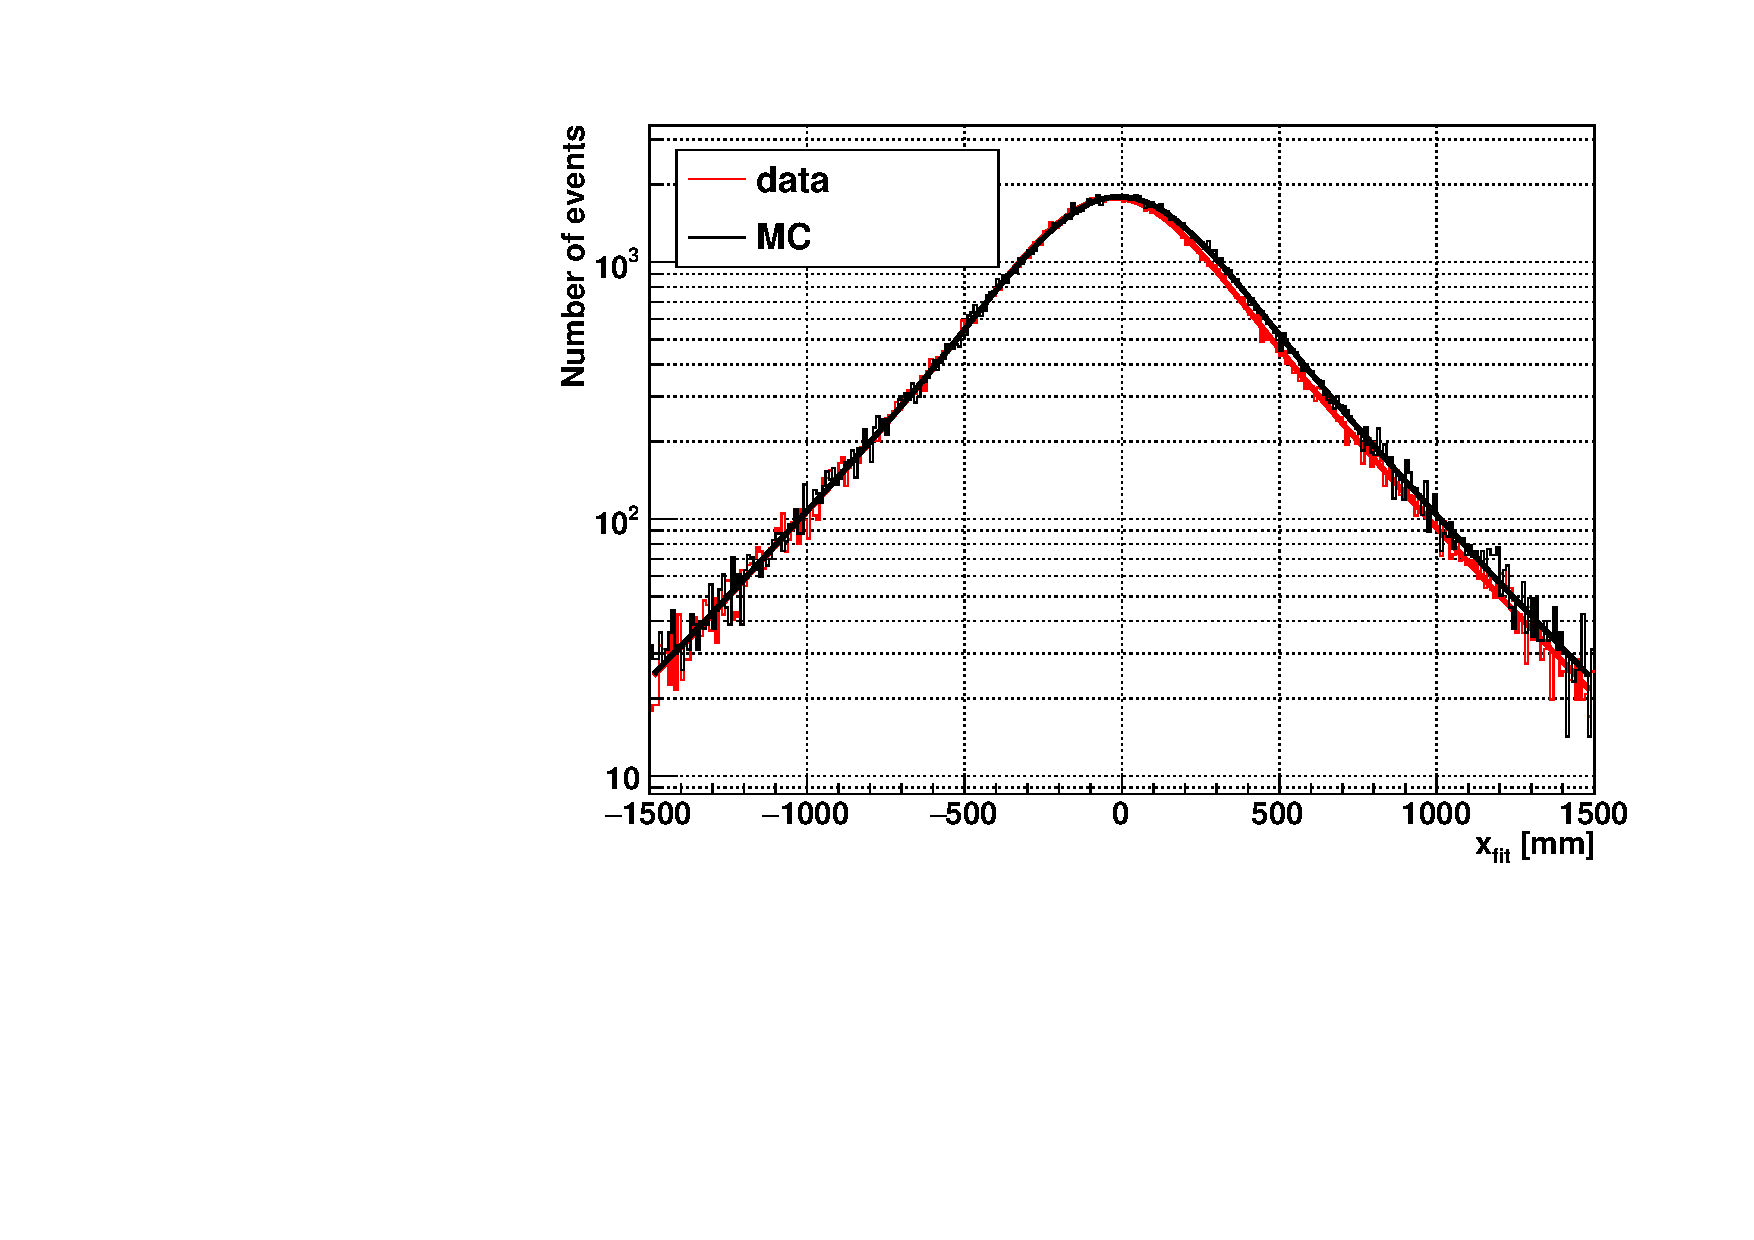
\includegraphics[width=140mm]{posResol.pdf}
	\caption[Distributions of the reconstructed position projected on x axis.]{Distributions of the reconstructed position projected on x axis, obtained from SNO+ {$^{16}$}N central run data (red) and MC (black). The distributions are fitted with $N_R^{fit}$ (red and black lines).}
	\label{fig:posresol}
\end{figure}

Table.~\ref{tab:posresol} summarizes the values of position resolution parameters (for x-axis) obtained from data and MC of {$^{16}$}N calibration runs at the detector center.
\vspace{1mm}
\begin{table}[ht]
	\centering
	\caption{Position resolution parameters for the \texttt{MPW fitter} (x-axis).}
	\label{tab:posresol}
	\begin{tabular}{ccccc}
		\toprule
		MPW fitter & $\alpha_e$ & $\sigma_P$ (mm) &  $\tau_P$ (mm)& $\mu_P$ (mm)\\
		\hline 
		data& 0.58$\pm$0.04 & 175.8$\pm$3.8 & 288.0$\pm$5.7 & -28.8$\pm$1.0\\	
		\hline 
		MC & 0.51$\pm$0.05 & 195.2$\pm$3.3 & 298.4$\pm$6.1 & -10.9$\pm$1.0\\
		\bottomrule
	\end{tabular}
\end{table}
\vspace{1mm}

\subsubsection{Position Systematics}
To evaluate the position uncertainties, the MC and data runs of the $^{16}$N internal scans along x, y, z axes were taken to evaluate the x, y, z position uncertainties respectively (the runs are listed in Table.~\ref{table:n16scanTable_zscan} to ~\ref{table:n16scanTable_xscan}. Three neck runs in z-scan were not used). The high-level cuts as well as the $E_{fit}>3.5~MeV$ and $scaleLogL>10$ cuts were applied. 
fit range was set as $[-2000, +2000]~mm$. If the lower range was smaller than -6000~mm, it was set to -6000~mm; if the upper range was larger than 6000~mm, it was set to +6000~mm. This was used to remove the effects caused by the AV.

The position resolution function was first fitted with 4 free parameters: $\alpha_e,\mu_p$, $\sigma_p$ and $\tau_p$. The the average values of the $\alpha_e$
and $\tau_p$ were calculated from all the scan runs used here. To simplify the calculation in propagating systematics, the $\alpha_e$ and the $\tau_p$ were fixed to the average value: $\alpha_e=0.5288$ (0.5375) for the MC (data); $\tau_p=271.738$ (263.735) for the MC (data). With the fixed values of $\alpha_e$ and $\tau_p$, both the data and the MC were refit with $\mu_p$ and $\sigma_p$ only. Using the fixed values of $\alpha_e$ and the $\tau_p$ is based on the reasons that these parameters in principle can be viewed as corrections to the $\gamma$ distribution ($S(x)$) and they can be absorbed, which would not depend on position\cite{waterunidoc}. 

Fig.~\ref{MPWscanXYZResols} shows the fitted results of $\mu_P$ and $\sigma_P$ along the x, y, z-axes scans respectively. For the sake of simplicity, for the x-scan case, only the x-axis results ($\mu_{P,x},\sigma_{P,x}$) are shown here. Similarly, only the $\mu_{P,y}$ and $\sigma_{P,y}$ ($\mu_{P,z}$ and $\sigma_{P,z}$) are shown for the y-scan (z-scan). The relative differences discussed later consider all the three axes.

\begin{figure}
	\centering
	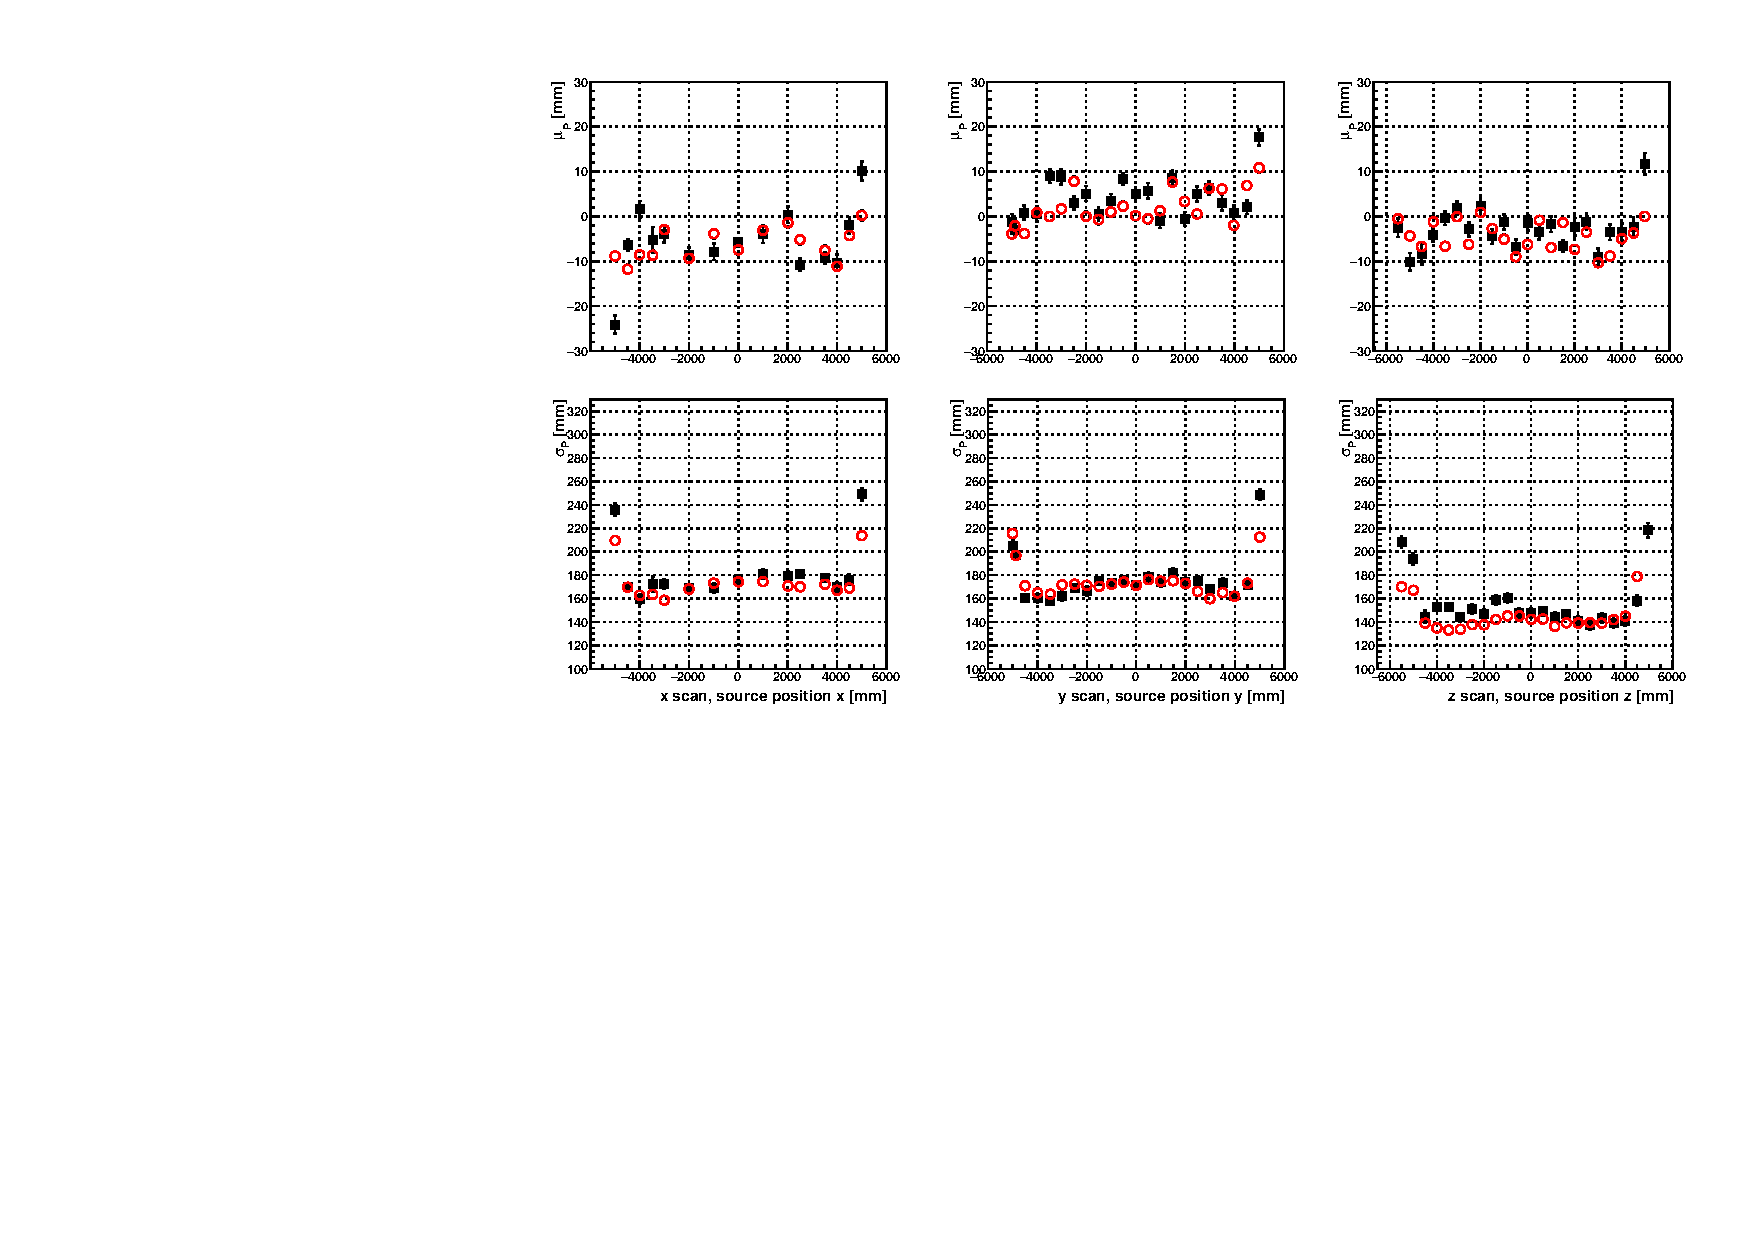
\includegraphics[width=16cm]{N16_rat6176_muPandSigmaP_xyzScans.pdf}
	\caption[The fitted values of $\mu_P$ and $\sigma_P$ along x, y and z scans.]{The fitted values of $\mu_P$ (top) and $\sigma_P$ (bottom) along x (left), y (middle) and z (right) scans. The source positions in each set of scans are projected onto x, y and z axes respectively. The MC results (red circles) are compared with the data (black boxes).}
	\label{MPWscanXYZResols}
\end{figure}

It shows that the position resolutions of the MC are mostly better than the data, which is expected since the non-uniformities of the detector in realistic situations can cause a broader resolution in the data\cite{waterunidoc}. Also, when the source is close to the AV or at the edges of the axes, the Gaussian shift $\mu_P$ becomes large and the resolution worsens. Also, the difference between the MC and data becomes large.

To quantify the discrepancies between the MC and data, a relative difference of $\sigma_p$ between the MC and data is defined as\cite{waterunidoc}:
\begin{equation}
\sigma_{p,\delta}\equiv\sqrt{\sum_i|(\sigma^{data}_{P,i})^2-(\sigma^{MC}_{P,i})^2|}~~(i=x,y,z),
\end{equation}
 
Fig.~\ref{pos_relative_sigma_biasesVsPositions} shows the $\sigma_{p,\delta}$ changing along the internal x, y and z-axes scans respectively. All the differences are below $190~mm$ except the run-106979 with the source at $z=4973.567~mm$. The neck effects can cause this worst resolution. 

It goes worse when the source is close to the AV or at the edges of the axes. When the source is close to the AV center, the differences are below $100~mm$.

\begin{figure}[!htb]
	\centering
	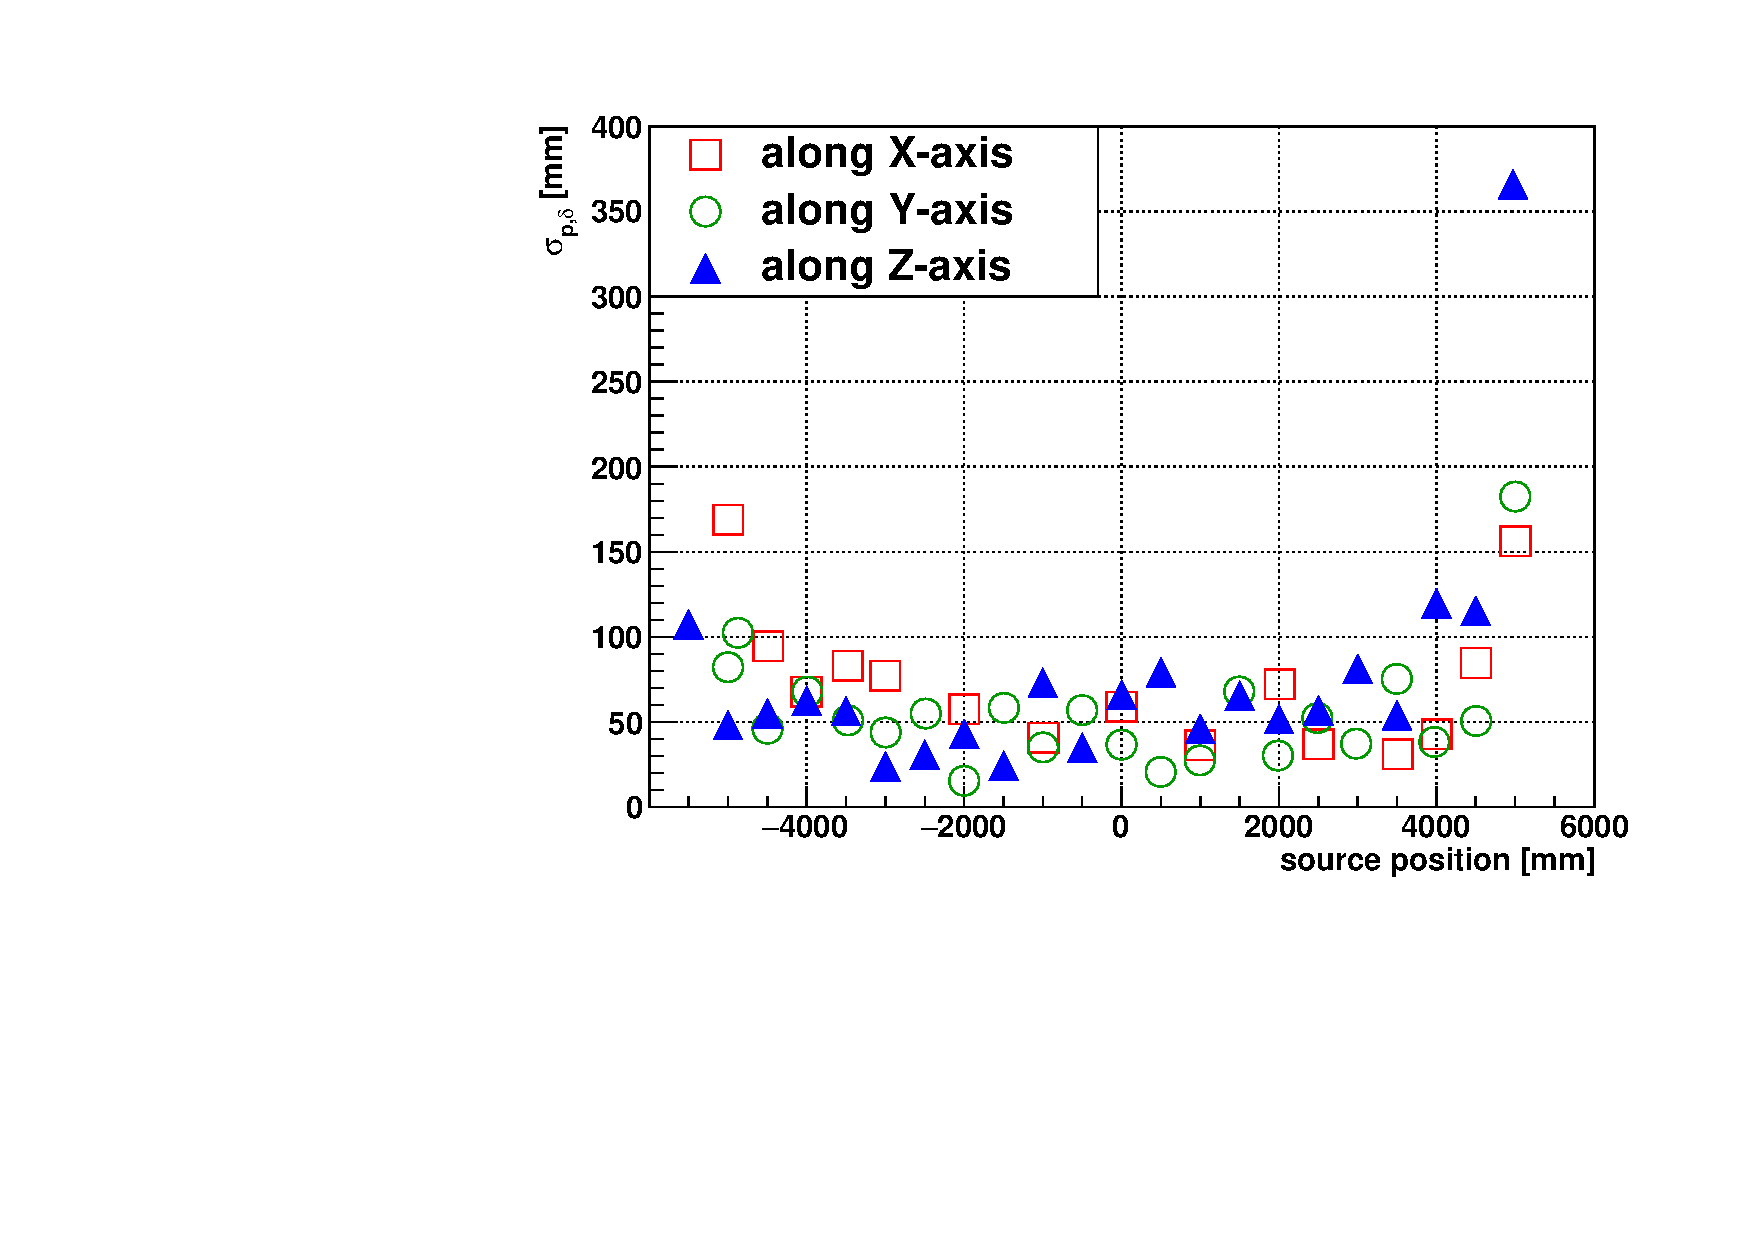
\includegraphics[width=16cm]{N16_6176_pos_sigmaP_data_mc.pdf}
	\caption[Relative differences of $\sigma_P$ ($\sigma_{p,\delta}$) as a function of the $^{16}$N source position.]{Relative differences of $\sigma_P$ ($\sigma_{p,\delta}$) as a function of the $^{16}$N source position. For simplicity, the corner scans are not shown in this figure. The red squares represent the results from the x-scan runs; green circles represent the y-scan runs and the blue triangles represent the z-scan runs.}
	\label{pos_relative_sigma_biasesVsPositions}
\end{figure}

The values of $\sigma_{p,\delta}$ were taken to represent the position resolution systematics.

As listed in Table.~\ref{vertexResolsSys}, the averages and the standard deviations of the $\sigma_{p,\delta}$ were taken as the resolution systematics for x, y and z-axes respectively. To smear the position results, a Gaussian distribution $\mathcal{N}(0,\delta)$ was convolved with positions. The upper values $\delta$ were used to smear the positions.
\begin{table}[ht]
	\centering
	\caption{The \texttt{MPW fitter} position resolution systematic uncertainties in x, y and z axes. Unit: mm.}
	\vspace{3mm}
	\label{vertexResolsSys}
	\begin{tabular*}{140mm}{c@{\extracolsep{\fill}}ccc}
		\toprule
		axis & systematic uncertainties & systematic to be applied ($\delta$) &smearing\\
		\hline 
		x  & $73.89\pm39.71$ & 113.6 & $x+\mathcal{N}(0,\delta)$\\
		y  &  $56.03\pm34.96$ & 90.99 & $y+\mathcal{N}(0,\delta)$\\
		z   & $75.47\pm70.09$ & 145.56& $z+\mathcal{N}(0,\delta)$\\
		\bottomrule
	\end{tabular*}
\end{table}

To quantify the vertex shifts between the MC and data, values of vertex shifts: $\mu_{P,\delta}\equiv\mu_P(data)-\mu_P(MC)$ were calculated for the x, y and z scans respectively. Fig.~\ref{fig:verteshitfs} shows these results.
\begin{figure}[!htb]
	\centering
	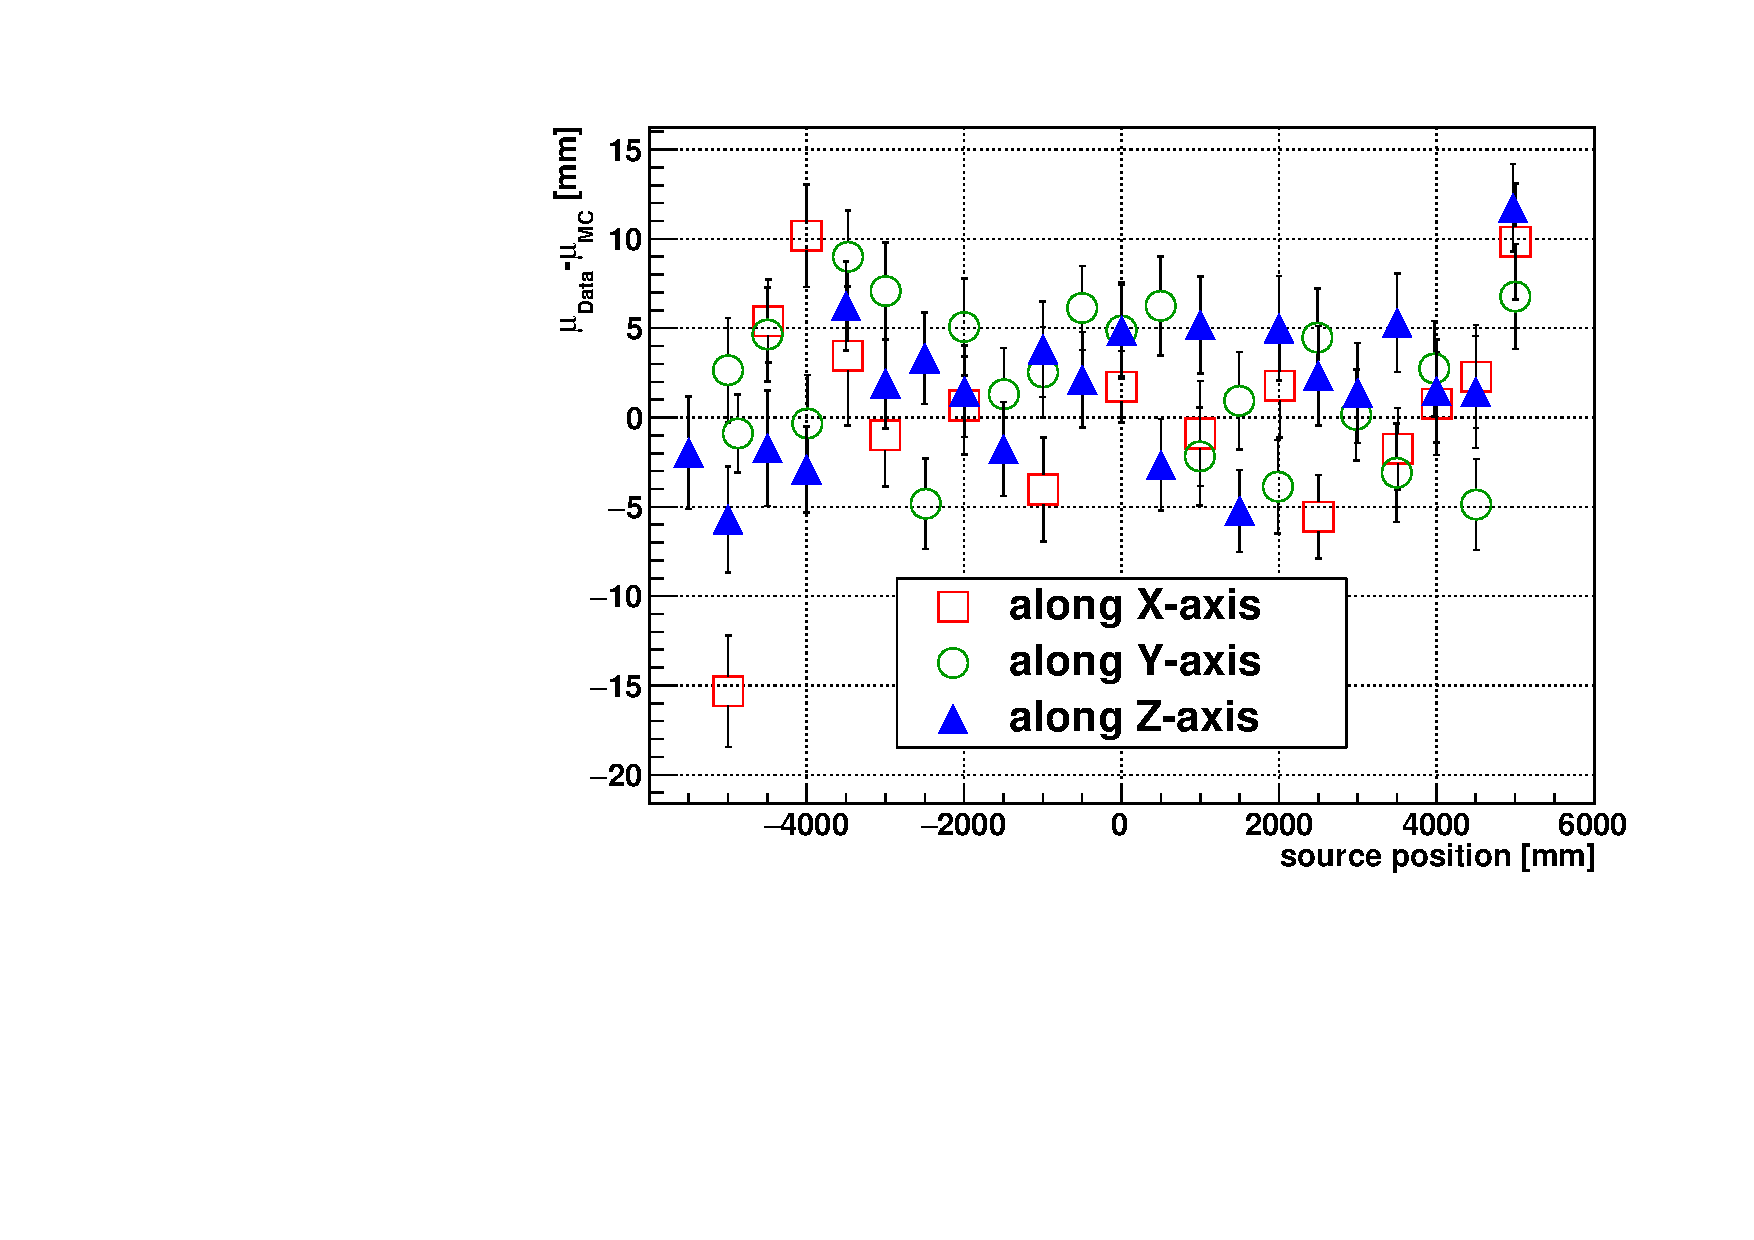
\includegraphics[width=16cm]{N16_rat6176_vertexShift_xyzScans.pdf}
	\caption[Vertex shifts of $\mu_P$ ($\mu_{p,\delta}$) as a function of the $^{16}$N source position.]{Vertex shifts of $\mu_P$ ($\mu_{p,\delta}$) as a function of the $^{16}$N source position. For simplicity, the corner scans are not shown in this figure. The red squares represent the results from the x-scan runs; green circles represent the y-scan runs and the blue triangles represent the z-scan runs.}
	\label{fig:verteshitfs}
\end{figure}

In Table.~\ref{vertexShifts}, the averages and the standard deviations of the $\mu_{P,\delta}$ were taken as the vertex shifts for x, y and z-axes respectively. To smear the position results, the positions were simply shifted by the upper values $\delta$ were used to smear the positions.
\begin{table}[ht]
	\centering
	\caption{Vertex shifts for the reconstructed positions in x, y and z axes. Unit: mm.}
	\vspace{3mm}
	\label{vertexShifts}
	\begin{tabular*}{120mm}{c@{\extracolsep{\fill}}cccc}
		\toprule
		axis & vertex shift  & systematic to be applied ($\delta$) &smearing\\
		\hline 
		x shift &  0.50$\pm$5.98 & +6.48/-5.98 & $x+\delta$\\	
		y shift  & 2.02$\pm$4.11 & +6.13/-4.11 & $y+\delta$\\
		z shift & 1.89$\pm$4.82 & +6.71/-4.82 & $z+\delta$\\
		\bottomrule
	\end{tabular*}
\end{table}

\subsubsection{Vertex Scale Uncertainties}
In addition to the vertex shifts mentioned previously, the vertex scale is defined as a linear scale factor between the fitted positions of the data and the MC: $x^{data}_{fit}-x^{MC}_{fit}=\mu^{data}_{P,x}-\mu^{MC}_{P,x}=\Delta+\beta\cdot x^{MC}_{fit}$.

Since $x^{data}_{fit}=\Delta+(1+\beta)\cdot x^{MC}_{fit}$, if the vertex scale factor is defined as: $\alpha\equiv 1+\beta$, then $x_{data}=\alpha x_{MC}$.

To obtain the $\alpha$, the results in Fig.~\ref{fig:verteshitfs} were fitted with linear functions: $shifts = p_0+p_1\cdot x_{src}$ (where $x_{src}$ is the source position), as shown in Fig.~\ref{fig:vertexScale}.

\begin{figure}
	\centering
	\subfigure[$^{16}$N x-scan runs.]{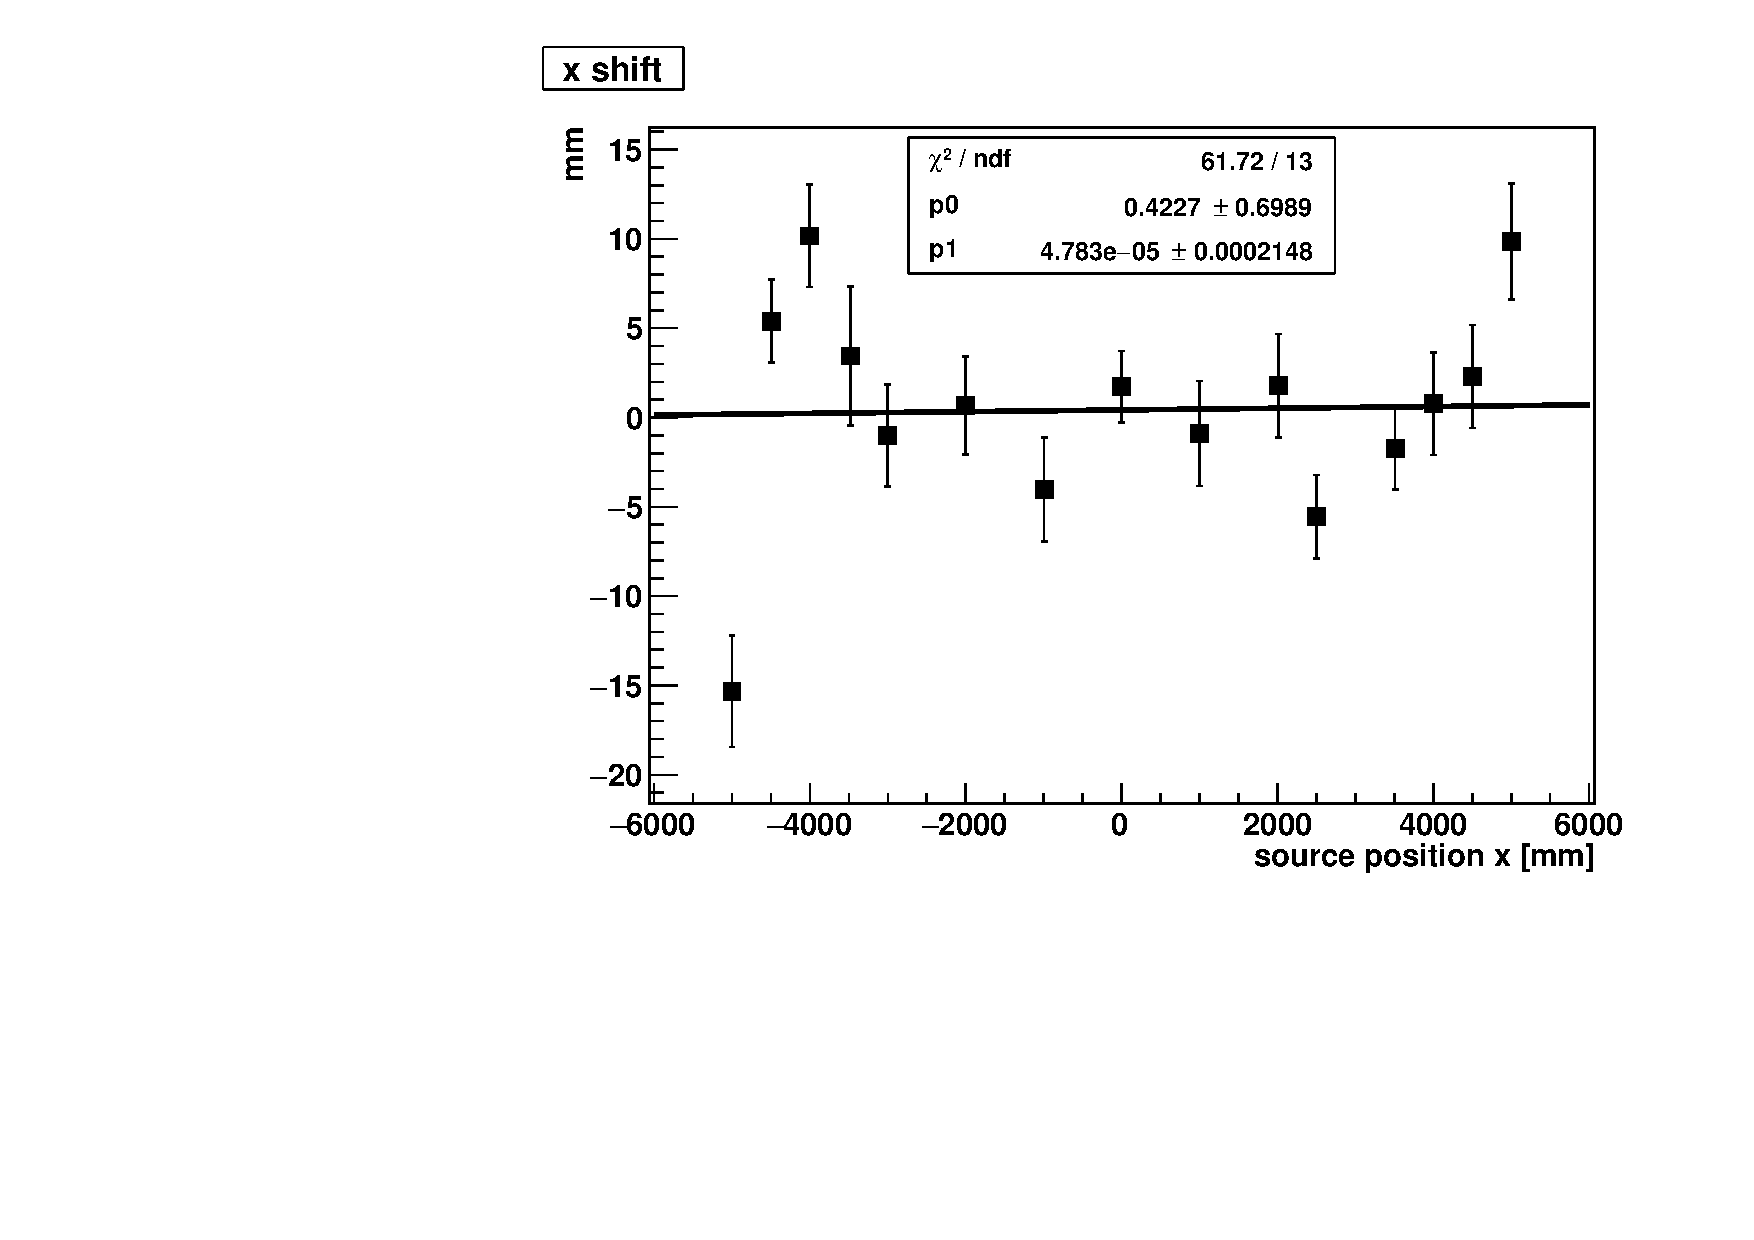
\includegraphics[width=5cm]{vertexScaleSysX.pdf}}
	\subfigure[$^{16}$N y-scan runs.]{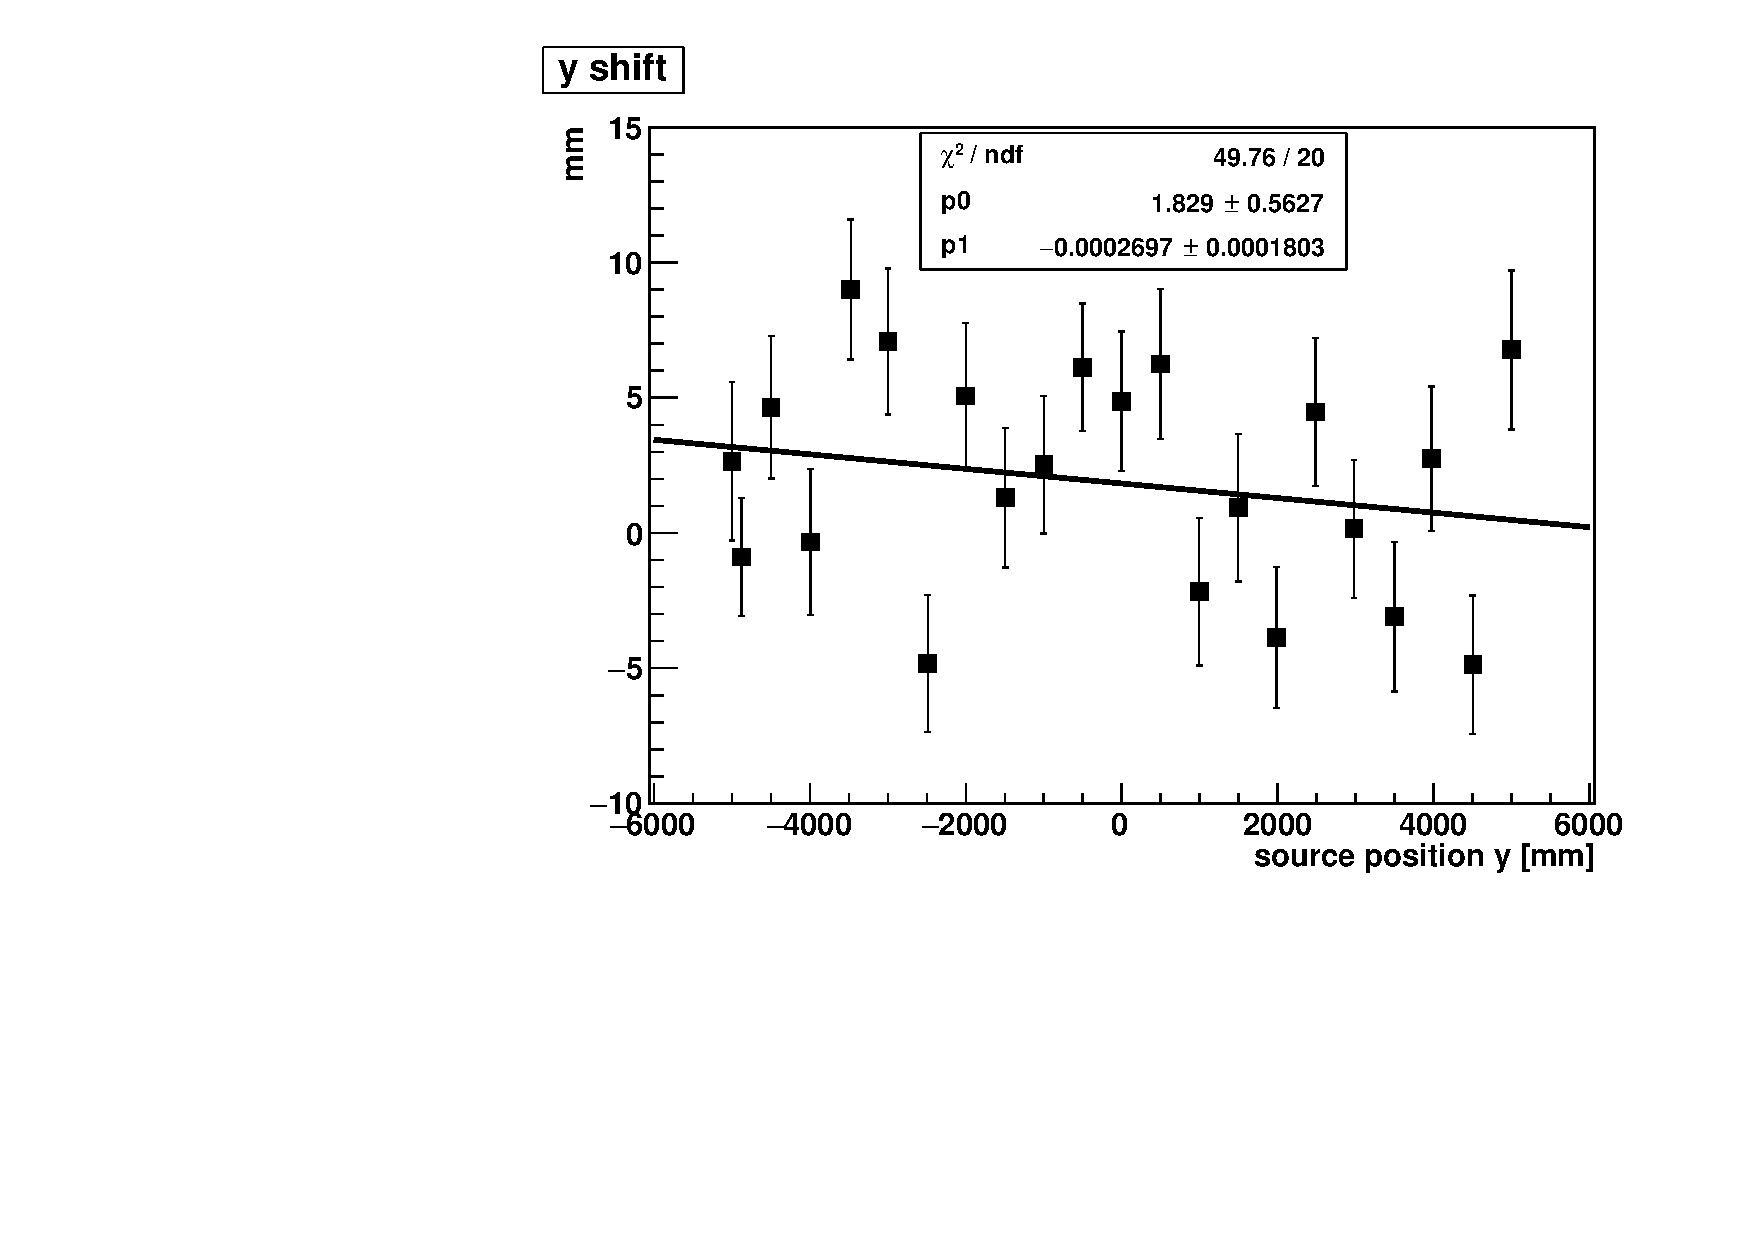
\includegraphics[width=5cm]{vertexScaleSysY.pdf}}
	\subfigure[$^{16}$N z-scan runs.]{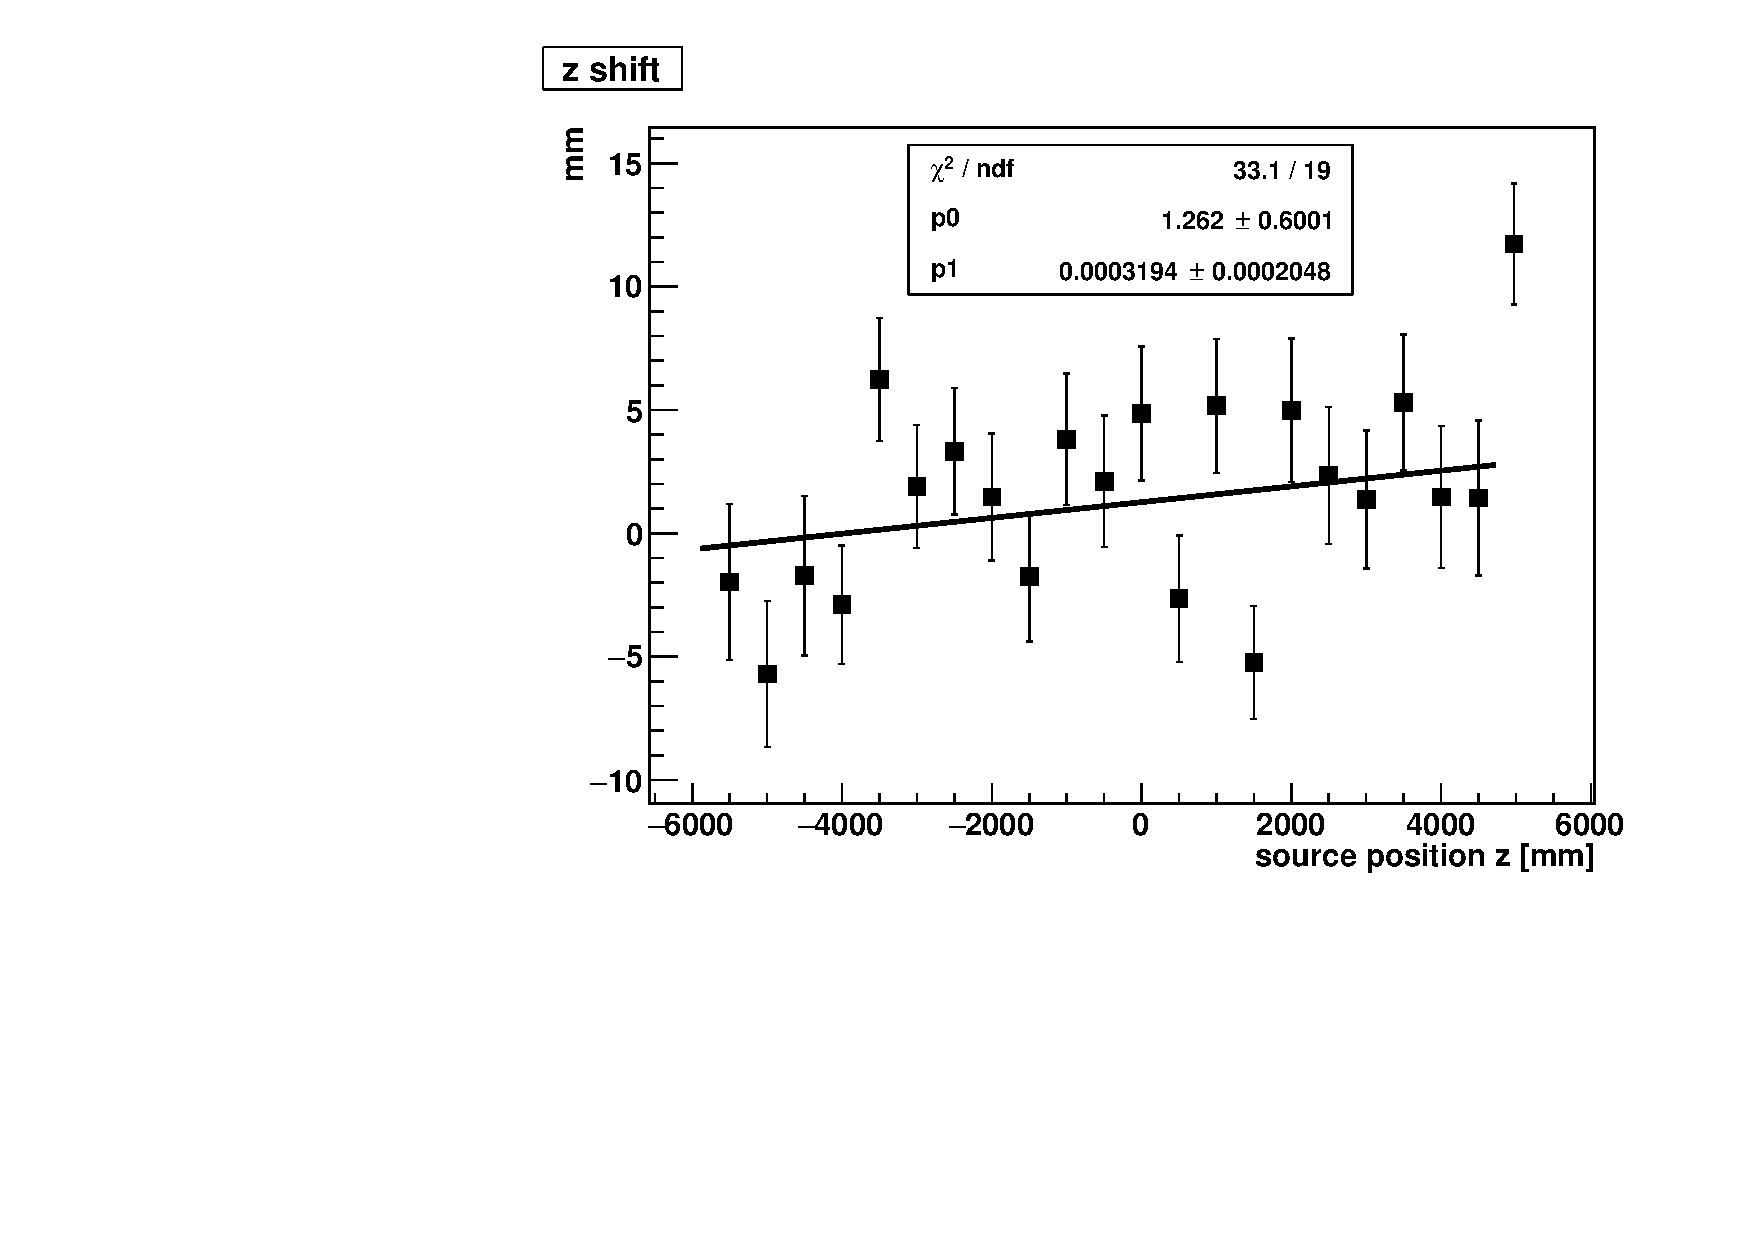
\includegraphics[width=5cm]{vertexScaleSysZ.pdf}}
	\caption{Vertex shifts along x, y, z axes and fitted with linear functions.}
	\label{fig:vertexScale}
\end{figure}

From the linear fits, the values of vertex shifts were obtained and listed in Table.~\ref{table:vertexScale}. Since the $\chi^2/ndf$ values here were large, according to Refs.~\cite{waterunidoc,pdg2020}, inflated errors were calculated as $S\times$(slope errors), where the error scale factor $S=\sqrt{\chi^2/(ndf-1)}$. The downward systematic was calculated as the slope minus the slop error as well as the inflated error. In contrast, the upward systematic was taken as the positivel inflated error, as suggested by \cite{waterunidoc}. For the z scan, the position at $(-185.037,247.24,4973.567)$ mm pulls the slope results to the positive due to the possible biases in simulation for the neck geometry effects and makes the slope positive. So this point was not used in the linear fit.

\begin{table}[ht]
	\centering
	\caption{Vertex shifts for the reconstructed positions in x, y and z axes. Unit: mm.}
	\vspace{2mm}
	\label{table:vertexScale}
	\begin{tabular*}{130mm}{c@{\extracolsep{\fill}}cccc}
		\toprule
		axis & fitted slope (\%)  & inflated error &systematic ($\delta^+/\delta^-$) (\%)\\
		\hline 
		x scale &  0.005$\pm$0.021 & 0.048 & +0.07/-0.06\\	
		y scale  & -0.027$\pm$0.018 & 0.030&  +0.02/-0.07\\
		z scale & 0.032$\pm$0.020 & 0.027&  +0.08/-0.01\\
		\bottomrule
	\end{tabular*}
\end{table}

The vertex scale systematics is then transformed by:
$x'=(1+\delta_x/100)x$, the same for $y,z$.

The scale systematics also depends on the radius $r=\sqrt{x^2+y^2+z^2}$\cite{waterunidoc}. By the error propagation, for an event position (x,y,z), $\delta_r$ is calculated as\cite{waterunidoc}:
\begin{equation}
\delta_r =\sqrt{\sum_{i=1}^3(\frac{\partial r}{\partial x_i})^2\delta^2_{x_i}}= \sqrt{\frac{x^2\delta_x^2+y^2\delta_y^2+z^2\delta_z^2}{r^2}},
\end{equation}

where the $\delta^+_r$ and $\delta^-_r$ are calculated by $\delta^+$ and $\delta^-$ respectively.

Then the two-sided bounds of the radial $r$ are calculated by:
$r^+=(1+\delta^+_r/100)\cdot r$ and $r^-=(1+\delta^-_r/100)\cdot r$.

%Uncertainties from the source manipulator positions are assumed to be 50~mm.

\subsection{Direction Reconstruction Evaluation}
\subsubsection{Direction Resolution}
For the reconstructed events in the $^{16}$N calibration, assuming a $\gamma$ particle emitted from the source and interacts with $e^-$ at the reconstructed position, the ``true'' direction of an event is defined as the direction pointing from the source manipulation position to the reconstructed position: $\vec{u}_{true} = (\vec{X}_{fit}-\vec{X}_{src})/|\vec{X}_{fit}-\vec{X}_{src}|$. The angle $\theta$ is the displacement between the ``true'' and the reconstructed directions and $\cos\theta=\vec{u}_{true}\cdot \vec{u}_{fit}$.

The distribution of the $\cos\theta$ was fitted with the direction resolution function (Eqn.~\ref{eq:directResol}) mentioned in Sect.~\ref{sect:directResol}, Chapter 4. Before the fitting, a few cuts relating to the position and energy reconstruction were applied to the data or simulation results. As mentioned in Chapter 4, the direction reconstruction relies on the position. Therefore, the $posFoM$ cut: $scaleLogL>10$ was applied before evaluating the direction reconstruction. Other cuts were suggested by the SNO+ analysis to remove the instrumental backgrounds and poor reconstructions for the events close to the source container or far away from the source. To remove the instrumental backgrounds, the cuts of $E_{fit}>3.5$~MeV, $ITR>0.55$ and $-0.12<\beta_{14}<0.95$ were used. To remove poorly reconstructed events which were close to the source container due to its shadow effect, and also the events far away from the source, a distance cut of $1000<|\vec{X}_{fit}-\vec{X}_{src}|<2300$ mm was applied. For the internal scans, a radius cut $R'<5850$ mm was also applied. This radial cut was not applied on the external and neck scans\cite{waterunidoc}.

Fig.~\ref{angularResolMPW} shows the fitted results of the angular distributions in a fit range of [0.3,1] after the cuts mentioned. 
\begin{figure}
	\centering
	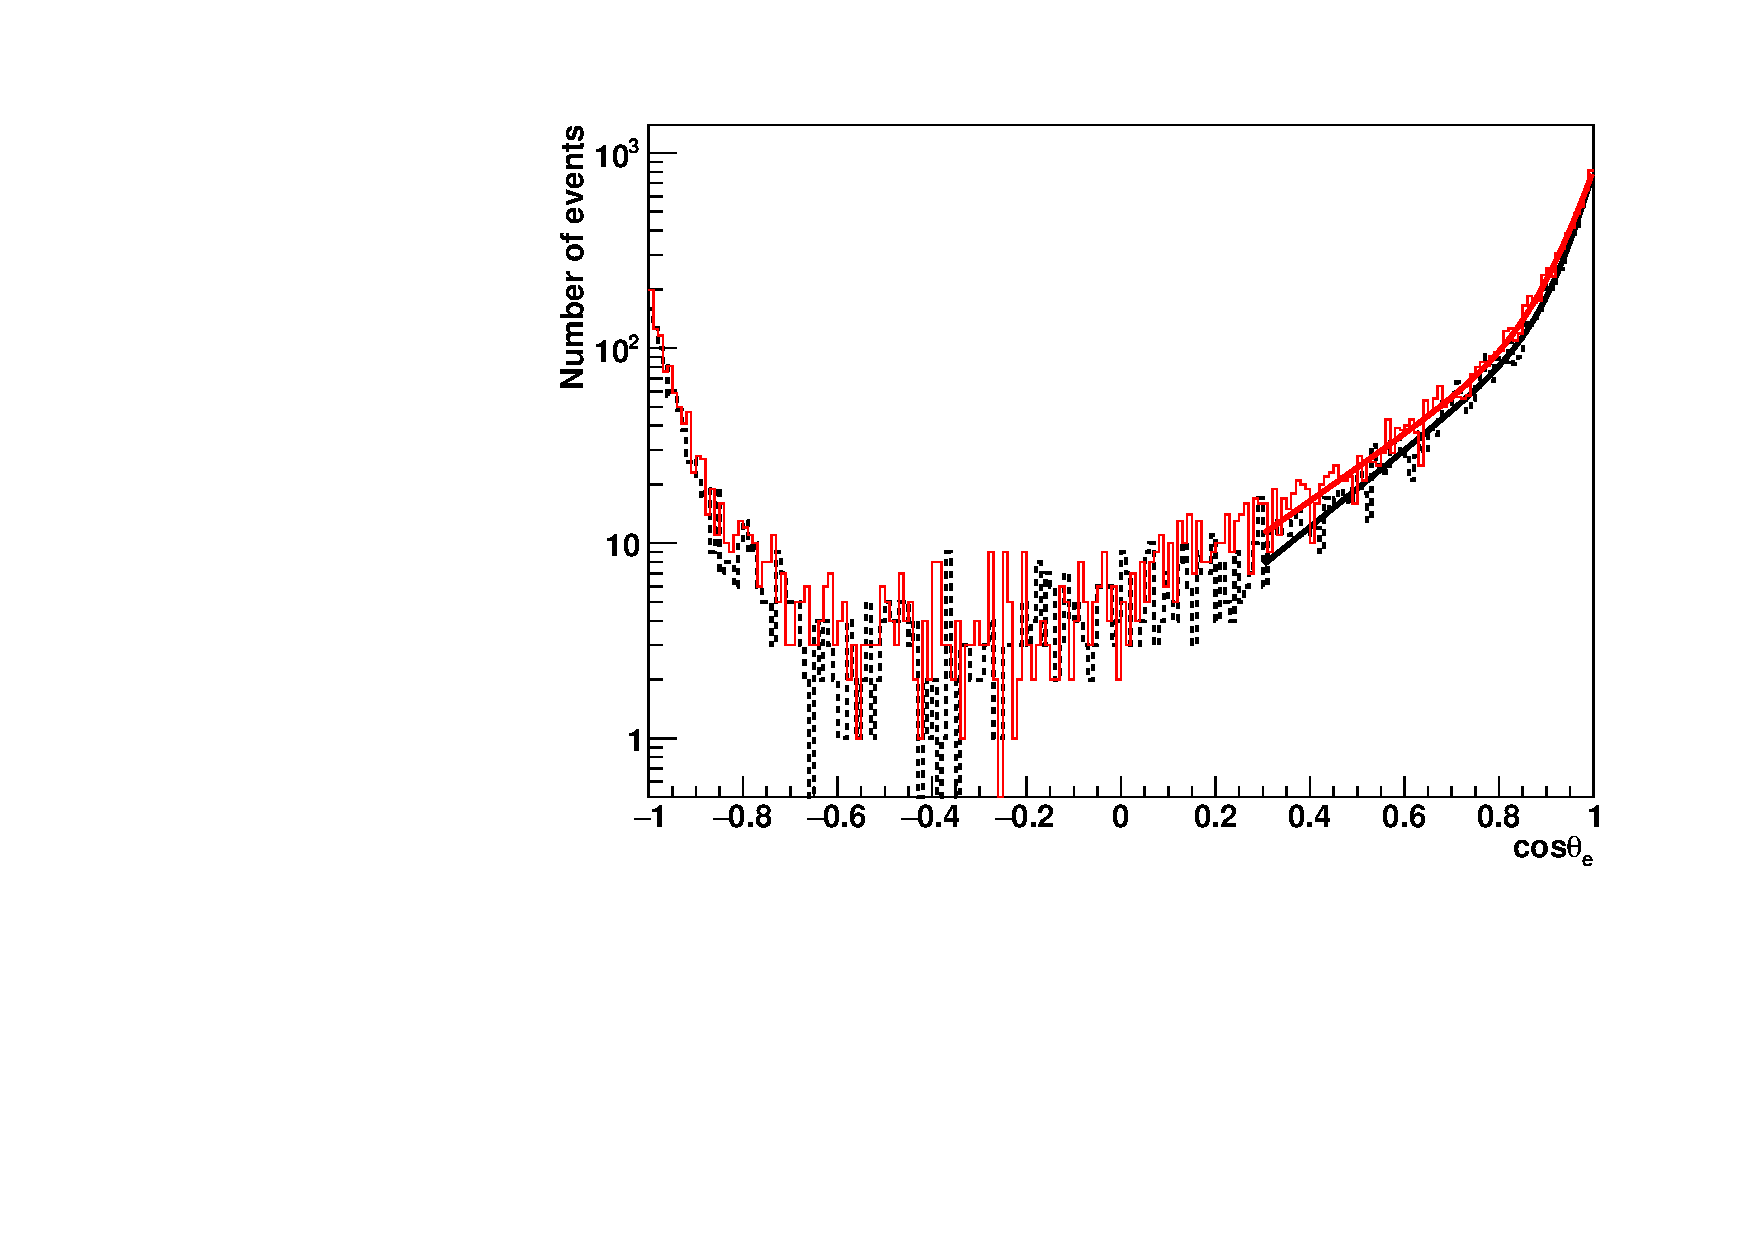
\includegraphics[width=10cm]{16NangularResol.pdf}
	\caption[Angular distributions extracted from the data and MC.]{Angular distributions extracted from the data (red solid line) and MC (black dashed line); both are reconstructed by the \texttt{MPW fitter}. These distributions are fitted with the angular resolution functions ranging from 0.3 to 1.}
	\label{angularResolMPW}
\end{figure}

\begin{table}[ht]
	\begin{tabular}{cccccccc}%{|p{2.2cm}|p{1.8cm}|p{2cm}|p{2cm}|p{1.8cm}|p{1.1cm}|p{1.1cm}|p{1.1cm}| }
		\toprule
	107055& $\beta_M$ &  $\beta_S$ & $\alpha_M$ & $\chi^2$/ndf & $\cos\theta_{0.5}$ & $\cos\theta_{0.8}$& $\cos\theta_{0.9}$\\
	\hline
	MPW data & 4.15$\pm$0.18 & 19.08$\pm$0.94 & 0.58$\pm$0.02 & 77.1/66 & 0.964 & 0.744 & 0.410 \\
	MPW MC & 4.42$\pm$0.19 & 20.41$\pm$1.01 & 0.56$\pm$0.02 & 83.8/66 & 0.974 & 0.768 & 0.454	 \\	
\hline
	\texttt{RAT} data & 3.76$\pm$0.18 & 17.90$\pm$0.82 & 0.55$\pm$0.02 & 70.5/66 & 0.974 & 0.731 & 0.364 \\
	\texttt{RAT} MC & 4.02$\pm$0.18 & 20.89$\pm$0.92 & 0.54$\pm$0.03 & 94.9/66 & 0.979 & 0.753 & 0.409	\\
		\bottomrule
	\end{tabular}
	\label{tab:angularResolValuesUpdated}
\end{table}

The resolution parameters are shown in Table.~\ref{tab:angularResolValuesUpdated}. It shows that the direction resolutions of the MC are always better than the data due to the ideal situations in the simulations. The reconstruction performance of the \texttt{MPW fitter} and the \texttt{RAT water fitter} are similar, while the $\beta_M$ values of the \texttt{MPW} are about 10\% higher than the \texttt{RAT} in both of the data and the MC. This indicates the direction resolution of the \texttt{MPW} is slightly better than the \texttt{RAT}.

\subsubsection{Direction Systematics}
For all the internal $^{16}$N scans, the cuts mentioned in the last section were applied on both the data and simulations. Similar to the evaluation of the position uncertainties, the angular resolution function was first fitted with three free parameters: $\alpha_M$, $\beta_S$, and $\beta_M$. To simplify the calculation in propagating systematics, an average value of the fitted $\alpha_M$ was calculated from all the internal scans (except the three neck scans), as 0.613 for data and 0.585 for MC. With the fixed values of $\alpha_M$, both the data and the MC were refit with $\beta_S$ and $\beta_M$ only. The default fit range is [0.3,1], while for some scans close to the AV, the events can be few after the cuts. For these situations, to ensure more than 5000 events were fitted, the fit range was enlarged by moving a 0.1 step to the left until the left value reaches -0.5: $[0.3-0.1\cdot step,1]$.

Fig.~\ref{angularResolScan} shows the results of the fitted $\beta_M$ and $\beta_S$ values for the internal $^{16}$N x, y and z-axes scans. It shows that for most of the scans, the MC results are better than the data. The three Z scans in the neck have the worst direction resolutions due to the asymmetry of the detector geometry. 

\begin{figure}
	\centering
	\subfigure[$^{16}$N x-scan runs.]{\label{angular:xscan}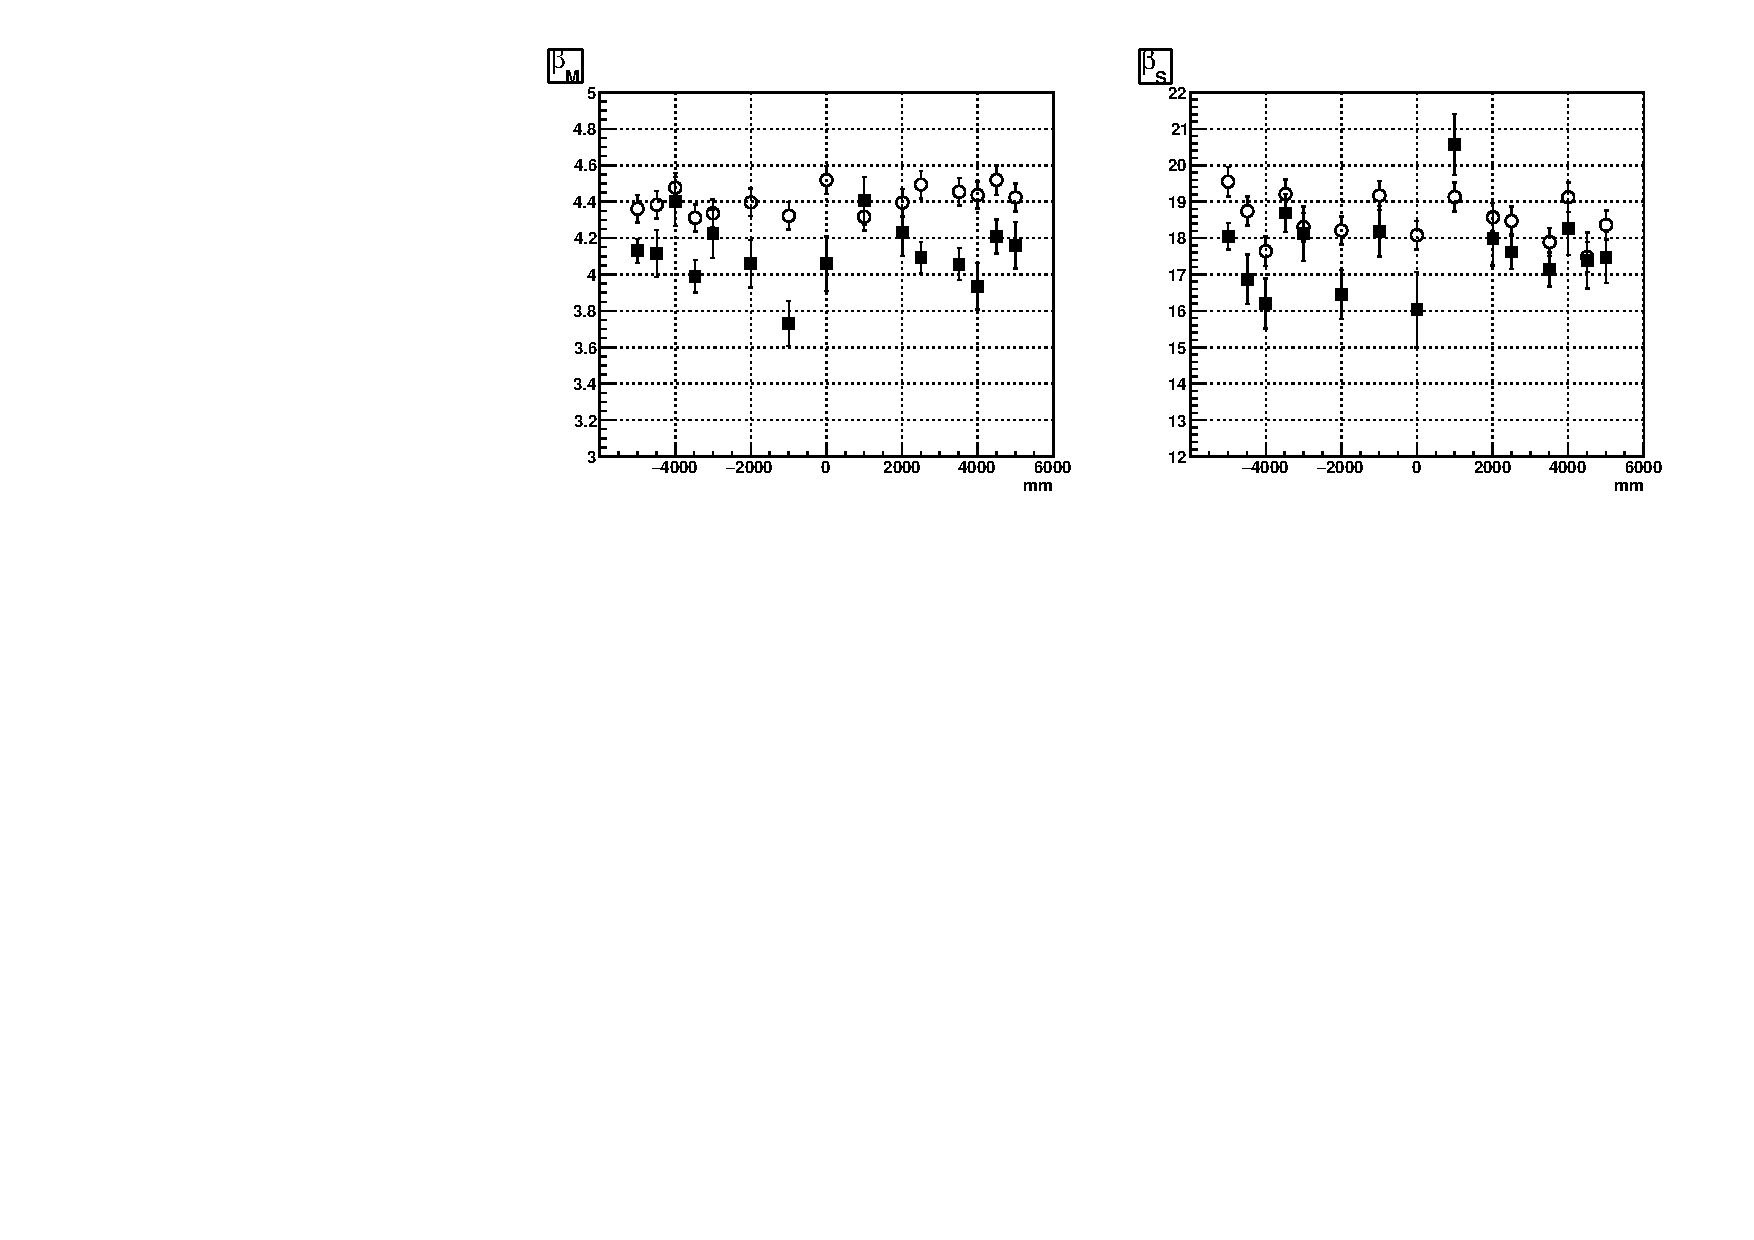
\includegraphics[width=12cm]{16NangularScan_x.pdf}}
	\subfigure[$^{16}$N y-scan runs.]{\label{angular:yscan}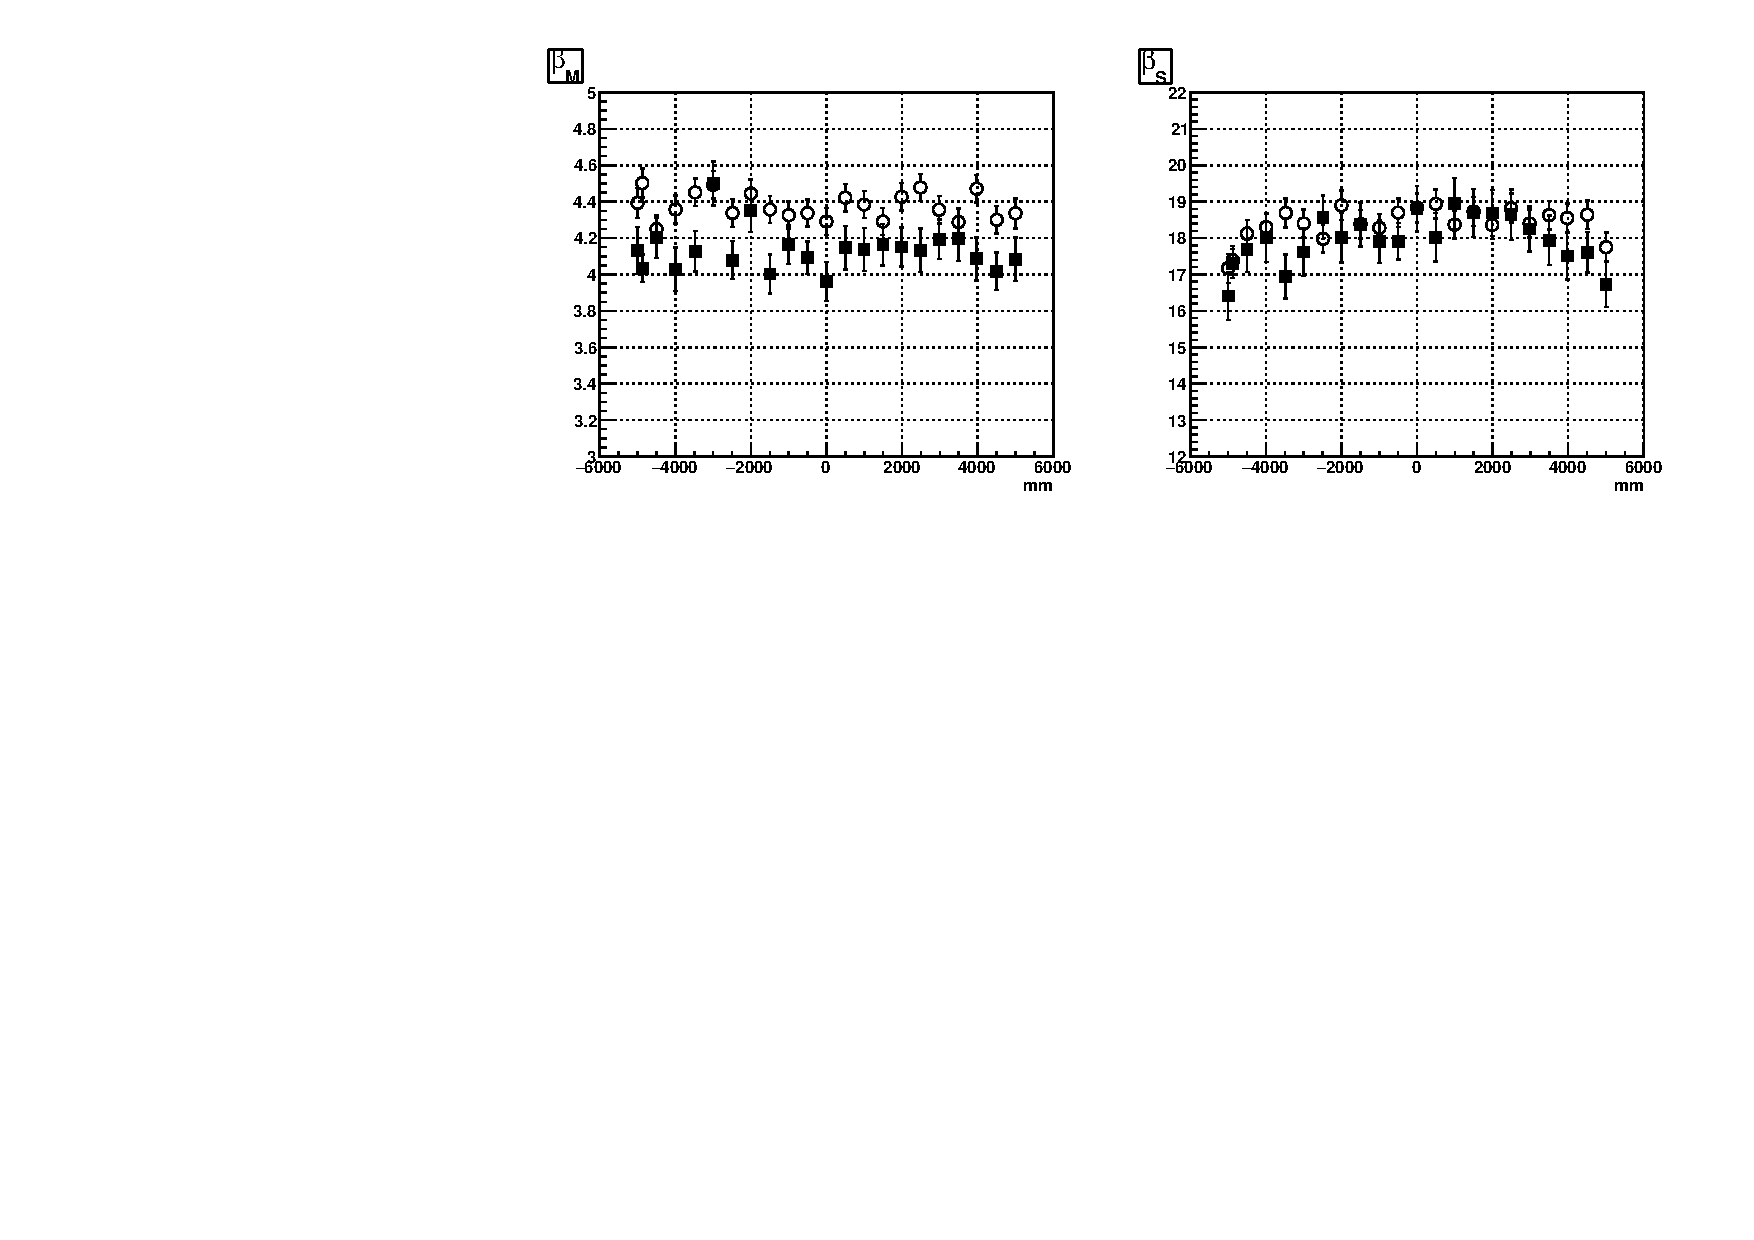
\includegraphics[width=12cm]{16NangularScan_y.pdf}}
	\subfigure[$^{16}$N z-scan runs.]{\label{angular:zscan}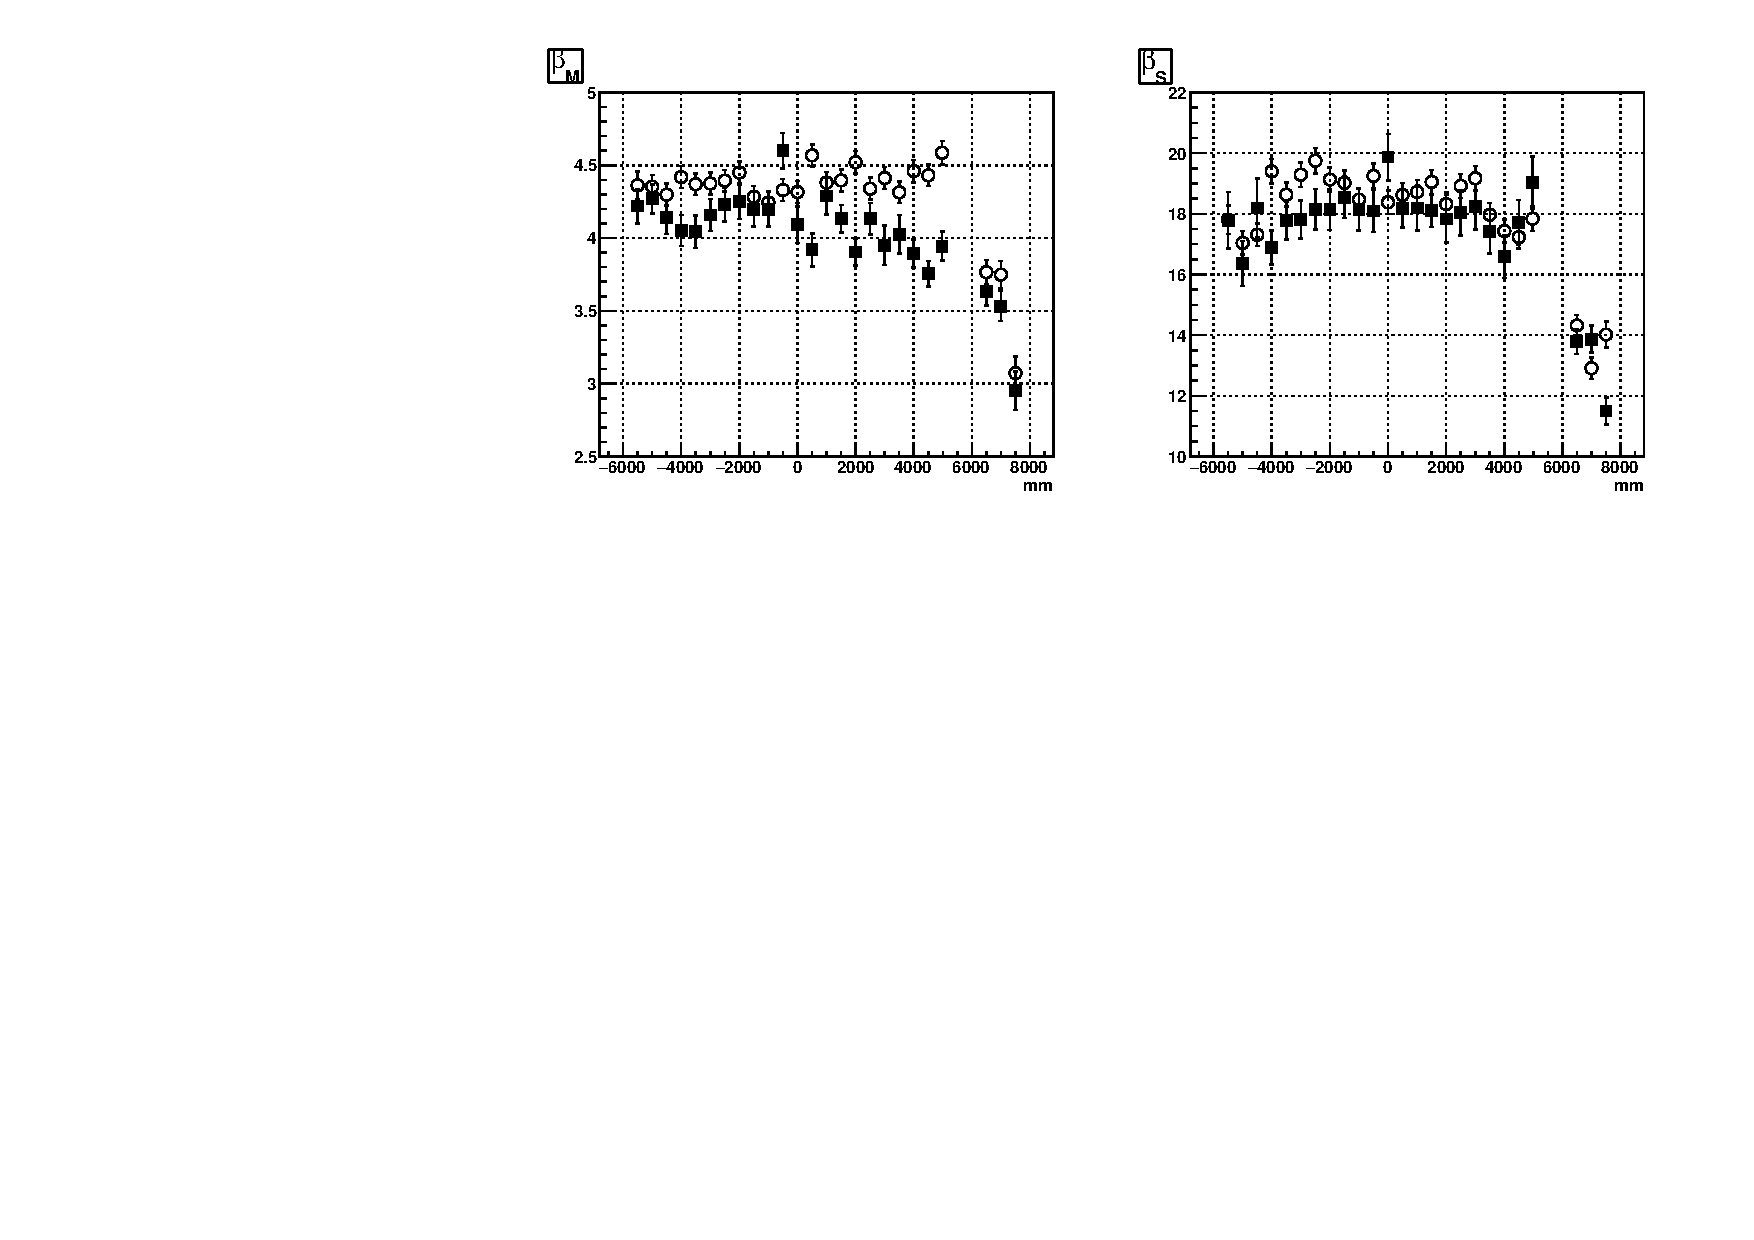
\includegraphics[width=12cm]{16NangularScan_z.pdf}}
	\caption{Fitted direction resolution parameters $\beta_M$, $\beta_S$ for the source scans in x, y, z-axes respectively.}
	\label{angularResolScan}
\end{figure}

The relative difference between data and MC of a fitted resolution quantity $q\pm \delta_q$ is defined as:
\begin{equation}
(\Delta q)_{rel} = \frac{q_{data}-q_{MC}}{q_{MC}}\times 100\%.
\end{equation}

The error of the relative difference is defined as: 
\begin{equation}
\delta_{(\Delta q)_{rel}} = \sqrt{(\frac{\delta_{q_{data}}}{q_{data}})^2+(\frac{\delta_{q_{MC}}}{q_{MC}})^2}\times 100\%.
\end{equation}\label{eq:erors_relativeBiases}

Fig.~\ref{relative_biasesVsPositions} shows the relative differences for the internal x, y, z scans (not using the neck scans).
\begin{figure}[!htb]
	\centering
	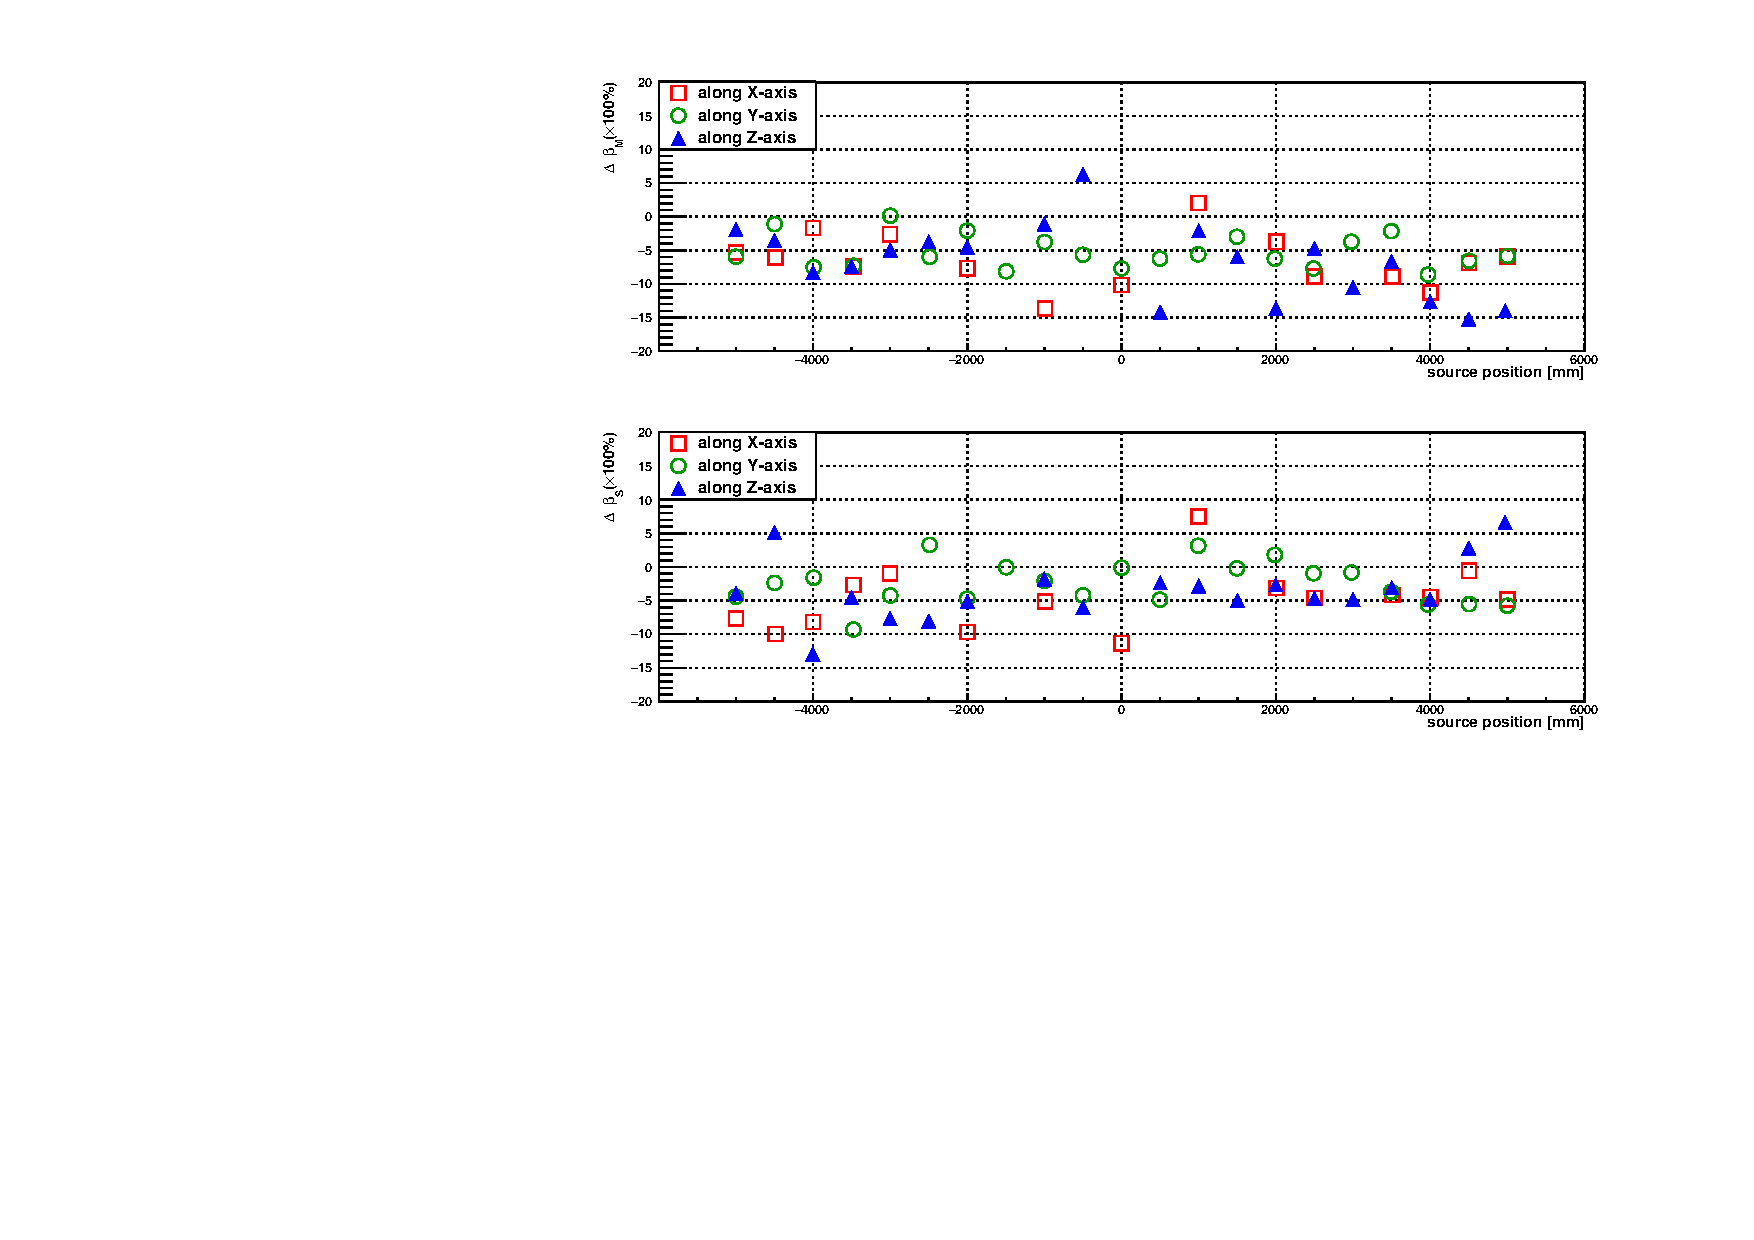
\includegraphics[width=16cm]{angularResol_scanXYZ.pdf}
	\caption[Relative differences of $\beta_M$ and $\beta_S$ as a function of the $^{16}$N source position.]{Relative differences of $\beta_M$ and $\beta_S$ as a function of the $^{16}$N source position. For simplicity, the corner scans are not shown in this figure. The red squares represent the results from the x-scan runs; green circles represent the y-scan runs and the blue triangles represent the z-scan runs.}
	\label{relative_biasesVsPositions}
\end{figure}

Taking the internal scans except the neck scans (77 runs in total), the means and standard deviations of the relative differences are:

$\Delta(\beta_M)_{rel}=(-6.09\pm4.01)\%$, and $\Delta(\beta_S)_{rel}=(-3.09\pm4.39)\%$.

To be conservative, taking the largest and smallest values of the $\Delta(\beta_M)_{rel}$ and $\Delta(\beta_S)_{rel}$, the negative and positive values of the direction systematic ($\delta_\theta$) are obtained as $\delta_\theta=+0.013/-0.101$.

To propagate the uncertainties of $\beta$ to the direction resolution, a first-order approximation function was derived by the SNO collaboration\cite{drouin2012three}:
\begin{equation}\label{remapTheta}
\cos\theta'=1+(\cos\theta-1)(1+\delta_{\theta}).
\end{equation} 

This angular remapping function is used to smear the angular distributions for systematic studies. In the next chapter, it will be applied on the angular distribution of solar neutrino data. 

\subsection{$\beta_{14}$ and Its Systematic}
Since $\beta_{14}$ itself is used as the high-level cut, only the cuts of $ITR>0.55$ and NHits$>5$ were applied on the data and MC to extract the $\beta_{14}$ distributions.
Fig.~\ref{fig:N16beta14} shows the $\beta_{14}$ distributions of the central run-107055 data and MC, reconstructed by the \texttt{MPW fitter} and the official \texttt{RAT} fitter respectively. The $\beta_{14}$ is calculated based on the reconstructed position, time, and direction of an event while the $\beta_{14}$ distributions from the \texttt{MPW} and the \texttt{RAT} results are consistent. However, both of the two fitters show a discrepancy between the data and the MC. This discrepancy can be caused by inaccurate modeling of the Cherenkov process in the Geant4 simulation\cite{dunmore2004separation,beta14discrepancy}.
Fig.~\ref{fig:N16beta14MPW} shows a comparison of the $\beta_{14}$ for the data and the MC in run-107055. Both of the distributions are the MPW processed results and are fitted with Gaussian distributions in a region of $[-0.5,1.5]$. The data shows a smaller Gaussian mean value, $\mu_{data}=0.4157$, compared to the $\mu_{MC}=0.4388$.

\begin{figure}[htbp]
	\centering
	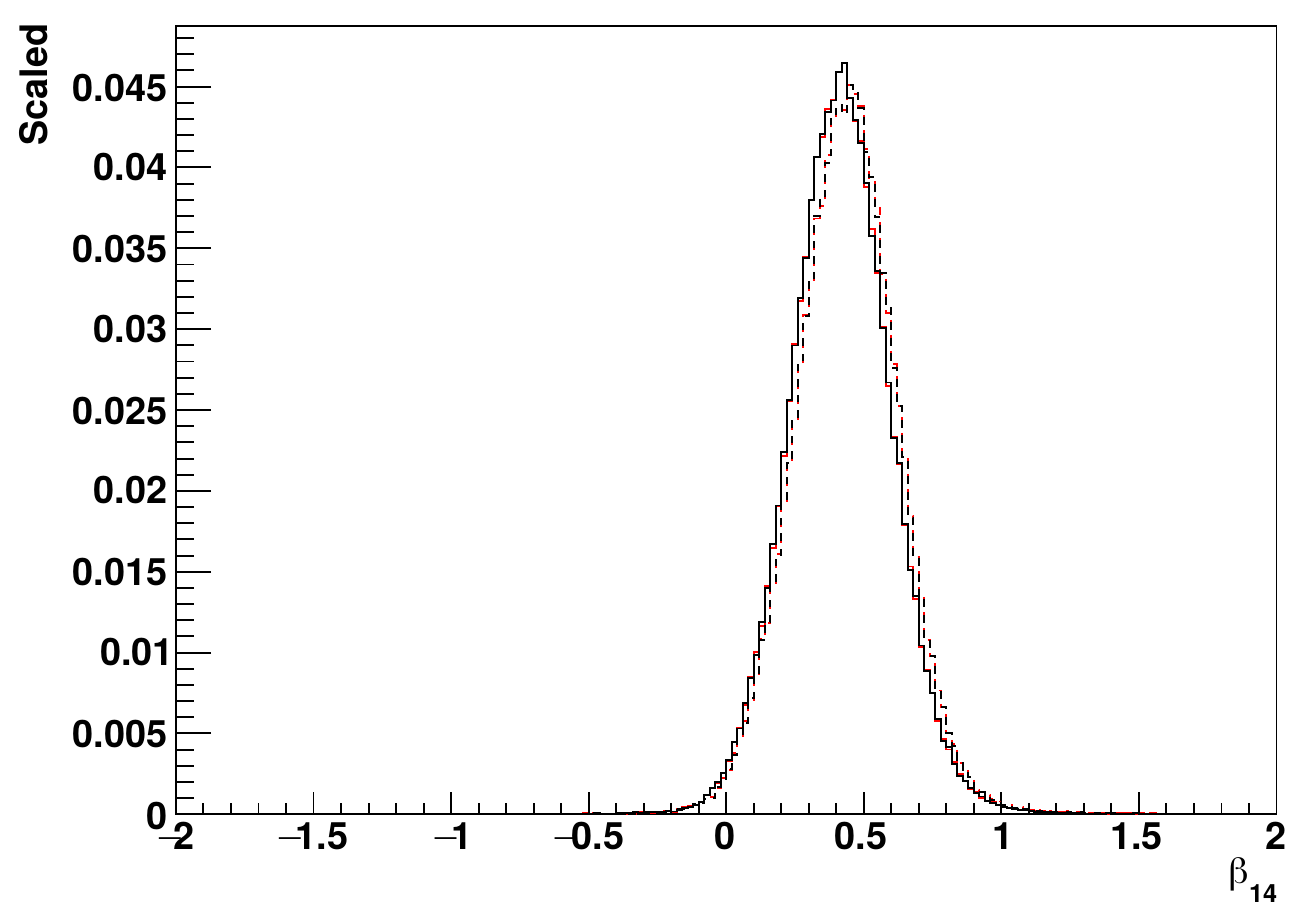
\includegraphics[width=8cm]{N16_beta14_107055.png}
	\caption[Distributions of $\beta_{14}$ for the $^{16}$N central run-107055.]{Distributions of $\beta_{14}$ for the $^{16}$N central run-107055. Dashed lines for the MC and solid lines for data; red for the \texttt{MPW fitter} processed results and black for the \texttt{RAT} results.}
	\label{fig:N16beta14}
\end{figure}

\begin{figure}[htbp]
	\centering
	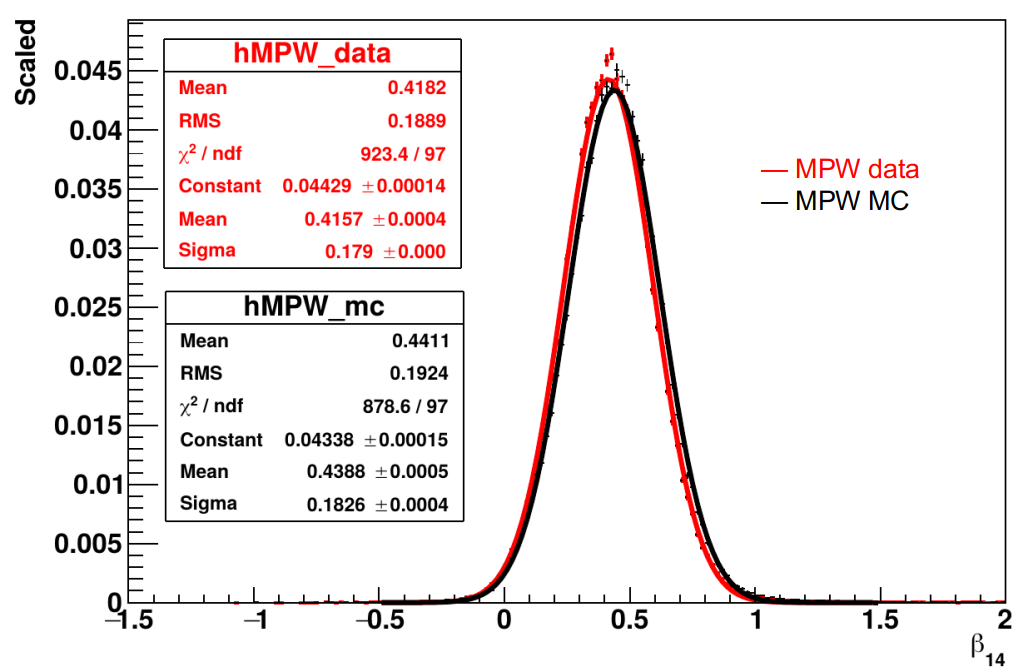
\includegraphics[width=8cm]{N16FitMPW_beta14_107055.png}
	\caption{A comparison of the $\beta_{14}$ for the data and the MC in run-107055.}
	\label{fig:N16beta14MPW}
\end{figure}

Fig.~\ref{beta14_XYZscans} shows effects when the source moving along x, y and z axes. Taking all the 80 internal runs mentioned before, I calculated the $\Delta \beta_{14}\equiv\mu_{data}-\mu_{MC}$ for each run. The mean and standard deviation of these $\Delta \beta_{14}$ values were taken as the shift in $\beta_{14}$: $-0.026\pm0.010$. Following the suggestion in Ref.~\cite{waterunidoc}, an asymmetric uncertain was taken: the upward shift was taken as $+0.010$ while the downward was taken as $-0.026-0.01=-0.036$. Thus the shifts: $+0.010/-0.036$ was taken as the $\beta_{14}$ systematics. It will be applied to the solar neutrino analysis in the next chapter. 

\begin{figure}[htbp]
	\centering
	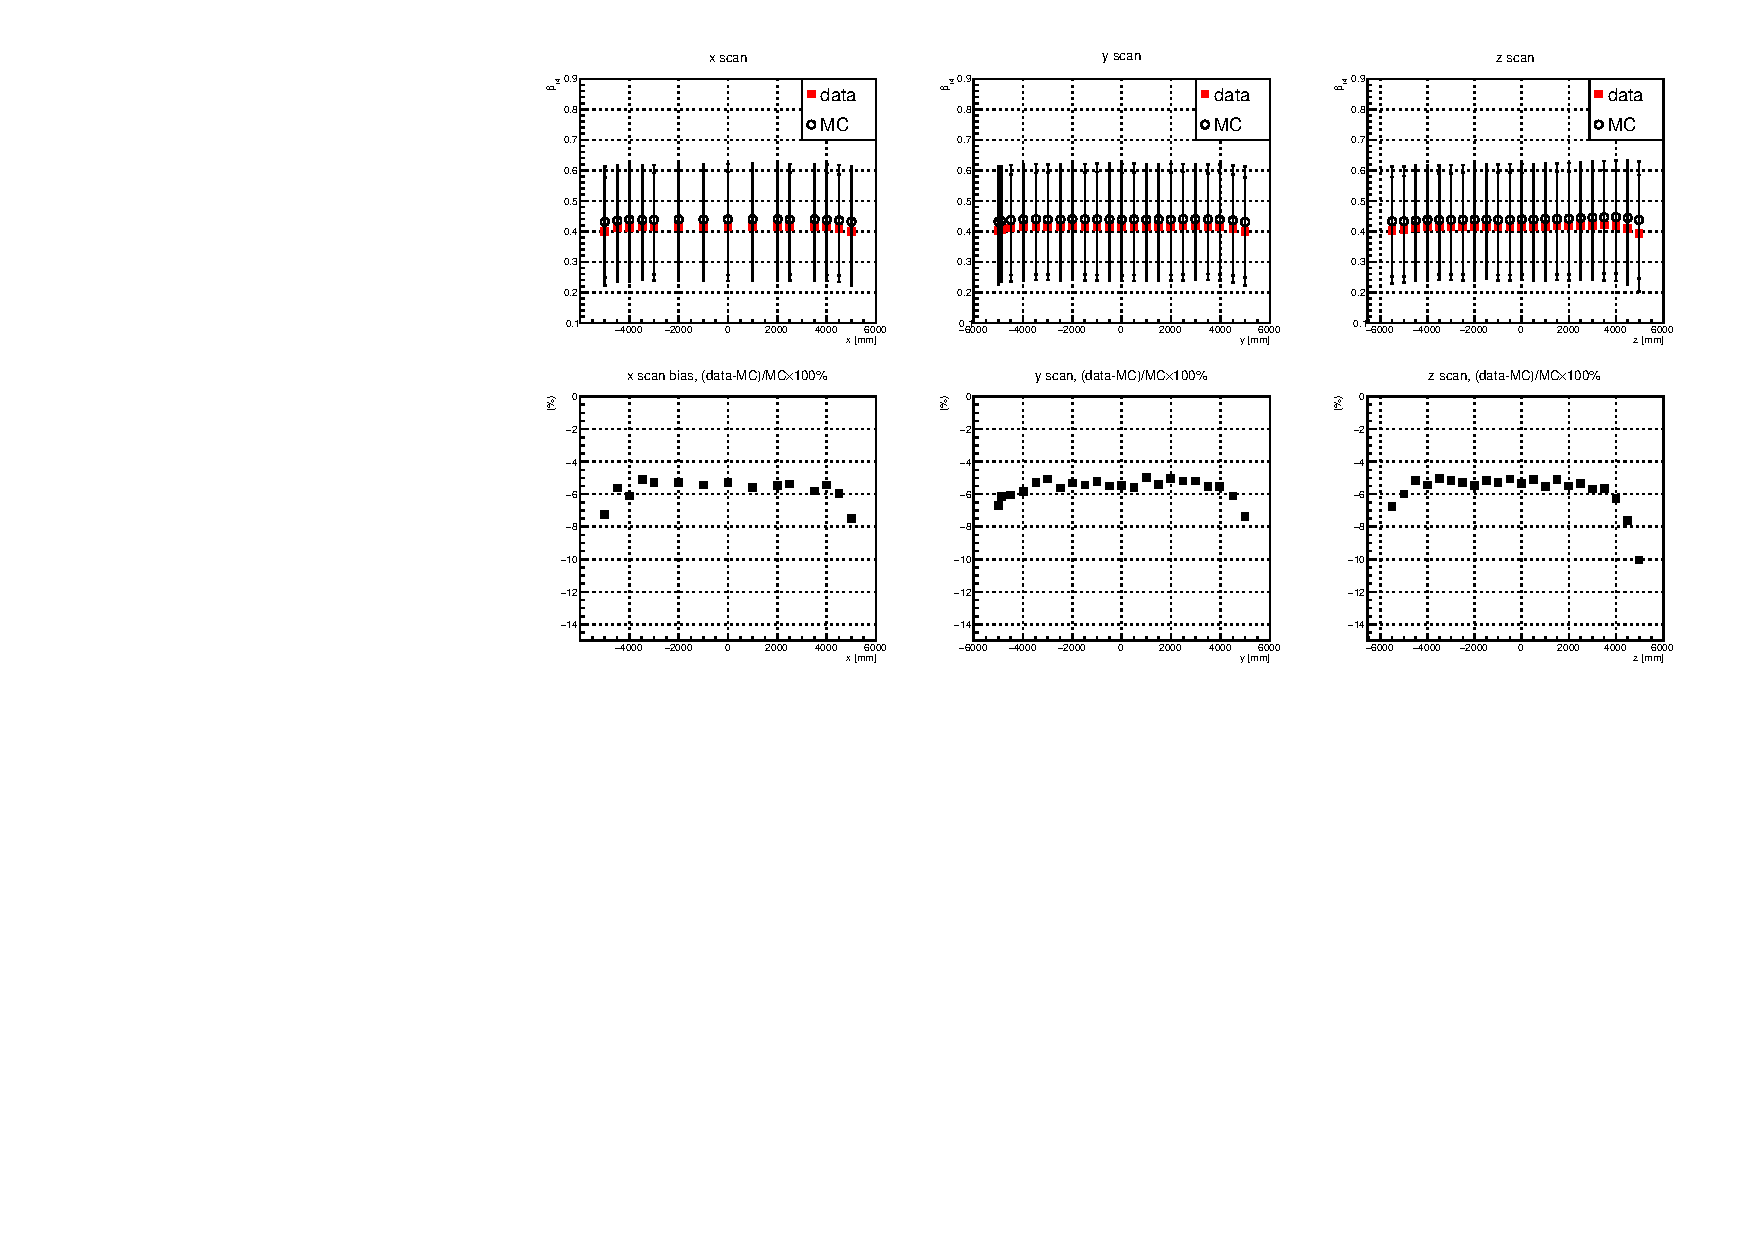
\includegraphics[width=15cm]{beta14_xyzScans.pdf}
	\caption{$\beta_{14}$ systematic along x, y, z scans.}
	\label{beta14_XYZscans}
\end{figure}
%Discussions for the external scan runs.
%For external scans, the radial cuts were not applied. 

%\begin{figure}[!htb]
%	\centering
%	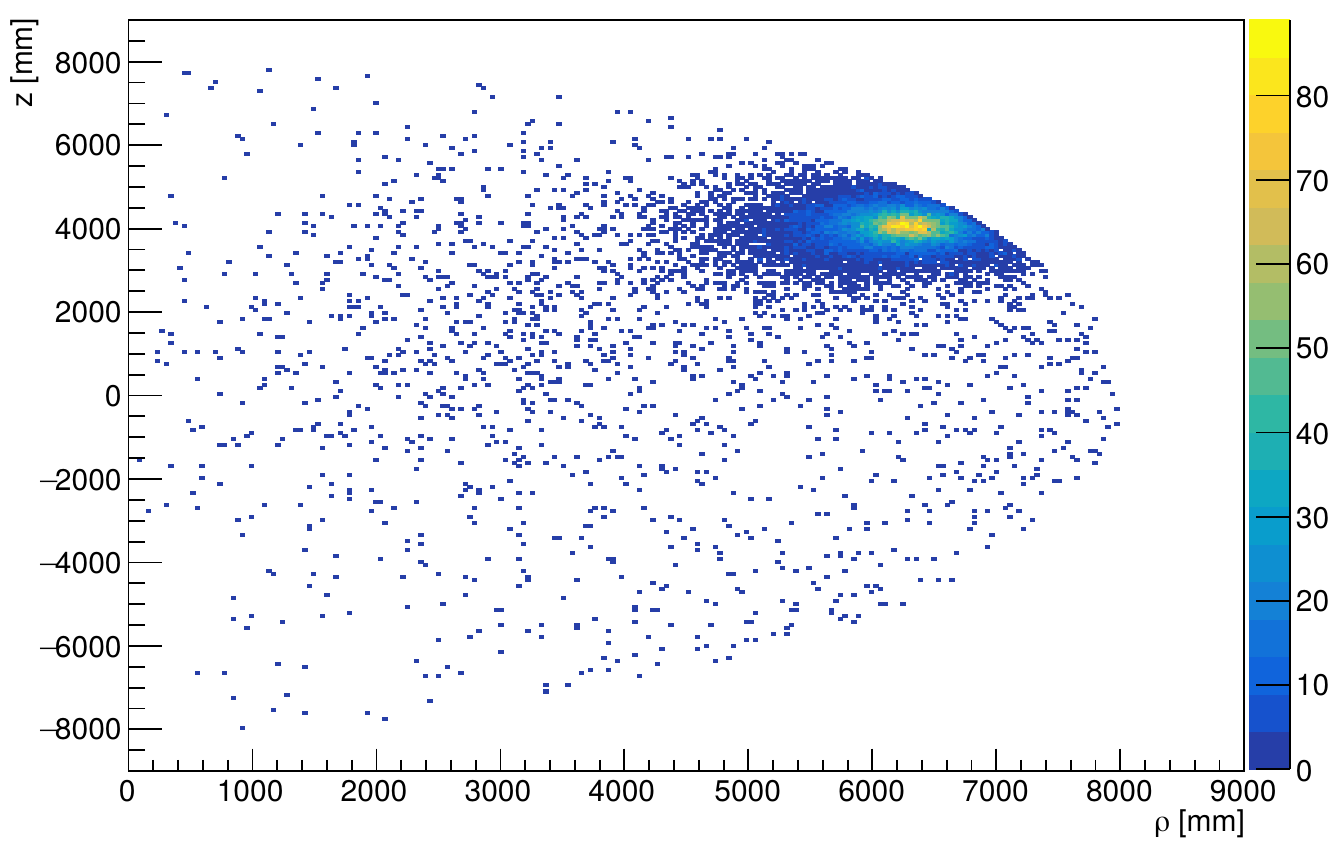
\includegraphics[width=8cm]{N16_external_111230_rhoZ.png}
%	\caption{$^{16}$N external run-111230 with a nominal position at [-5861,-2524,4001] mm; MPW results.}
%	\label{16Nexternal}
%\end{figure}

\subsection{Energy Reconstruction Evaluation}
\subsubsection{Energy Figure of Merits}\label{sect:energy_fomTest}
Three energy FoM quantities: $G_{test}$, $U_{test}$ and $Z_{factor}$ were introduced in Sect.~\ref{sect:energy_fom}.
Here I used the MC simulations as well as the data of the $^{16}$N central run-107055 to check the effects of the cuts on FoM quantities to reduce the energy biases. The sacrifices of the events were calculated. 

%Then the data of the same run were used to check the ratios off by the FOM quantities. 

\begin{itemize}
	\item[$\bullet$]$U_{test}$:
	Fig.~\ref{energyFOM_Utest} shows $U_{test}$ vs. energy biases. A cut of $0.61<U_{test}<0.95$ was suggested by the collaboration, to remove the events were mostly caused by the source encapsulation. This cut removes 0.38\% of MC events and 0.34\% of data events.
	\begin{figure}[!htb]
		\centering
		%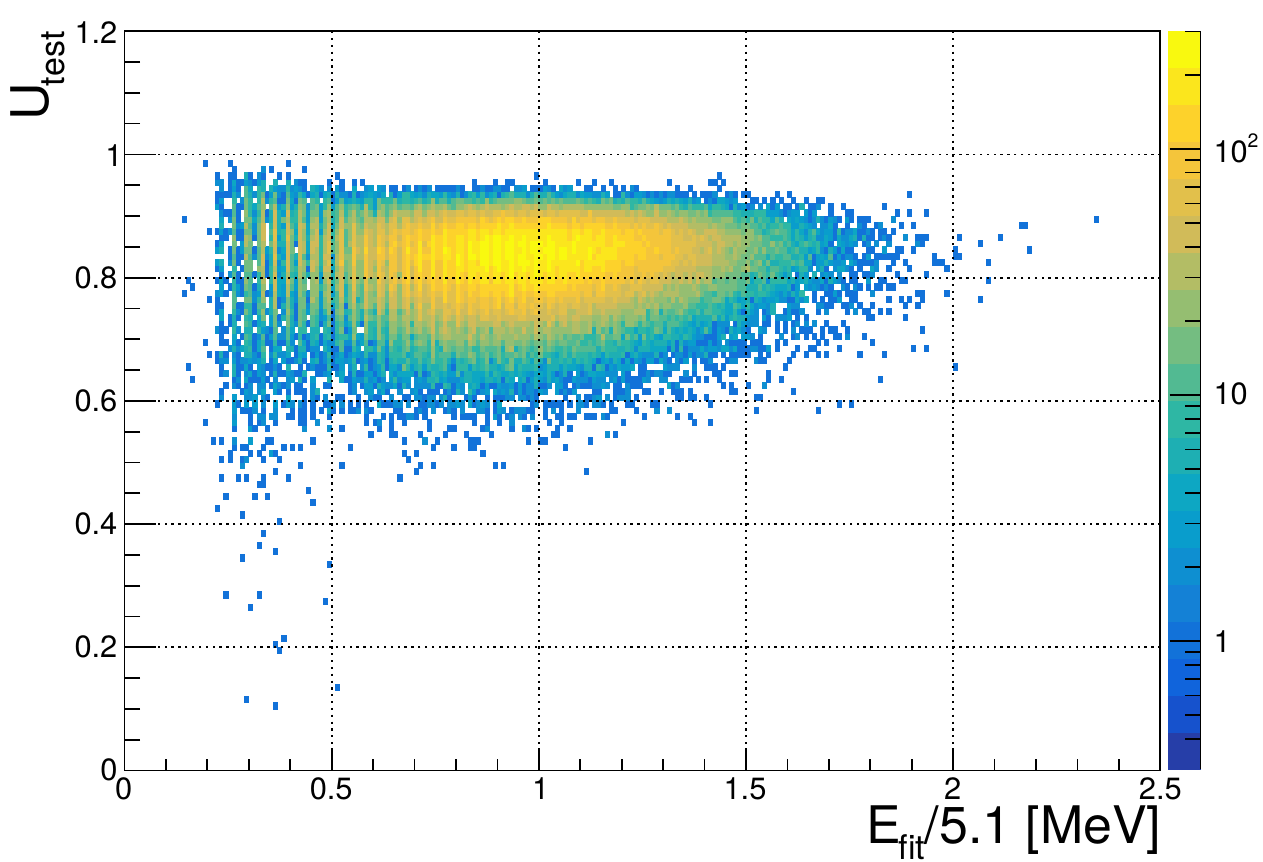
\includegraphics[width=8cm]{Utest_data_N16_107055.png}
		\subfigure[MC]{ 
			\begin{minipage}[t]{0.5\textwidth}
				\centering
				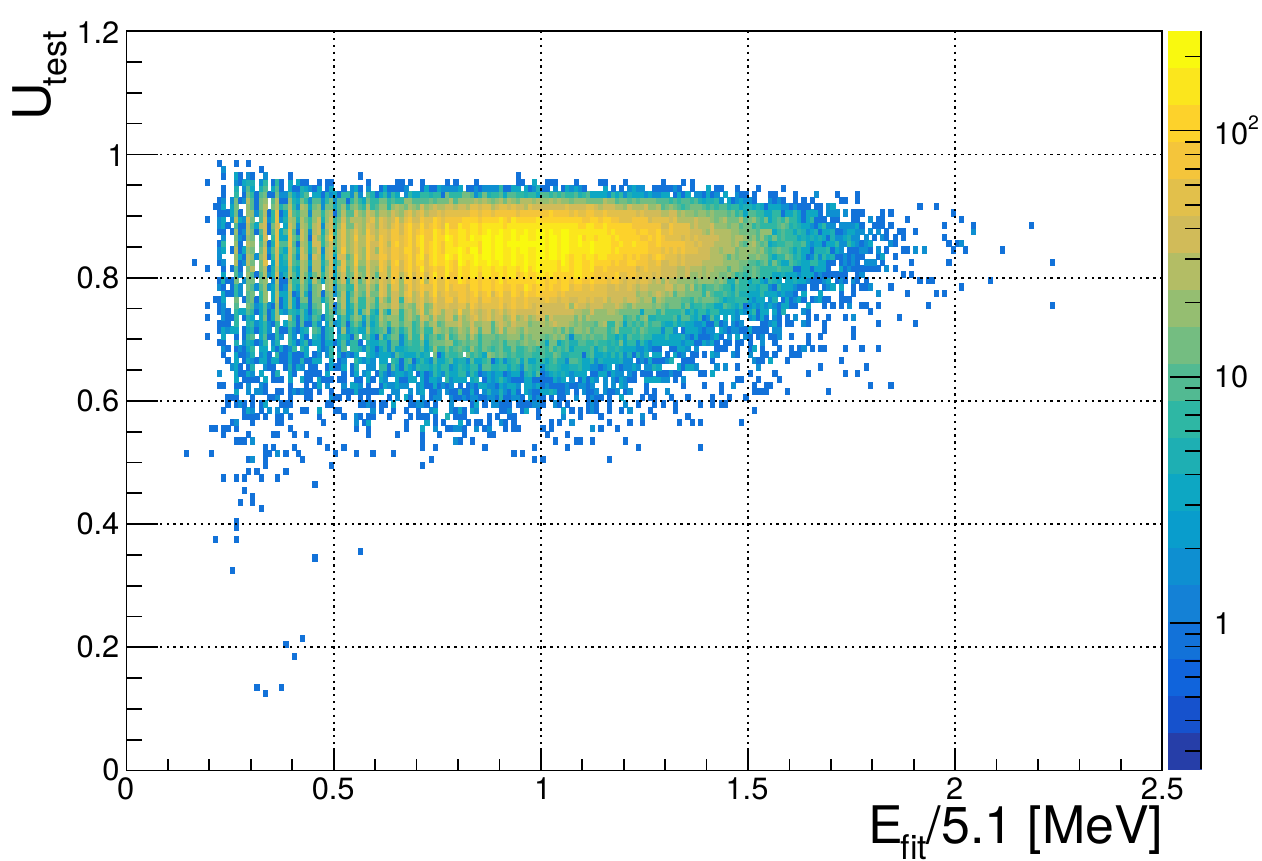
\includegraphics[width=7.5cm]{Utest_MC_N16_107055.png}
			\end{minipage}
		}
		\subfigure[data]{ 
			\begin{minipage}[t]{0.4\textwidth}
				\centering
				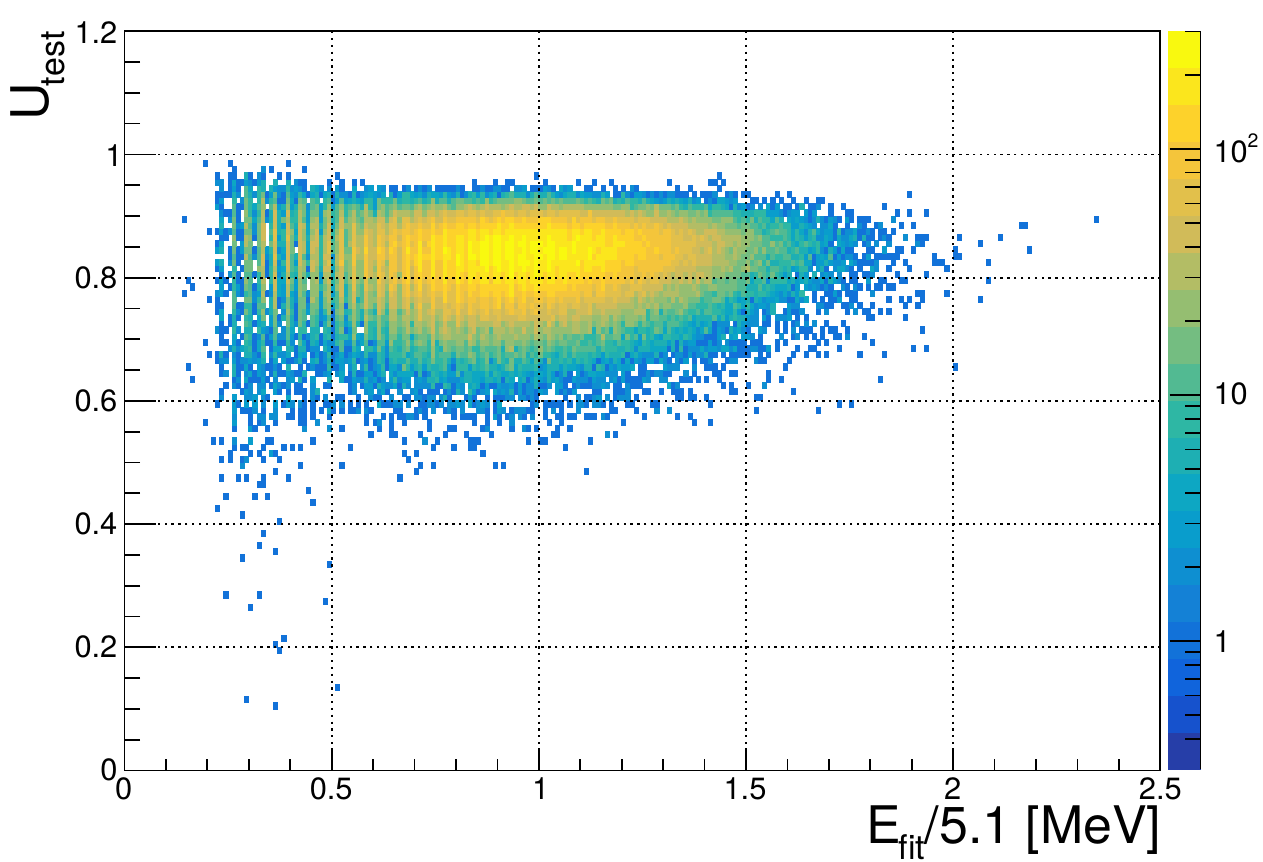
\includegraphics[width=7.5cm]{Utest_data_N16_107055.png}
			\end{minipage}
		}
		\caption{$^{16}$N central-run 107055, $U_{test}$ vs. $E_{fit}$/5.1 MeV.}
		\label{energyFOM_Utest}
	\end{figure}
	
	\item[$\bullet$] $G_{test}$: Fig.~\ref{energyFOM_Gtest} shows $G_{test}$ vs. energy biases. A cut of $0<G_{test}<1.9$ was suggested by the collaboration, which removes 0.01\% events for both MC and data.	
	
	\begin{figure}[!htb]
		\centering
		\subfigure[MC]{ 
			\begin{minipage}[t]{0.5\textwidth}
				\centering
				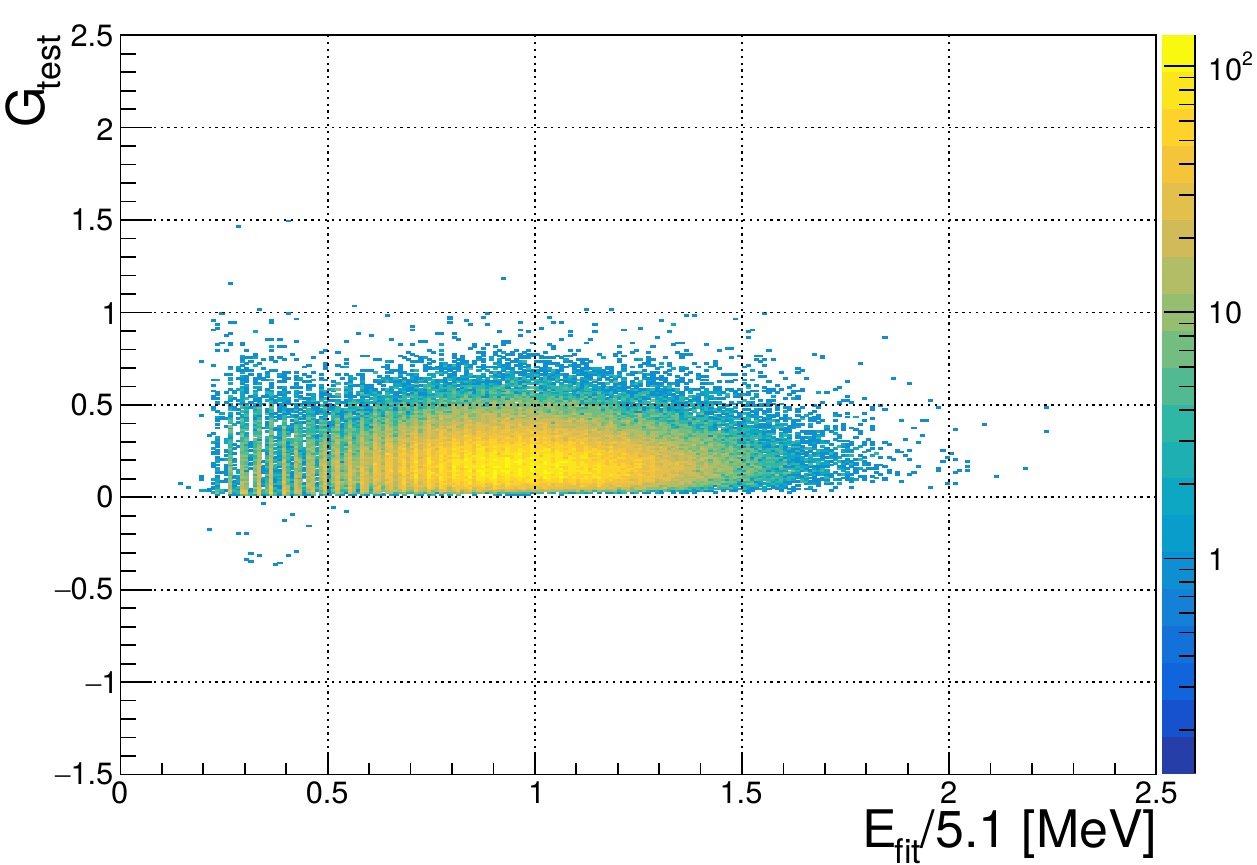
\includegraphics[width=7.5cm]{Gtest_MC_N16_107055.png}
			\end{minipage}
		}
		\subfigure[data]{ 
			\begin{minipage}[t]{0.4\textwidth}
				\centering
				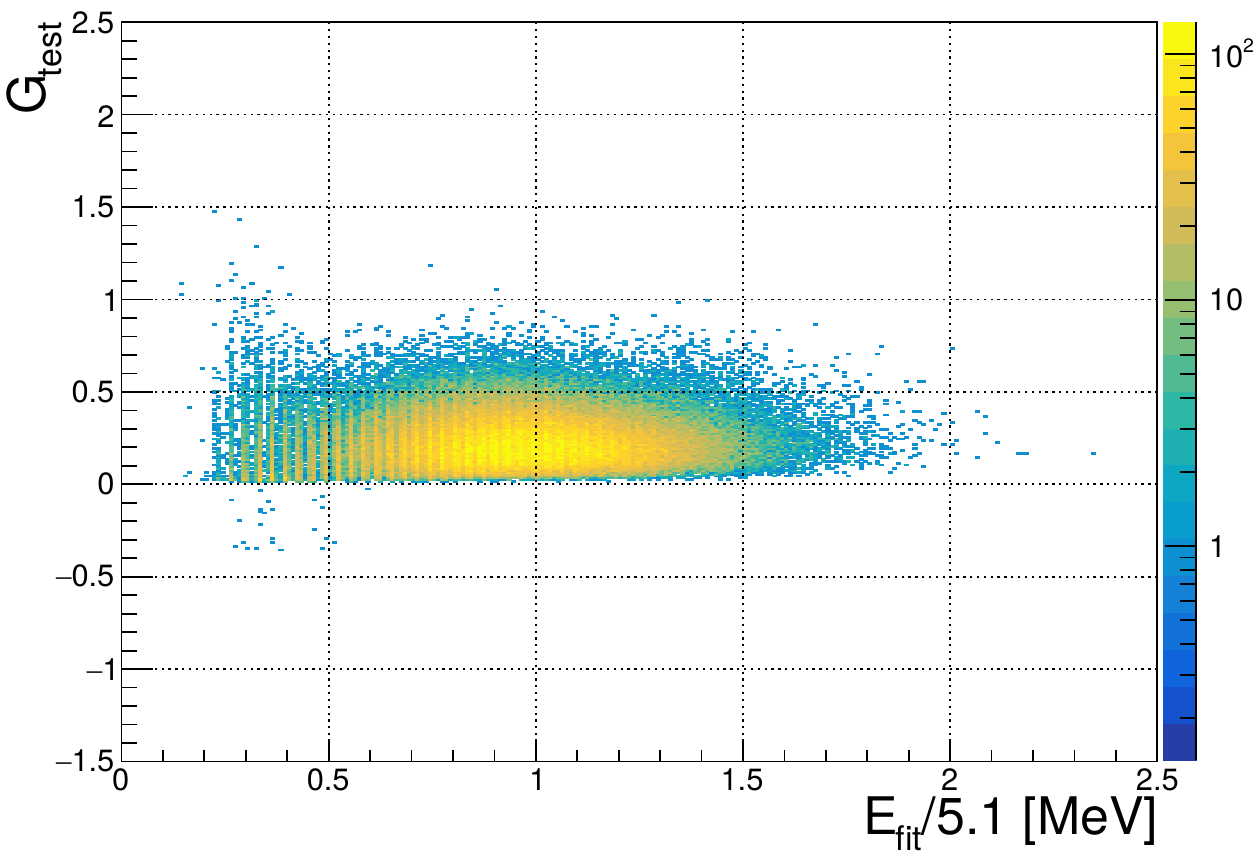
\includegraphics[width=7.5cm]{Gtest_data_N16_107055.png}
			\end{minipage}
		}
		\caption{$^{16}$N central-run 107055, $G_{test}$ vs. $E_{fit}$/5.1 MeV.}
		\label{energyFOM_Gtest}
	\end{figure}
	
	\item[$\bullet$]$Z_{factor}$:
	Fig.~\ref{energyFOM_Zfactor} shows $Z_{factor}$ vs. energy biases. A cut of $-11<Z_{factor}<1$ was suggested by the collaboration, which removes 0.13\% events for both MC and data.		
	\begin{figure}[!htb]
		\centering
		\subfigure[MC]{ 
			\begin{minipage}[t]{0.5\textwidth}
				\centering
				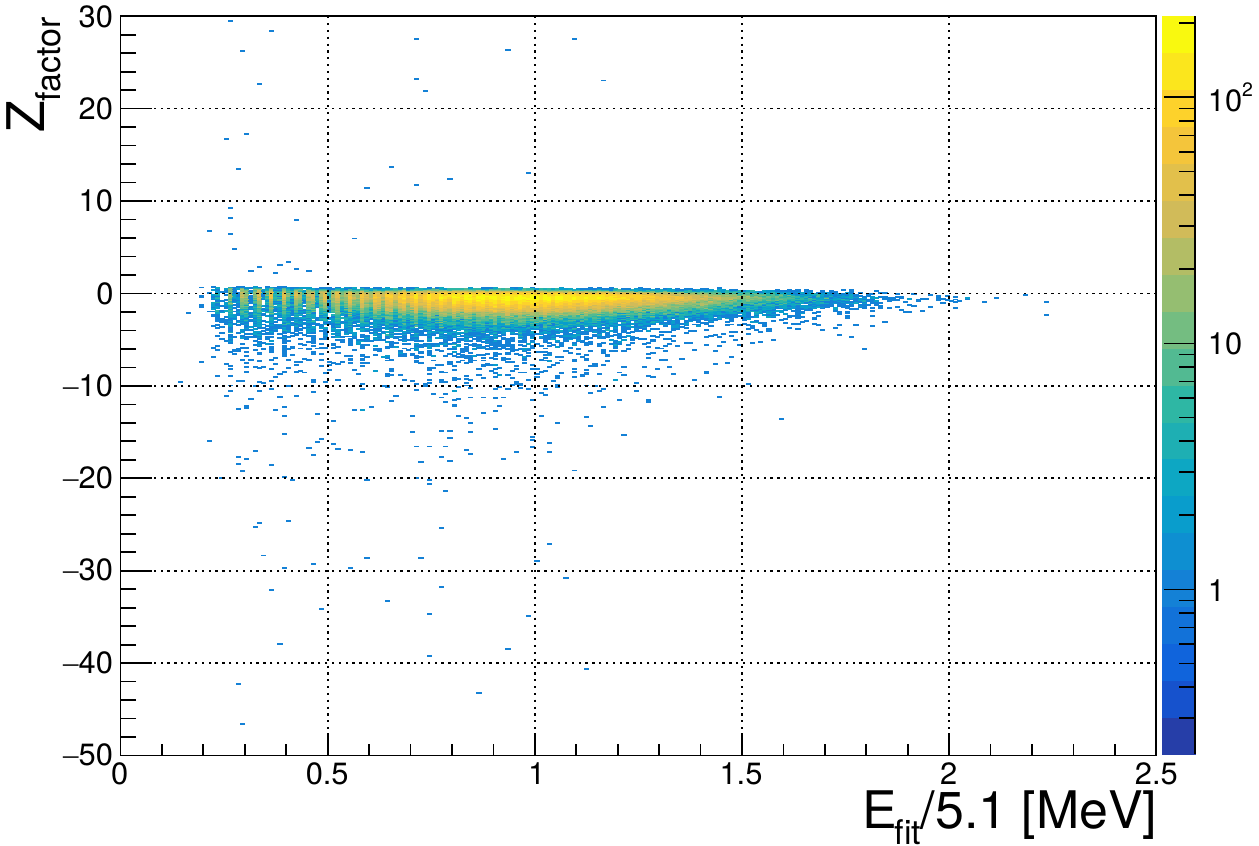
\includegraphics[width=7.5cm]{Zfactor_MC_N16_107055.png}
			\end{minipage}
		}
		\subfigure[data]{ 
			\begin{minipage}[t]{0.4\textwidth}
				\centering
				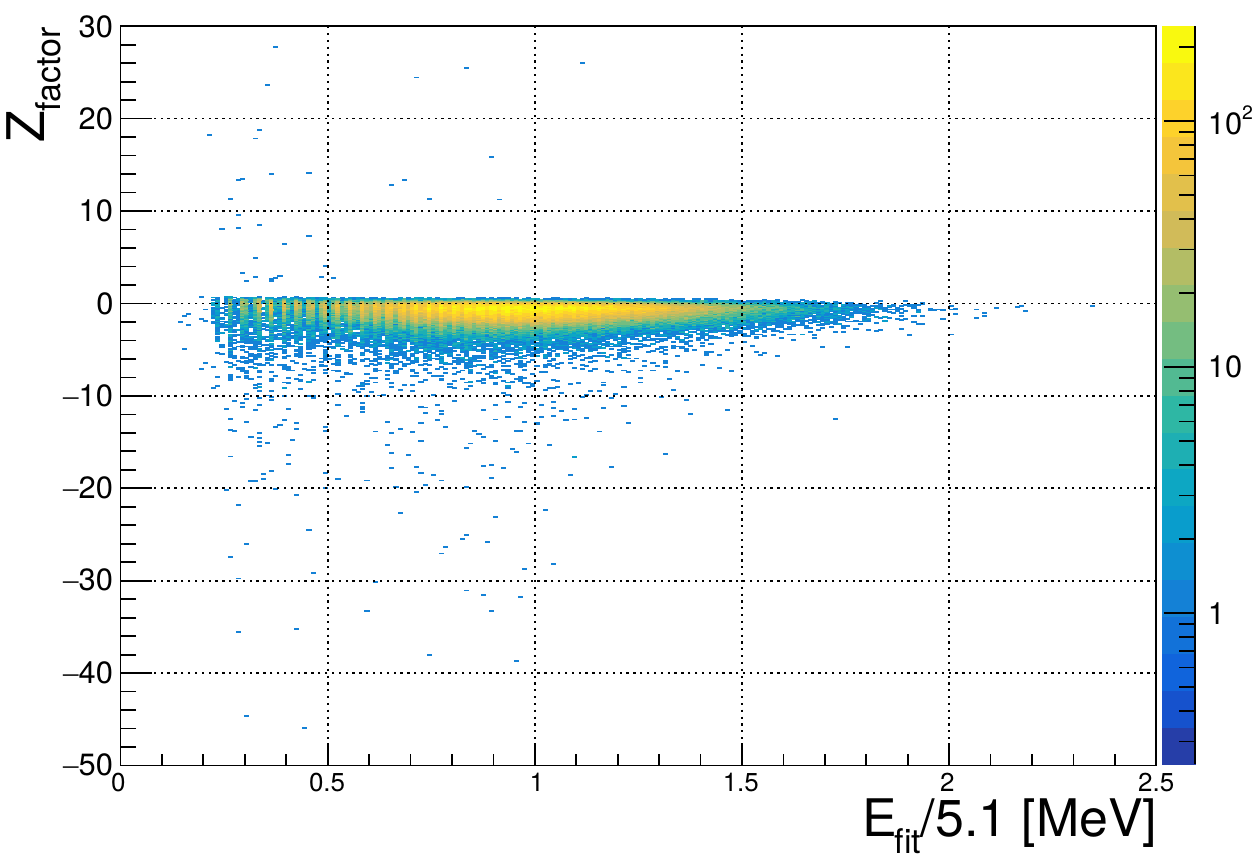
\includegraphics[width=7.5cm]{Zfactor_data_N16_107055.png}
			\end{minipage}
		}
		\caption{$^{16}$N central-run 107055, $Z_{factor}$ vs. $E_{fit}$/5.1 MeV.}
		\label{energyFOM_Zfactor}
	\end{figure}
	
	
\end{itemize}

All the cuts on the three energy FoM quantities remove 0.40\% events from MC and 0.37\% events from data. These cuts were also used in the water phase analysis in Chapter 6.

\subsubsection{Energy Resolution and Systematics}
The energy reconstruction algorithms for the water phase (mentioned in Sect.~\ref{sect:energyFitter}, Chapter 4) was applied on the $^{16}$N MC simulations and data. The reconstructed energy of the $^{16}$N events are shown in Fig.~\ref{fig:N16energy}. The results from the MC and the data are compared.

\begin{figure}[htbp]
	\centering
	\subfigure[$^{16}$N run-106925]{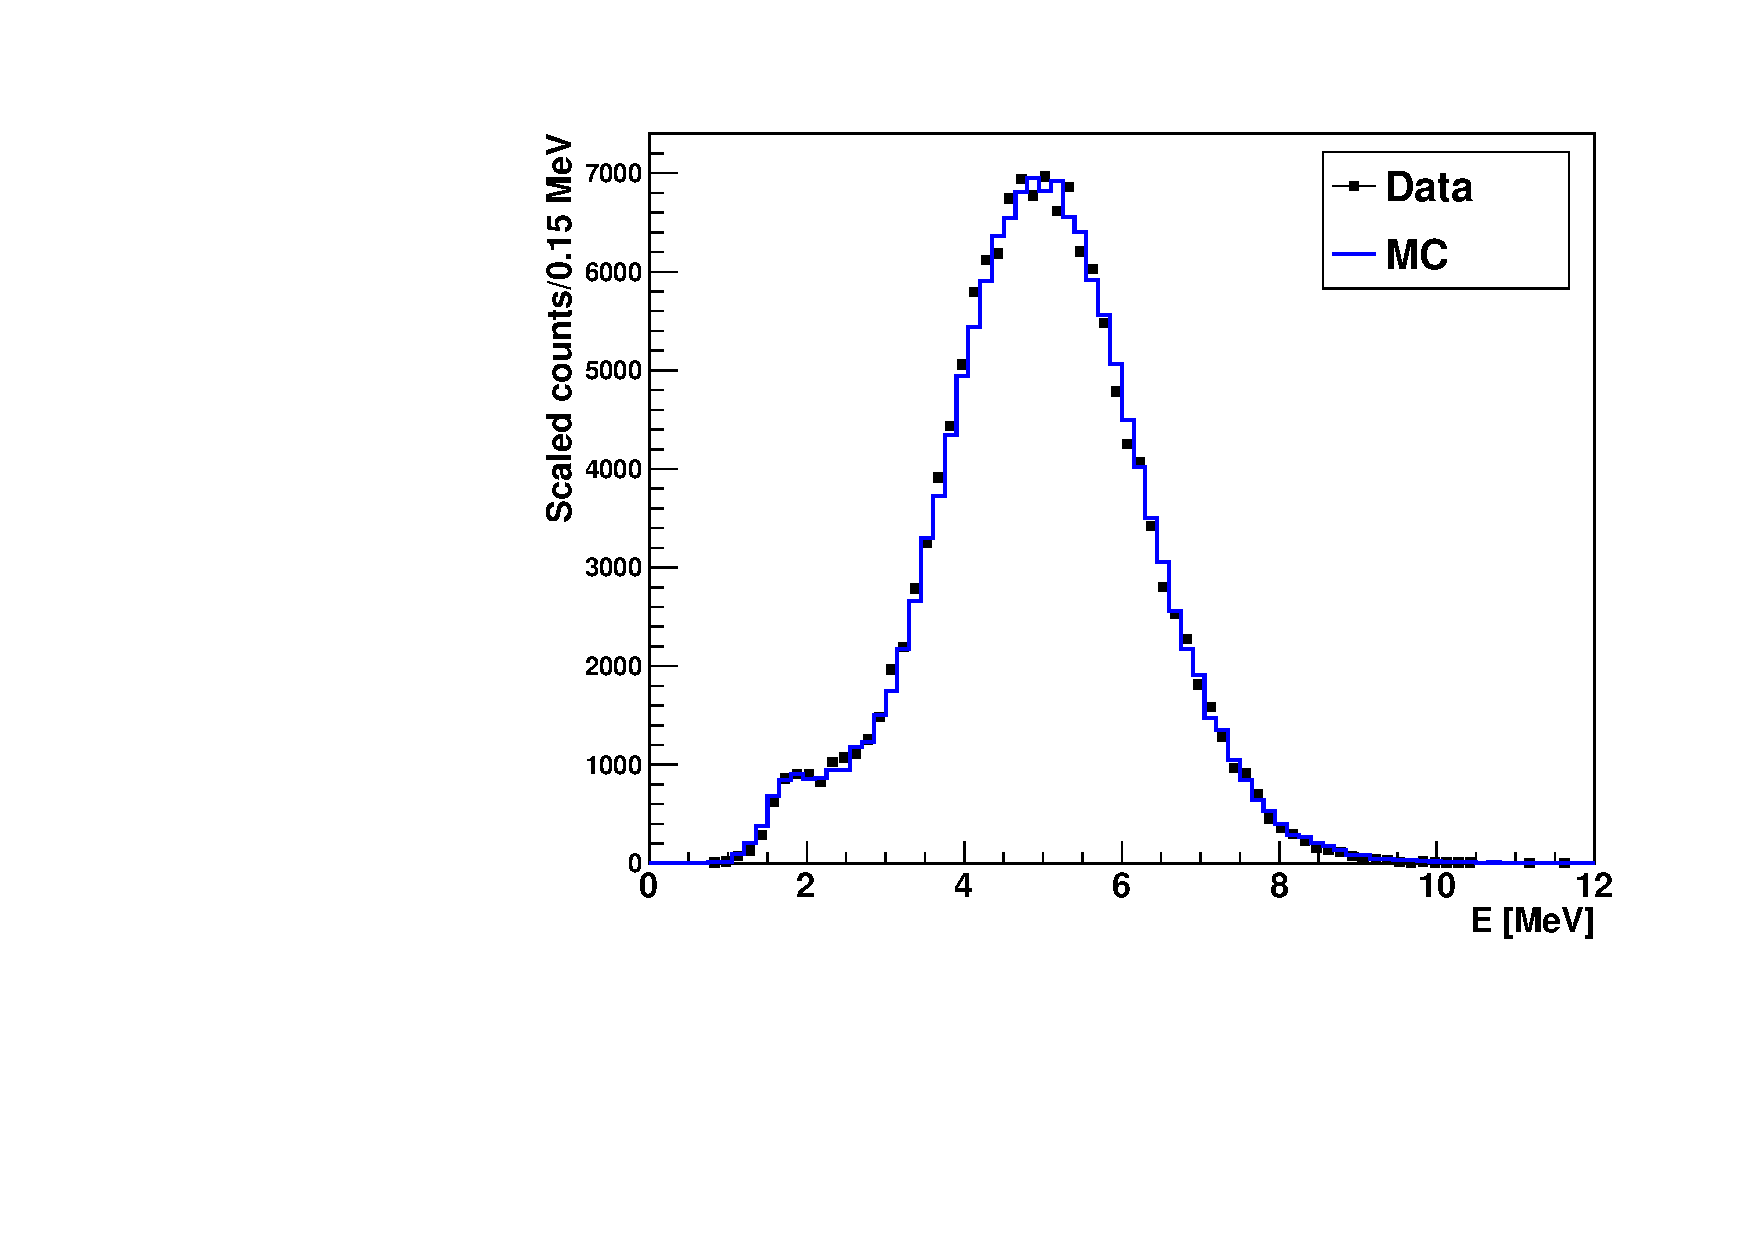
\includegraphics[width=8cm]{N16energyMPWcompare_106925.pdf}}
	\subfigure[$^{16}$N run-107055]{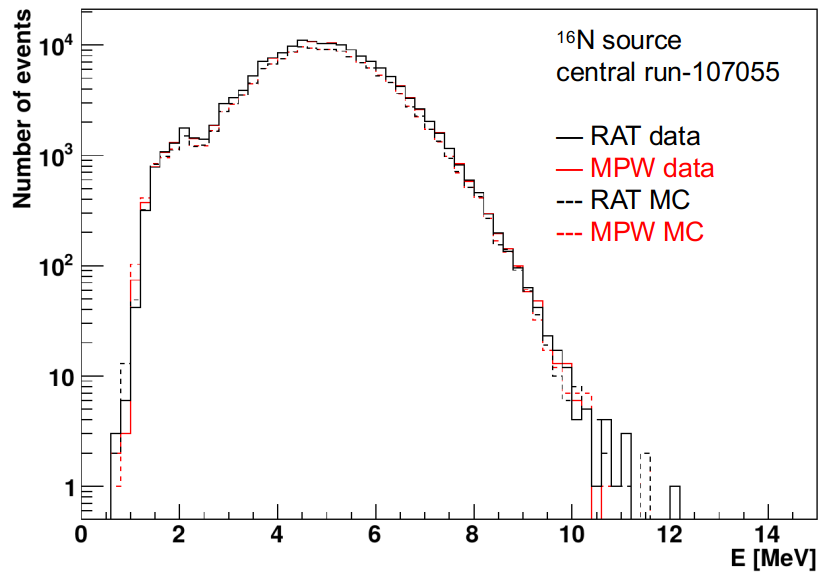
\includegraphics[width=8cm]{N16_reconE_107055.png}}
	\caption[Reconstructed energy spectrum from the $^{16}$N central run-106925 and 107055.]{Reconstructed energy spectrum from the $^{16}$N central run-106925 (top) and 107055 (bottom). For the run-106925 (top), the reconstructed data (black dots) are compared to the MC (blue line), both are \texttt{MPW fitter} results; for the run-107055 (bottom), the \texttt{MPW fitter} results and the \texttt{RAT} results are also compared. Dashed lines for the MC and solid lines for data; red for the \texttt{MPW fitter} results and black for the \texttt{RAT} results.}
	\label{fig:N16energy}	
\end{figure}

\begin{figure}[htbp]
	\centering
	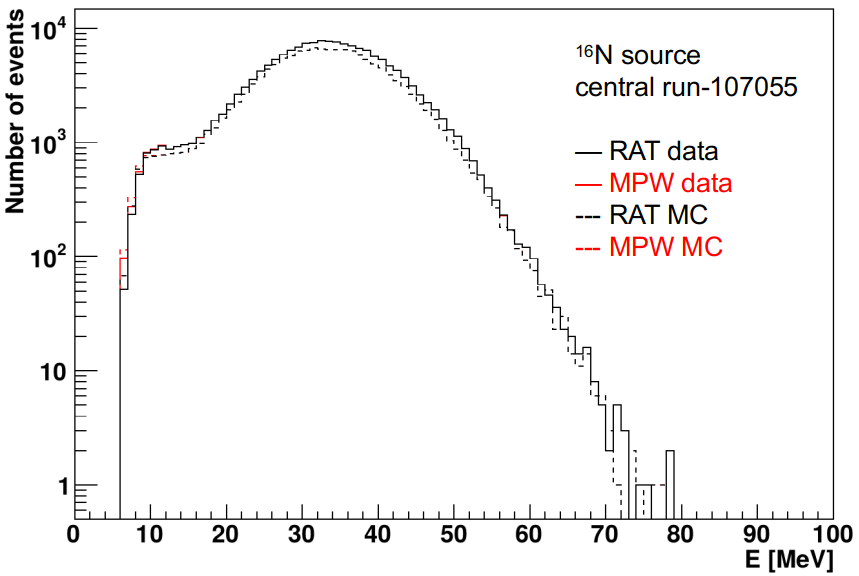
\includegraphics[width=10cm]{N16_nhits_107055.png}
	\caption[NHit spectrum for the $^{16}$N central run-107055.]{NHit spectrum for the $^{16}$N central run-107055. Dashed lines for the MC and solid lines for data; red for the MPW fitter results and black for the \texttt{RAT} results.}
	\label{N16nhits}
\end{figure}

\begin{figure}[htbp]
	\centering
	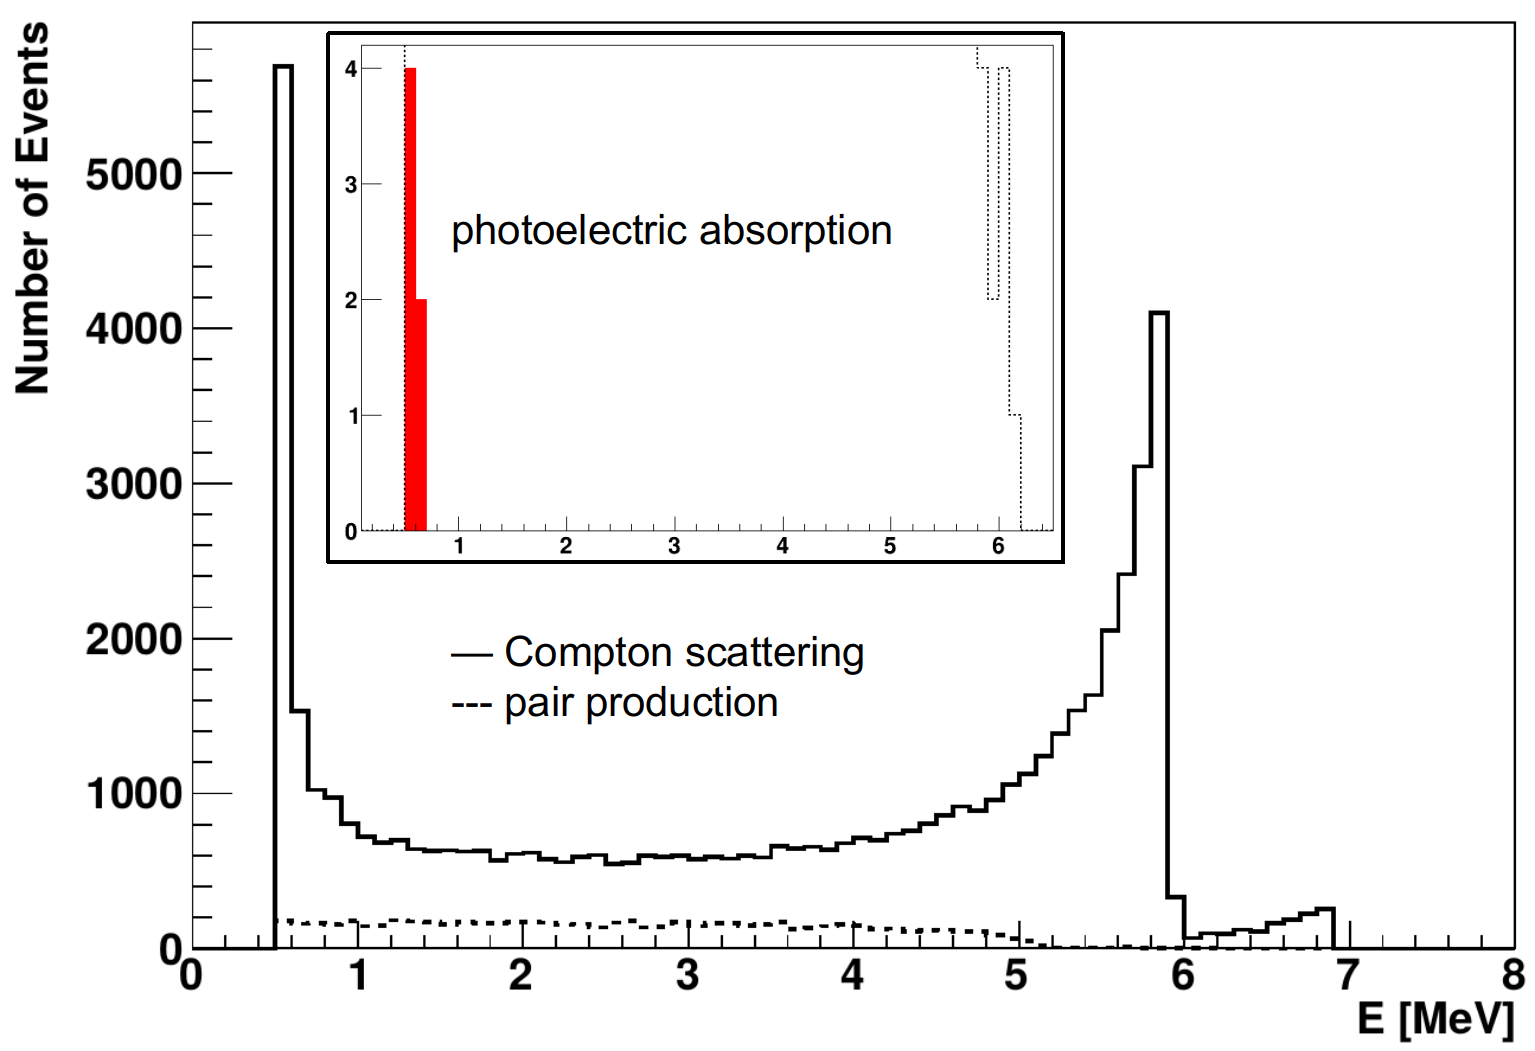
\includegraphics[width=12cm]{N16_MCenergySpectrum.png}
	\caption[Simulated $^{16}$N energy spectrum for different processes.]{Simulated $^{16}$N energy spectrum for different processes, extracted from $10^5$ MC simulations.}
	\label{N16nhitsSimu}
\end{figure}

\begin{figure}[htbp]
	\centering
	\subfigure[MPW data]{ 
		\begin{minipage}[t]{0.4\textwidth}
			\centering
			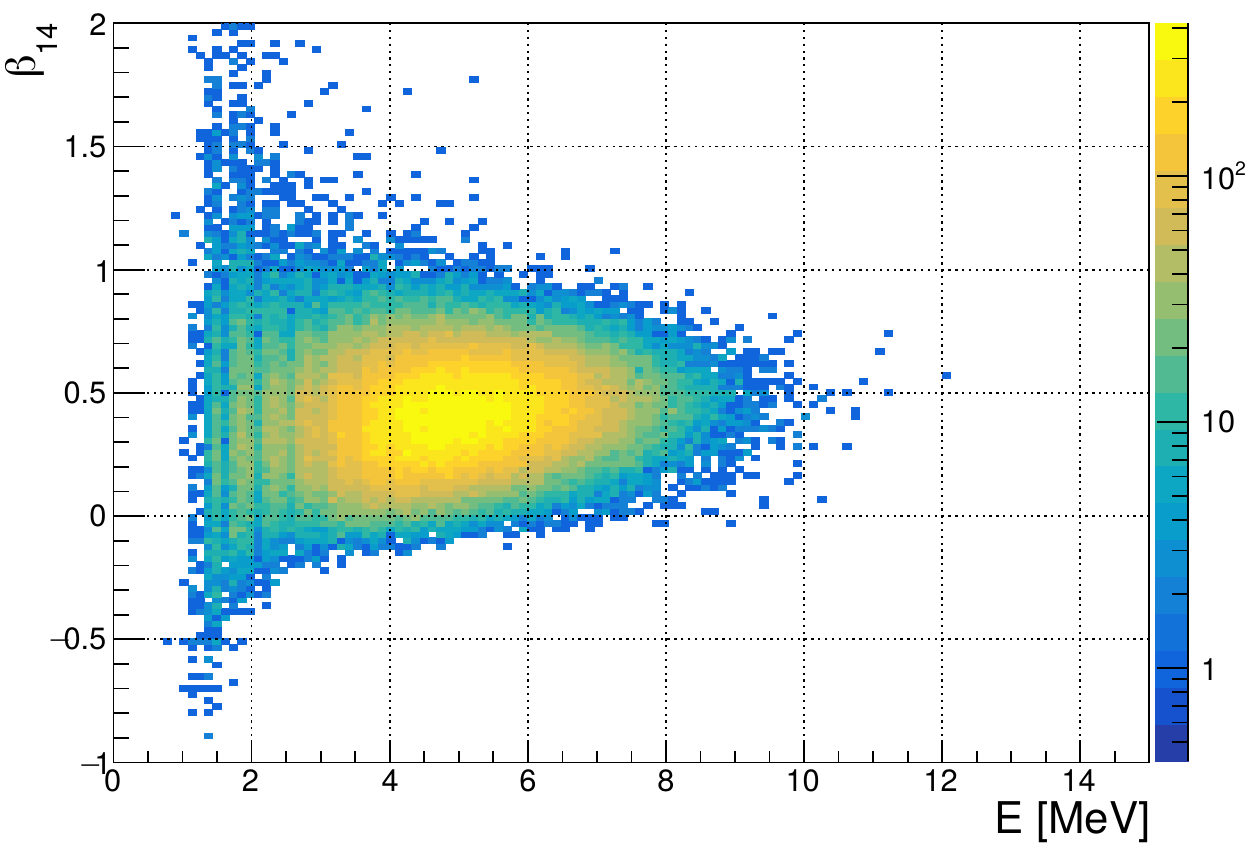
\includegraphics[width=6cm]{N16_MPW_data_EvsBeta14.png}
		\end{minipage}
	}
	\subfigure[MPW MC]{ 
		\begin{minipage}[b]{0.4\textwidth}
			\centering
			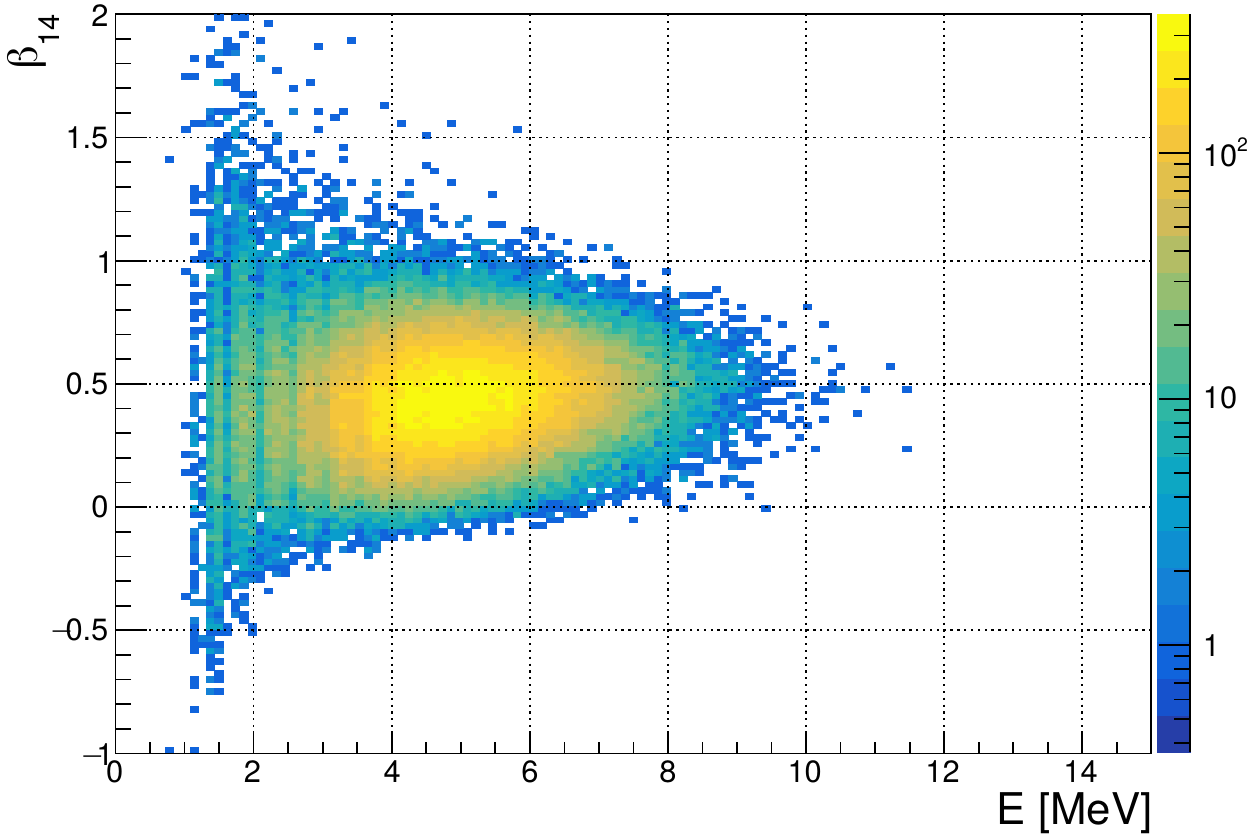
\includegraphics[width=6cm]{N16_MPW_mc_EvsBeta14.png}
		\end{minipage}
	}
	\subfigure[\texttt{RAT} data]{ 
		\begin{minipage}[t]{0.4\textwidth}
			\centering
			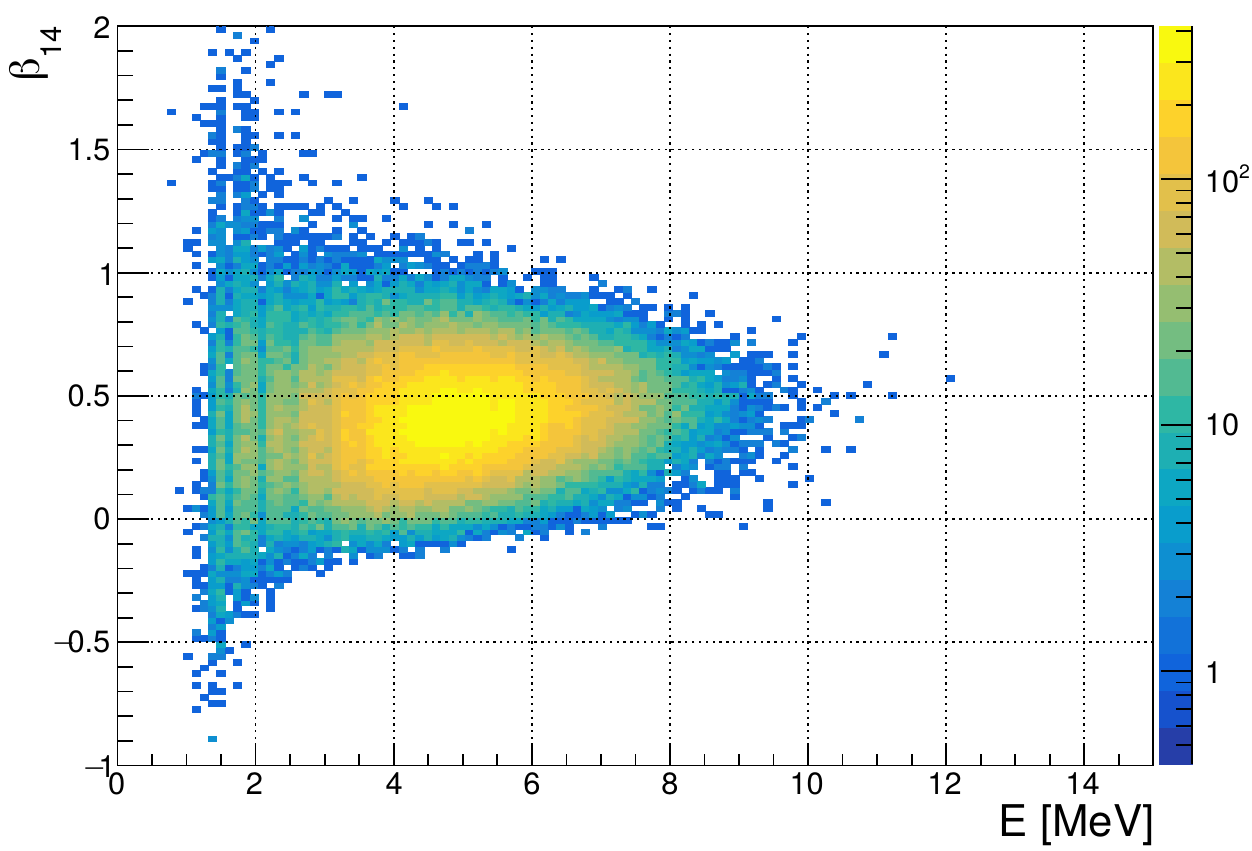
\includegraphics[width=6cm]{N16_rat_data_EvsBeta14.png}
		\end{minipage}
	}
	\subfigure[\texttt{RAT} MC]{ 
		\begin{minipage}[t]{0.4\textwidth}
			\centering
			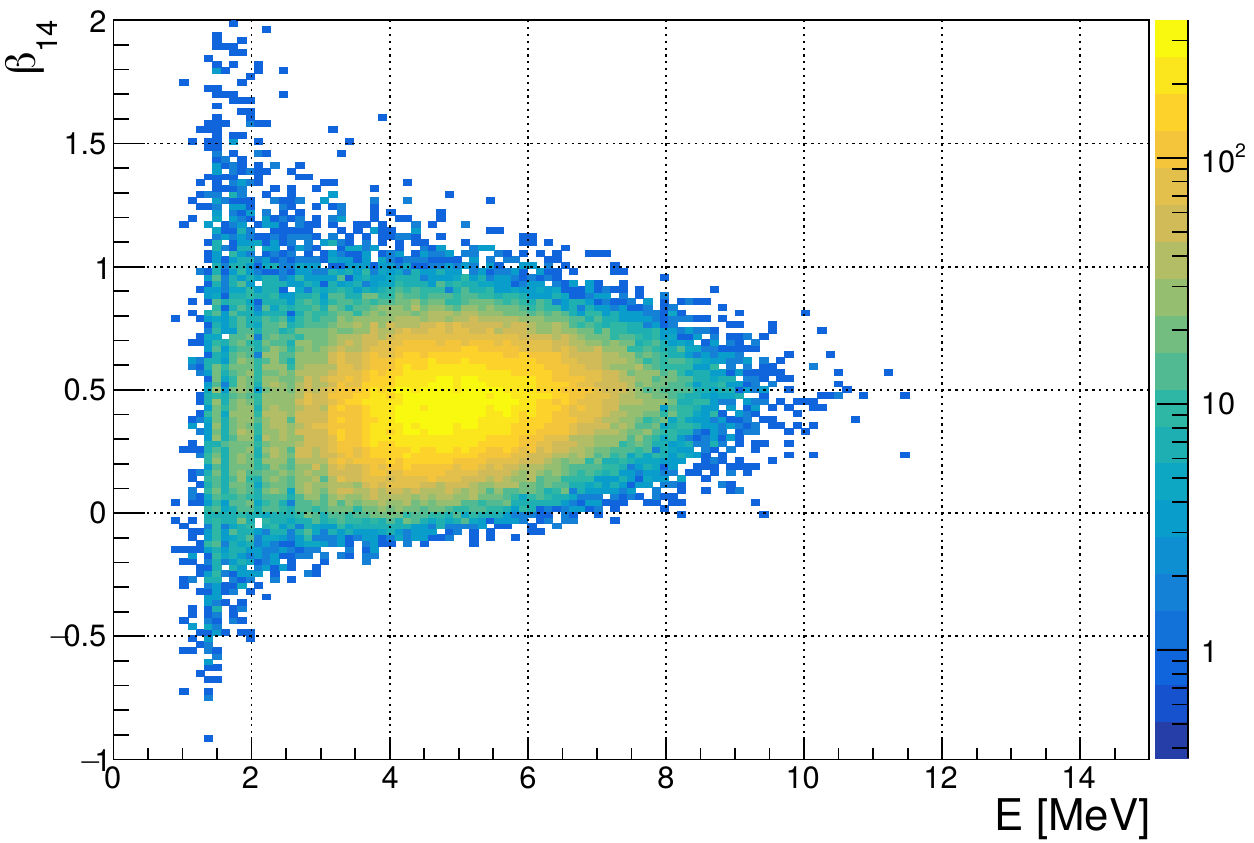
\includegraphics[width=6cm]{N16_rat_mc_EvsBeta14.png}
		\end{minipage}
	}
	\caption[$E_{fit}$ vs $\beta_{14}$ for the data and MC.]{$E_{fit}$ vs $\beta_{14}$ for the data and MC. Both the \texttt{RAT} and the \texttt{MPW} results are shown.}
	\label{EvsBeta14}
\end{figure}

\subsubsection{Energy Resolutions}
Following the methods described in Ref.~\cite{askins2015physics,waterunidoc}, a map that relates the number of Cherenkov photons to the electron energy is created by simulating mono-energetic electrons events with different energies at the detector center, as shown in Fig.~\ref{N16energyMap} (a). By looking up the map and applying linear interpolation, the number of the photons created from the $^{16}$N source is converted into an effective or apparent electron energy spectrum ($P_{source}(T_e)$)\cite{waterunidoc}. Fig.~\ref{N16energyMap} (b) shows the effective electron spectrum of the $^{16}$N central run-107055.

\begin{figure}[htbp]
	\centering
    \subfigure[]{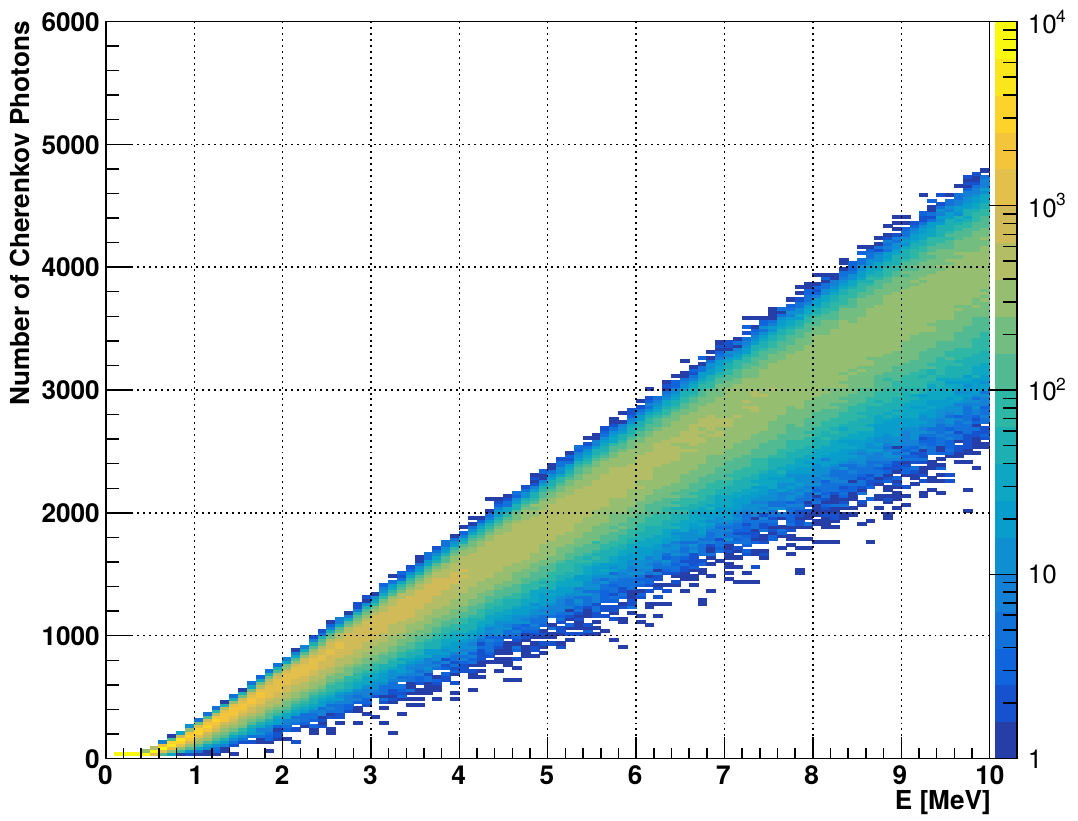
\includegraphics[width=8cm]{2dmap_EvsNphoton.png}}
	\subfigure[]{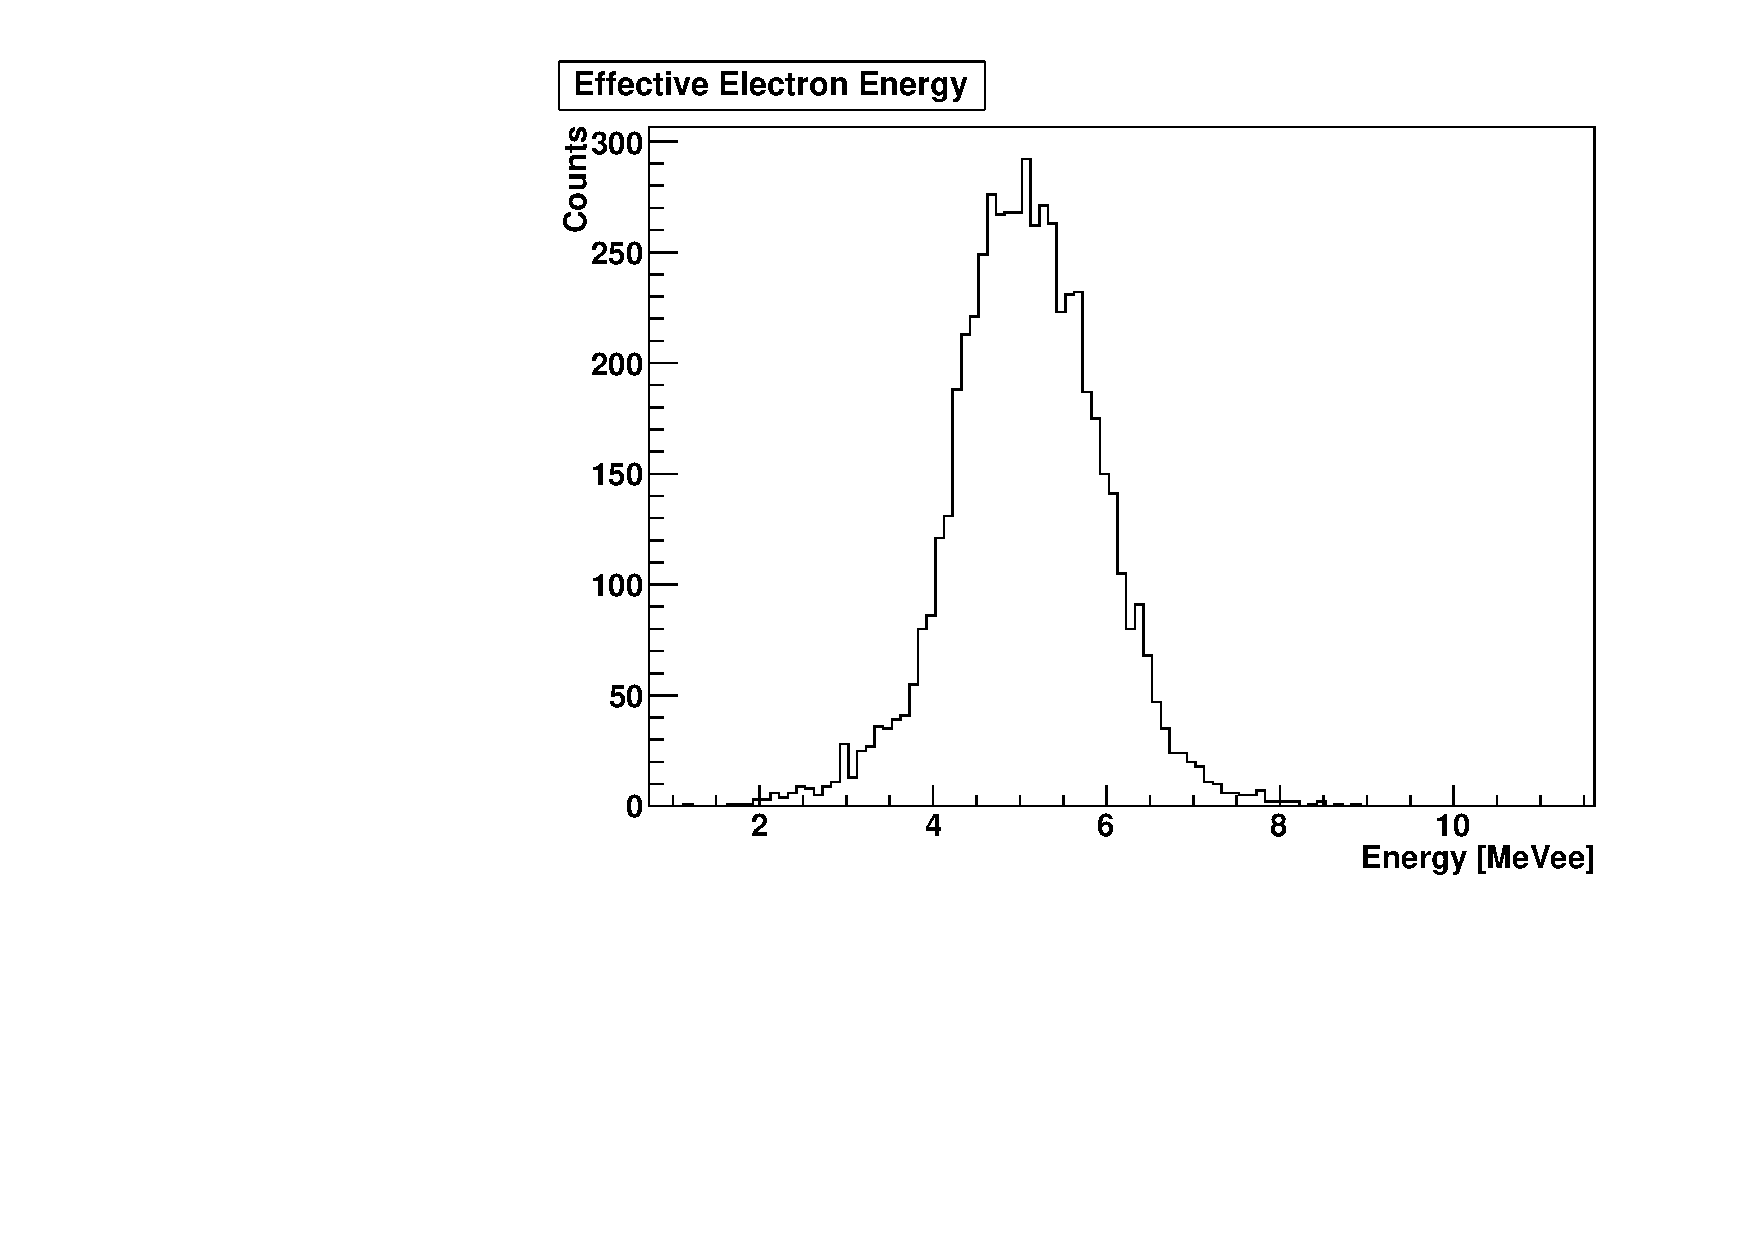
\includegraphics[width=8cm]{N16_run107055_apparentEnergy.pdf}}
	\caption[Converting number of photons to effective electron spectrum.]{Converting number of photons to effective electron spectrum. (a): A 2D map of Electron energy vs number of Cherenkov photons. (b):	Effective electron spectrum of $^{16}$N central run-107055.\label{N16energyMap}}
\end{figure}

To obtain the energy reconstruction resolutions, the reconstructed energy spectrum $P(T_{eff})$ is fitted with the energy resolution function defined as\cite{waterunidoc}:

\begin{equation}
P(T_{eff})=N\int P_{source}(T_e)\frac{1}{\sqrt{2\pi}\sigma_E}\exp \{-\frac{[(1+\delta_E)T_{eff}-T_e]^2}{2\sigma_E^2}\},
\end{equation}
where the predicted apparent energy spectrum, $P_{source}(T_e)$, is convolved with a Gaussian resolution function. In the Gaussian function, $\sigma_E$ is the detector resolution and $\sigma_E = b\sqrt {T_{eff}}$, where $b$ is the energy resolution parameter and $\delta_E$ is the energy scale parameter. The $P_{source}(T_e)$ is the apparent energy spectrum.

Before fitting the reconstructed energy spectrum with the energy resolution function, a few cuts were applied on both the data and MC: the position FoM cut $scaleLogL>10$ and the energy FoM cuts: $0<G_{test}<1.9$, $U_{test}<0.95$ and $-11<Z_{factor}<1$ mentioned in the previous sections were used; the cuts of NHit$>5$, $ITR>0.55$ and $-0.12<\beta_{14}<0.95$ were used to remove instrumental backgrounds; a distance cut: $|\vec{X}_{fit}-\vec{X}_{src}|>700~mm$ was suggested by Refs.~\cite{leta,waterunidoc} to remove the shadow effects when the events are close to the source container; for the event reconstructed within the $700~mm$ distance, if its direction $\vec{u}_{fit}$ is within 45$^\circ$ of the vector from the source to its vertex, i.e., if $\sqrt2/2<\vec{u}_{true}\cdot \vec{u}_{fit}<1$, its energy will also be kept.

A fit range of [3.5, 6.0]~MeV was suggested by Ref.~\cite{waterunidoc} to remove poorly reconstructed events due to the trigger inefficiency. Fig.~\ref{fittedEnergyResol} shows the energy resolution function fitted with the reconstructed energy spectrum of the $^{16}$N central run-107055 data, after applying the cuts mentioned above.
\begin{figure}
	\centering
	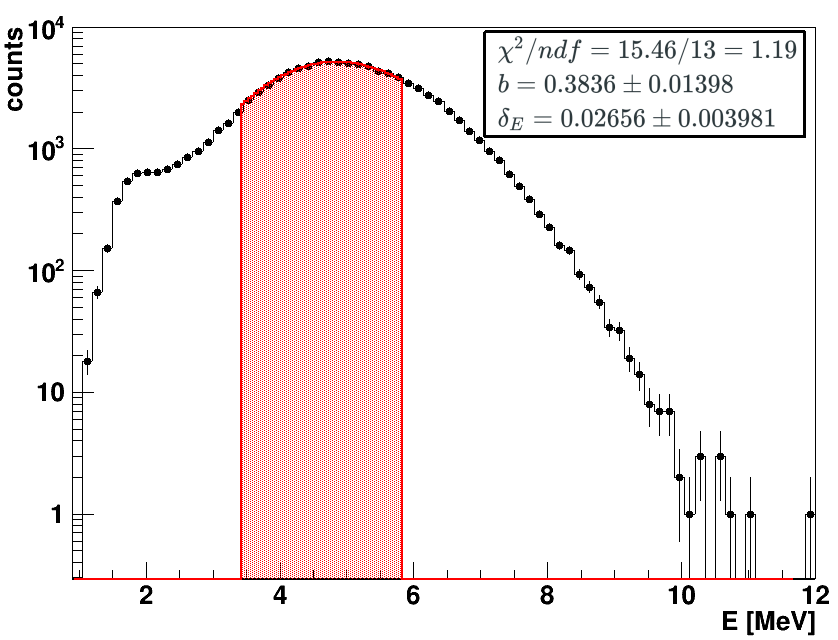
\includegraphics[width=8cm]{N16data_energy_fitted_107055.png}
	\caption[The reconstructed energy spectrum fitted with resolution function.]{The reconstructed energy spectrum of central run-107055 data, fitted with the resolution function (red).}
	\label{fittedEnergyResol}
\end{figure}

For all the internal scans, Fig.~\ref{fig:EscaleVsR} and Fig.~\ref{fig:EresolVsR} show the energy scale ($\delta_E$) and energy resolution ($b$) as a function of the radius of the source manipulation positions. Both the data and MC are shown.
\begin{figure}
	\centering
    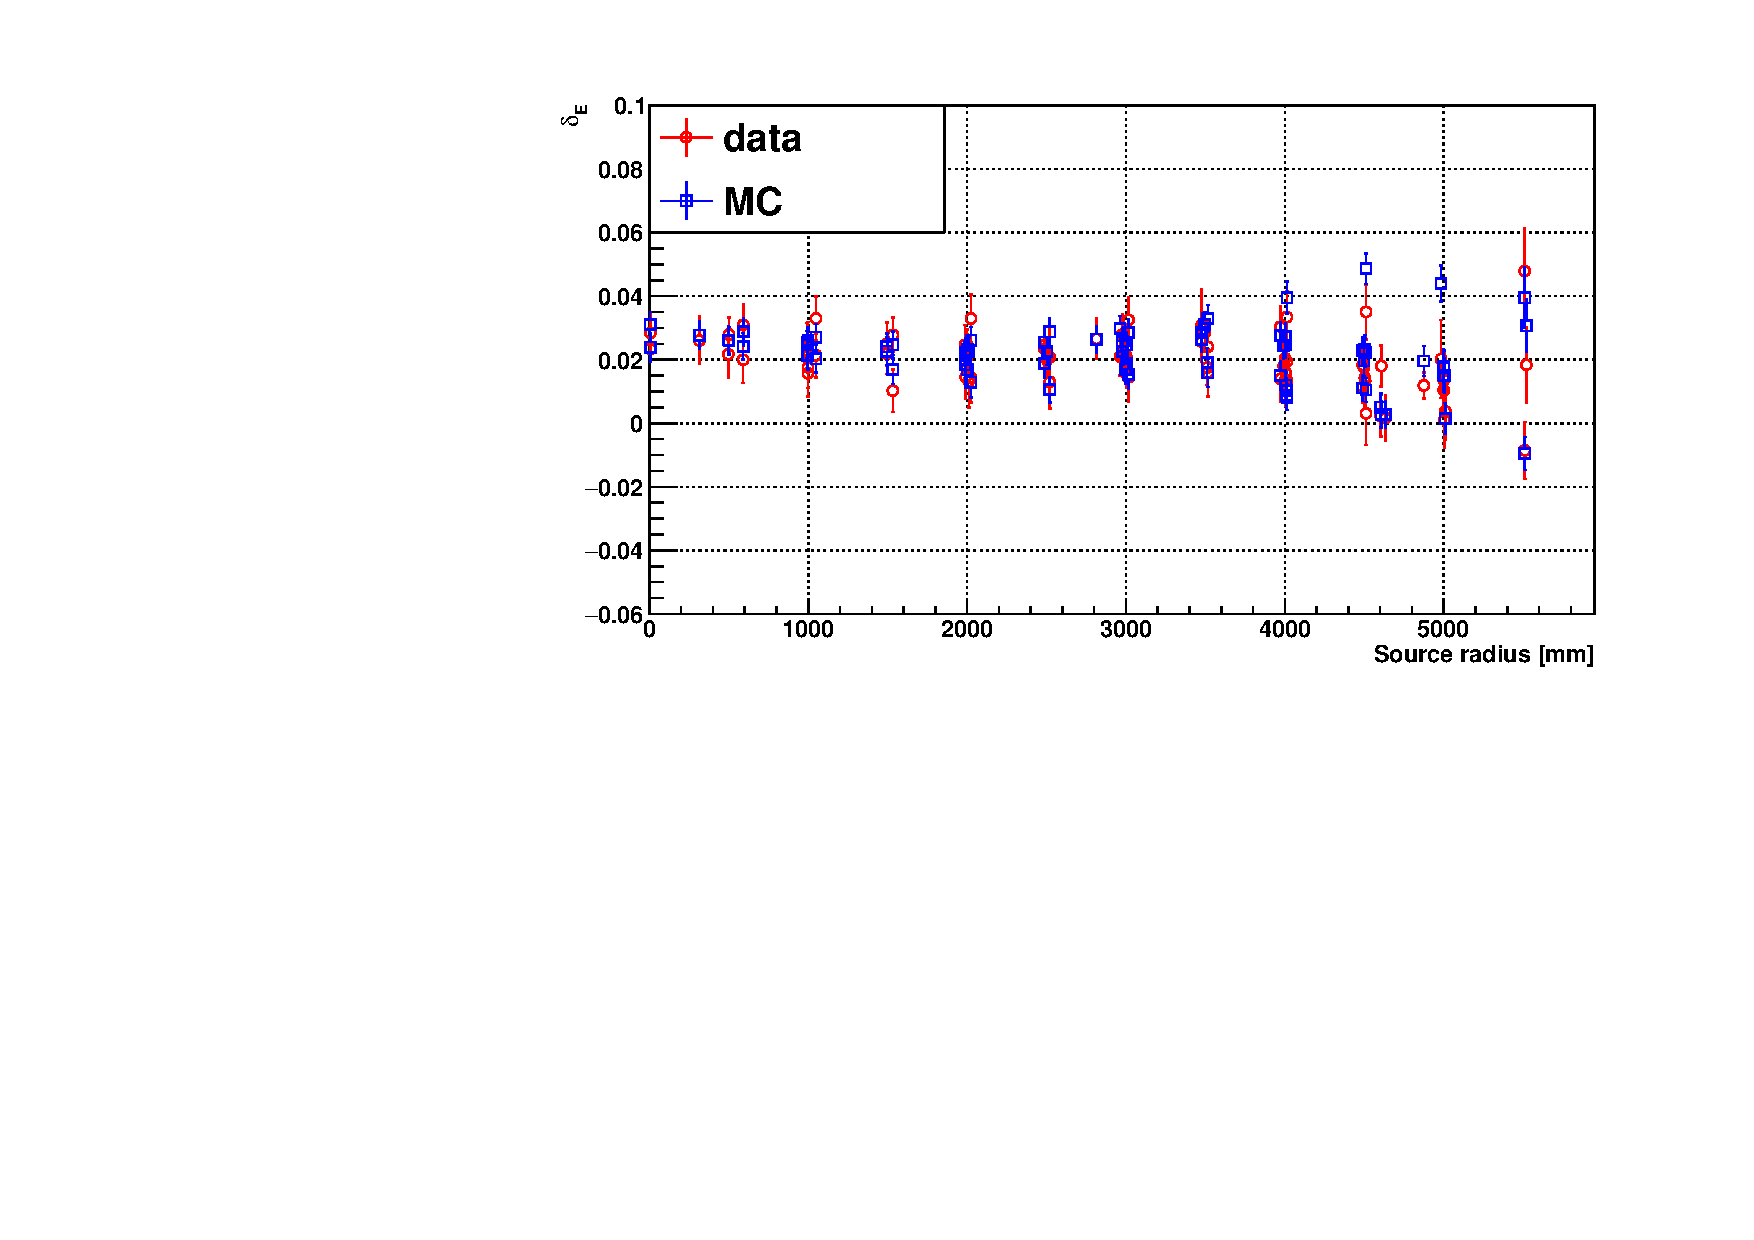
\includegraphics[width=12cm]{EscaleVsSrcRadius.pdf}
	\caption[Fitted energy scales ($\delta_E$) as a function of the source radial manipulation position.]{Fitted energy scales ($\delta_E$) as a function of the source radial manipulation position. Red circles for data and blue squares for the MC.}
	\label{fig:EscaleVsR}
\end{figure}

\begin{figure}
	\centering
	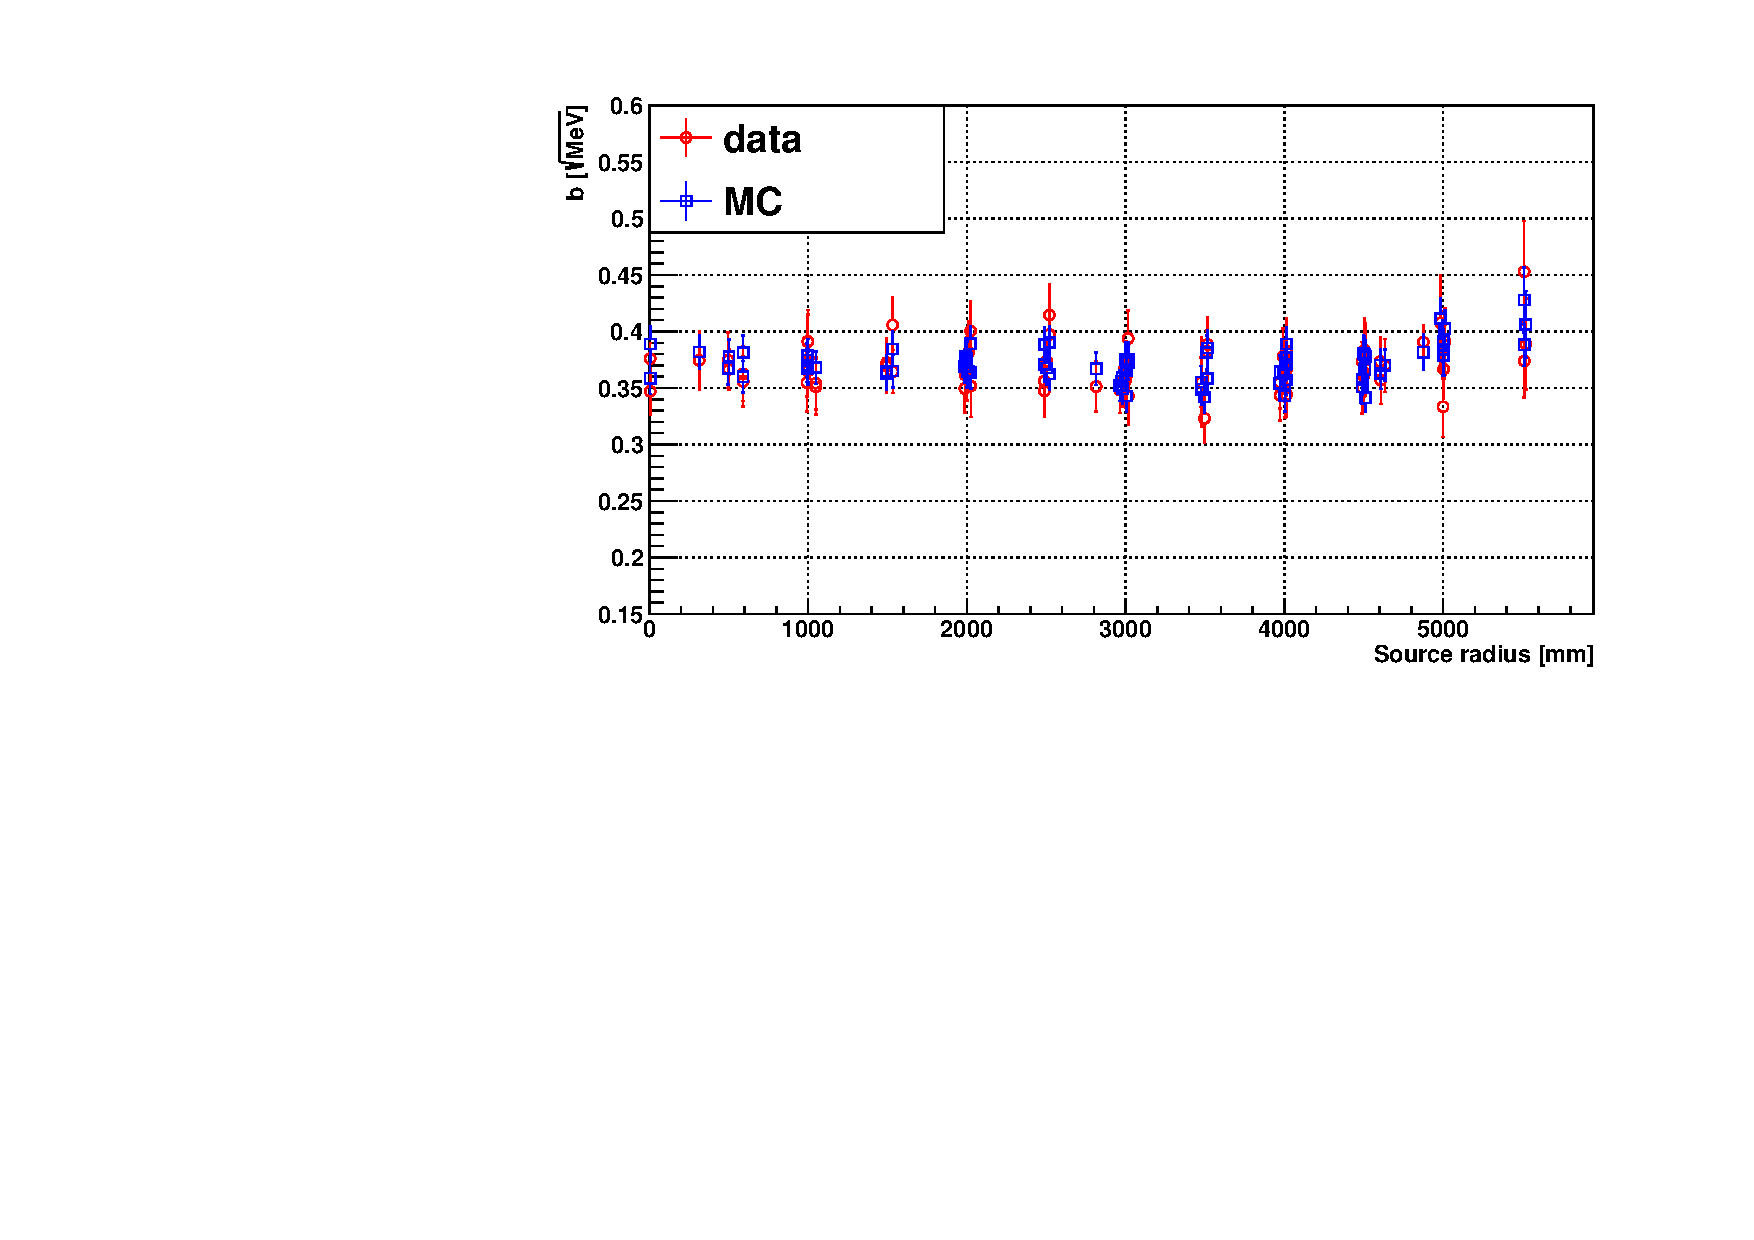
\includegraphics[width=12cm]{EresolVsSrcRadius.pdf}
	\caption[Fitted energy resolutions ($b$) as a function of the source radial manipulation position.]{Fitted energy resolutions ($b$) as a function of the source radial manipulation position. Red circles for data and blue squares for the MC.}
	\label{fig:EresolVsR}
\end{figure}

\subsubsection{Energy Uncertainties}\label{sect:eneryUncertianties}
By comparing the differences between data and MC, the uncertainties of the energy scale $\delta_E$ and resolution $b$ are calculated as:
\begin{equation}
\Delta^2_{\delta}= (\delta_{data}-\delta_{MC})^2+\mathrm{Error}^2_{\delta,data}+\mathrm{Error}^2_{\delta,MC},
\end{equation}
where $\delta=b$ or $\delta_E$, and $\Delta_b=\sqrt{\Delta^2_{b}}$ since the resolution is always positive; while $\Delta_{\delta_E}=\pm\sqrt{\Delta^2_{\delta_E}}$. The fit errors in data and MC were also included in the uncertainties.

Taking the $^{16}$N scan runs within $r<6~m$, the averaged uncertainties are: $\overline{\Delta_{\delta_E}}=0.0107$ and $\overline{\Delta_{b}}=0.0369$. For the $^{16}$N scan runs within $r<5.5~m$, which is the fiducial volume of the solar neutrino analysis mentioned in Chapter 6, $\overline{\Delta_{\delta_E}}=0.0100$ and $\overline{\Delta_{b}}=0.0320$.

To apply the energy scale systematics, the reconstructed energy $E_{fit}$ is smeared by $E'_{fit}=(1\pm\Delta_{\delta_E})\cdot E_{fit}$, where the ``$+$" sign is for scaling up the energy while ``$-$" for scaling down. Fig.~\ref{fig:EscaleSmear} shows the effects of smearing the energy scales on the reconstructed energy spectrum of the $^{16}$N central run-107055. It is obvious that scaling up the $E_{fit}$ widen the $E_{fit}$ spectrum while scaling down the $E_{fit}$ narrows the spectrum. 
\begin{figure}
	\centering
	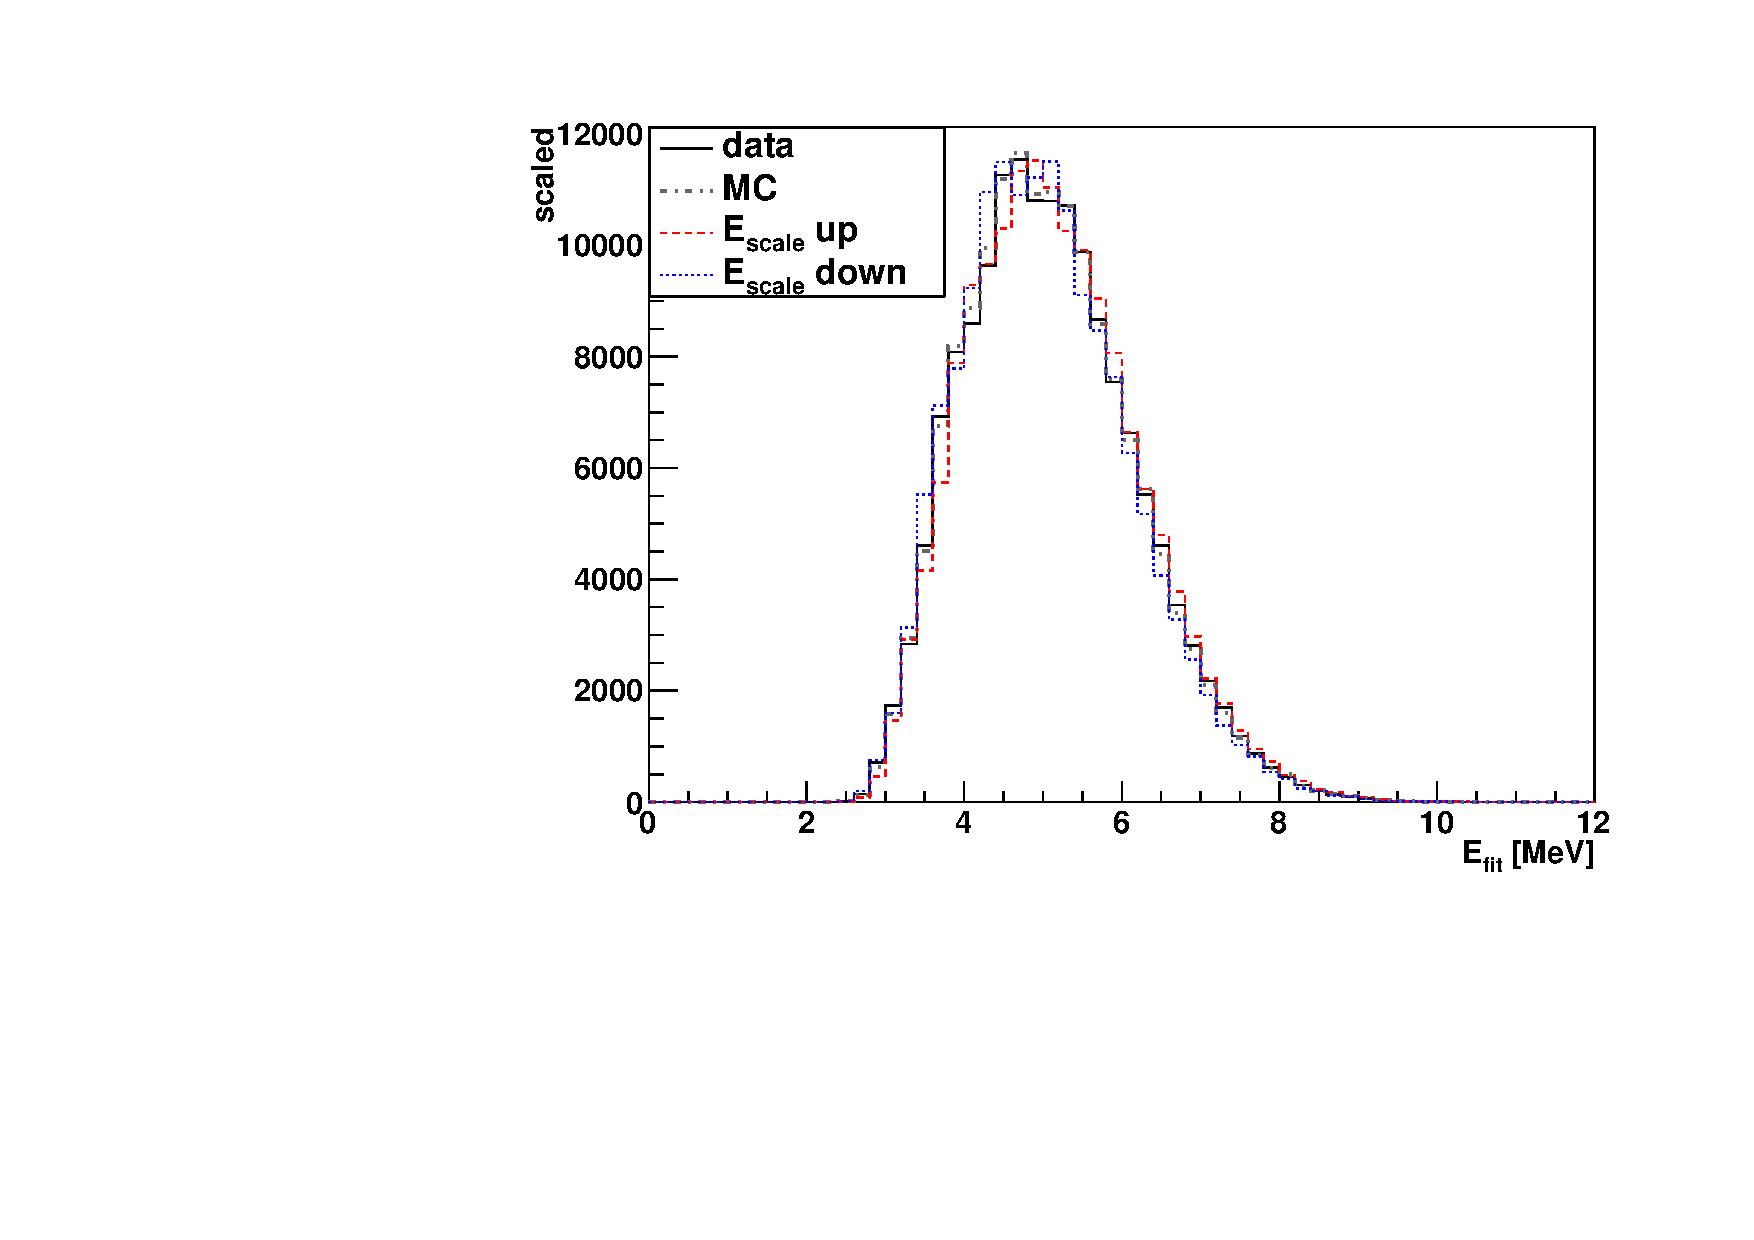
\includegraphics[width=10cm]{SmearedEscale_N16.pdf}
	\caption[Smeared reconstructed energy spectrum of $^{16}$N central run-107055.]{Smeared reconstructed energy spectrum of $^{16}$N central run-107055. The solid black line is for data and the gray dash-dot line is for unsmeared MC; the red dash line is for scaling up the $E_{fit}$ in MC; the blue dot line is for scaling down the $E_{fit}$ in MC. Histograms are normalized to the total counts of the data.}
	\label{fig:EscaleSmear}
\end{figure}

To apply the energy resolution systematics, the spectrum of the reconstructed energy $E_{fit}$ is convolved with an additional Gaussian resolution function $Gaus(0,\sigma_{smear})$, where $\sigma_{smear}=\sqrt{E_{fit}}\cdot\sqrt{(1+\Delta_{b})^2-1}$. To smear the $E_{fit}$ event by event, $E_{smear}$ is randomly sampled from $Gaus(0,\sigma_{smear})$, and then $E'_{fit}=E_{fit}+E_{smear}$. Fig.~\ref{fig:EresolSmear} shows the effects of smearing the energy resolution on the $E_{fit}$ spectrum of the $^{16}$N central run-107055. It is obvious that smearing with the additional resolution coming from the uncertainties in $b$ widen the $E_{fit}$ spectrum. Because there is no unfolding procedure to improve or narrow the energy resolution, this energy resolution systematic is one-sided\cite{marzec2019measurement}. Therefore, in the analysis in Chapter 6, I simply took symmetric uncertainties with different signs.
\begin{figure}
	\centering
	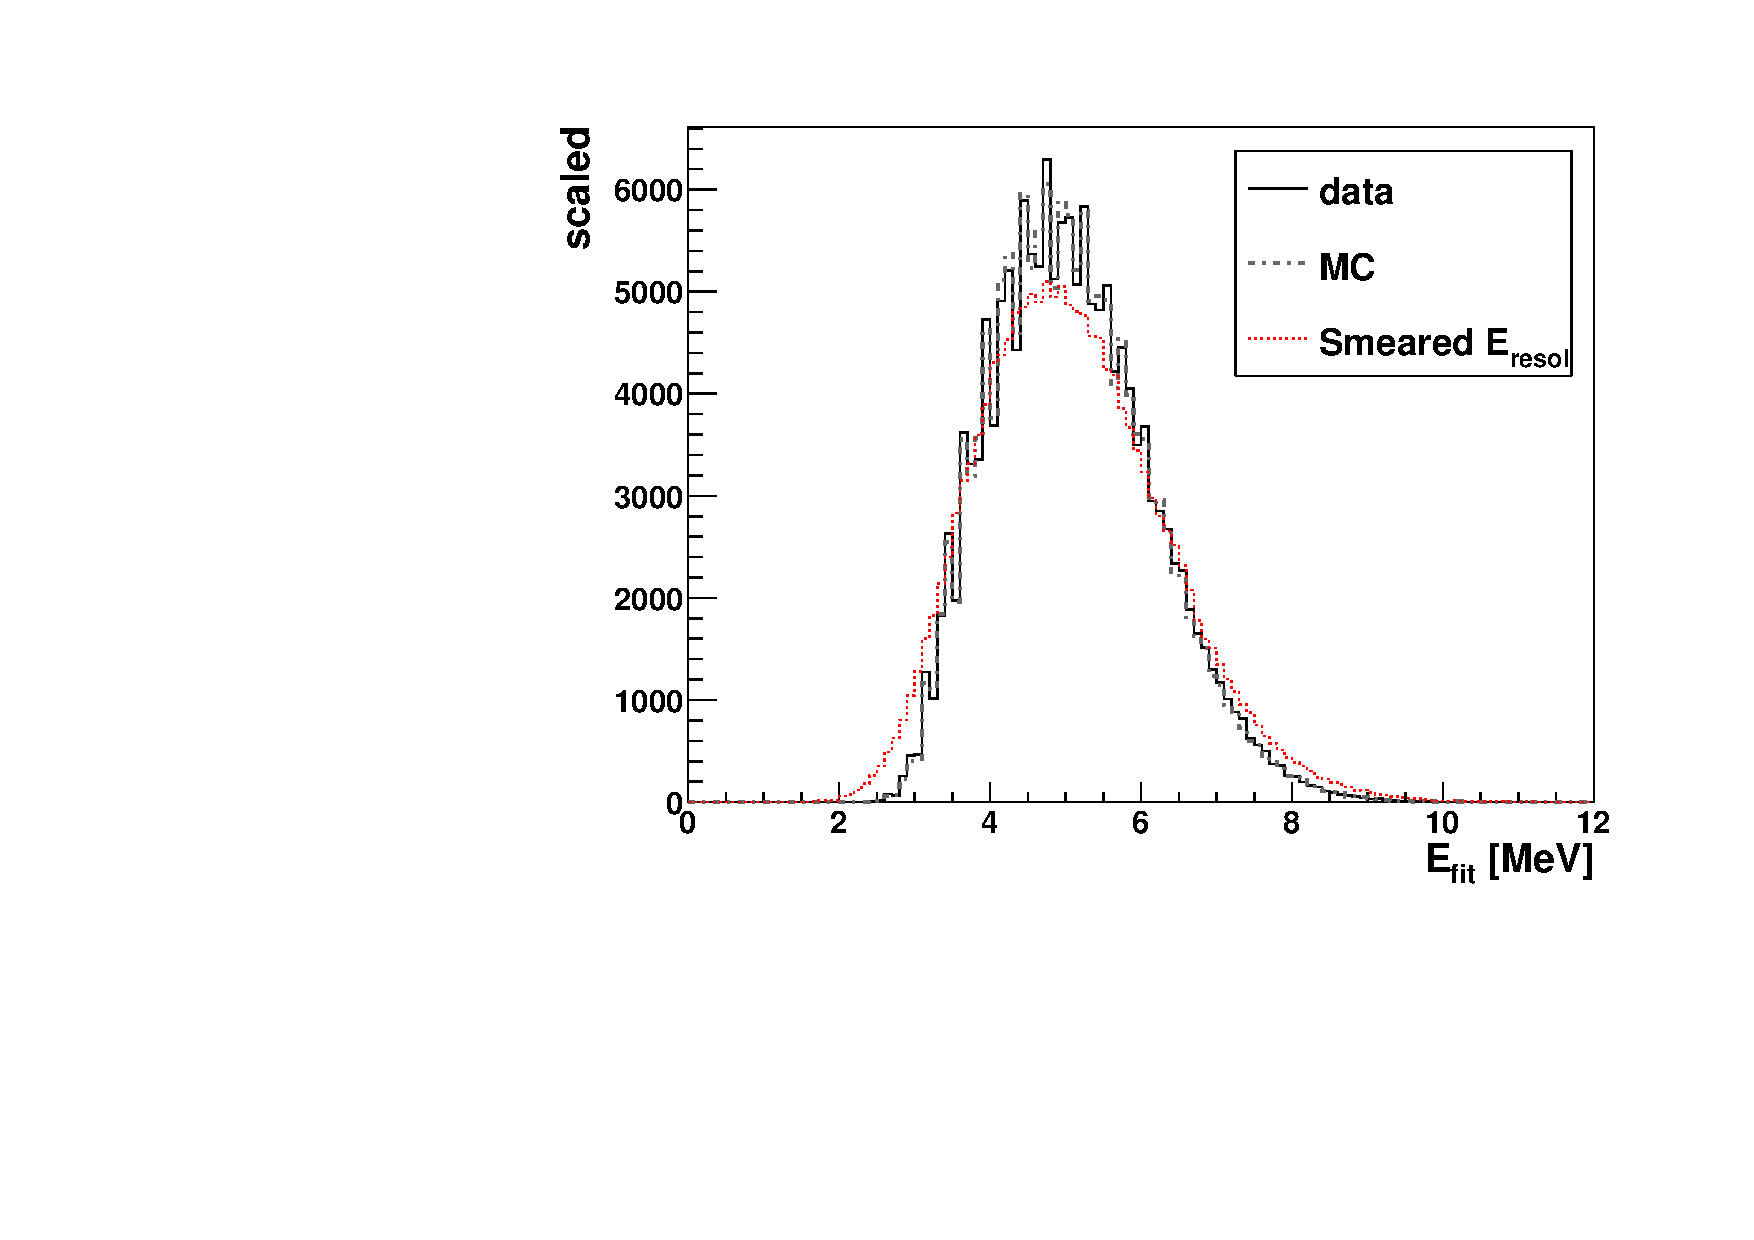
\includegraphics[width=10cm]{SmearedEresol_N16_new.pdf}
	\caption[Smeared reconstructed energy spectrum of $^{16}$N central run-107055.]{Smeared reconstructed energy spectrum of $^{16}$N central run-107055. The red dash line is for smearing the $E_{fit}$ with $Gaus(E_{fit},\sigma)$. Histograms are normalized to the total counts of the data.}
	\label{fig:EresolSmear}
\end{figure}
